\documentclass[14pt]{article}

\usepackage{Packages}
\usepackage{Commands}
\graphicspath{ {C:/Users/Admin/Documents/Github/ProjectMagnet/Расчёты .ipynb/Images/} }

\begin{document}

\begin{titlepage}
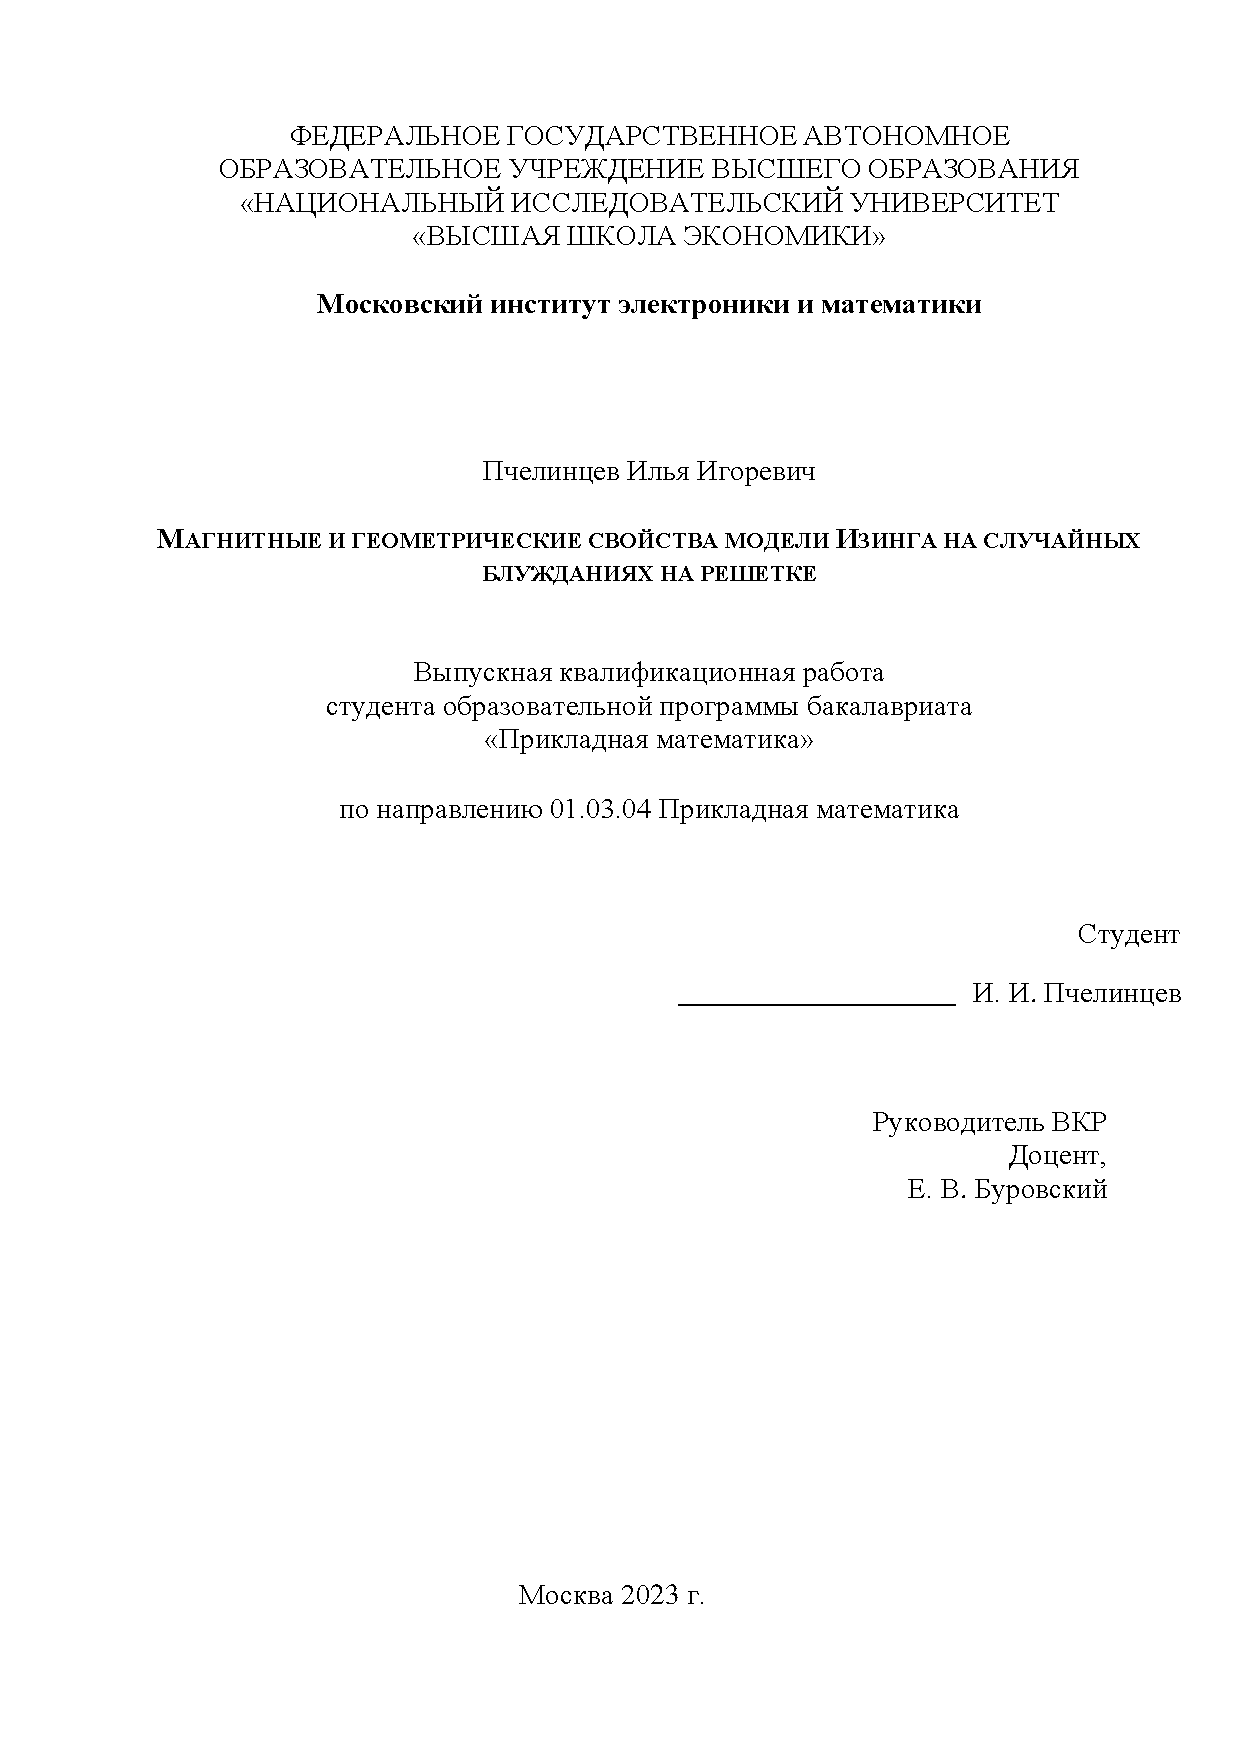
\includepdf[pages={1}]{вкр_титул.pdf}
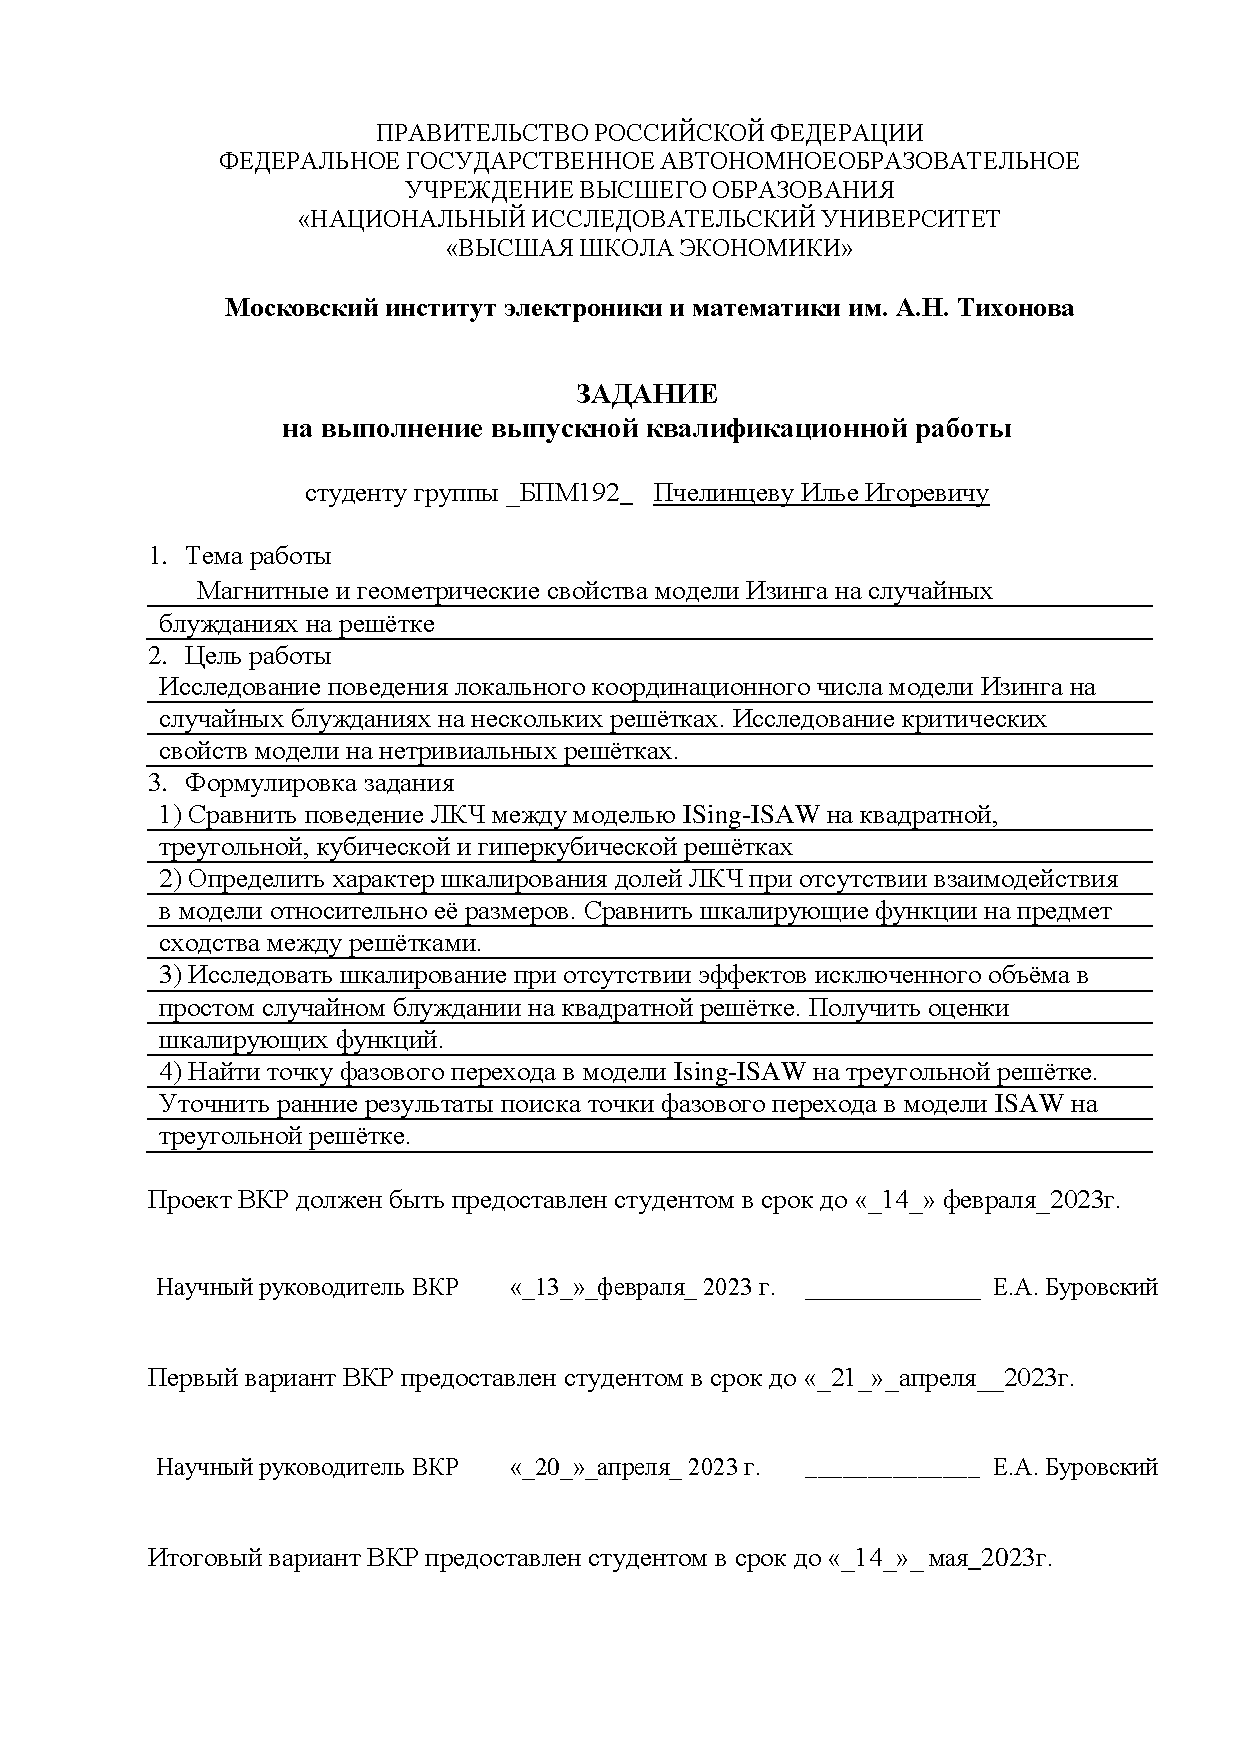
\includepdf[pages={1-2}]{тз_ВКР.pdf}
\end{titlepage}

\begin{abstract}
Данная работа посвящена исследованию магнитного полимера в виде модели случайного блуждания без самопересечений со спиновой подсистемой.
Модель исследуется на нескольких решётках: кубические решётки размерности $d=2,3,4$, а так же треугольная двумерная решётка.
Исследуется задача динамического беспорядка в каноническом амсамбле: спиновая подсистема и конформация моедли имеют соразмерные времена релаксации, а длина цепочки фиксированная.
Доли узлов с фиксированным числом соседей (далее, доли ЛКЧ, локального координационного числа) определяются как мера локальной плотности блуждания.
С помощью методов Монте-Карло на основе алгоритма Червя, данные величины рассматриваются между моделями на решетках с равными размерностями или координационными числами.
Дополнительно исследуется шкалирование долей ЛКЧ в случае отсутствия в блуждании внутреннего взаимодействия, а так же без условия исключенного объёма.
Так же исследуются критические свойства моделей взаимодействующих и магнитных полимеров на треугольной решётке.
Результаты показали различие точек фазового перехода между моделями на треугольной и ранее известной квадратной решёток, однако их критические экспоненты оказались равны.
 \end{abstract}

\renewcommand\abstractname{Abstract}

\begin{abstract}
The study focuses on a model on a magnetic polymer as a chain under excluded volume effects with closely interacting Ising spins.
The model is studied on lattices with different numbers of dimensions $d$: cubic lattice with d=2,3,4 and triangular one with d=2. 
The study focuses on a problem of dynamic disorder in a canonical ensemble, as the model has comparable relaxation times between spin subsystem and conformation, and the fixed length of a chain.
The mean fraction of monomers on a chain with fixed number of neighbors (or bulks) is considered as a geometric measure of the local compaction of conformation.
Using Monte-Carlo methods in Worm-Algorithm, these measures are compared between chains with respective spin-to-spin coupling constant J in lattices having equal coordination number or dimensionality. 
The fractions of the LCN (local coordination number) are also researched by finite-size scaling methods in cases of zero-interaction and disabled excluded volume effects. 
The critical properties of the model were also researched on a triangular lattice.
Our results suggests that the "triangular" theta-point differs from the results for the square lattice, but models on both lattices are appeared to have equal critical expopents.
\end{abstract}
\newpage

\tableofcontents

%\if 0
\section{Введение}

Модель случайных блужданий без самопересечений (далее - СБС) - одна из наиболее широко изученных моделей из класса линейных полимеров. 
Более того, она является одной из простейших моделей для изучения критического поведения - так, в случае когда модель усложнена наличием взаимодействия между ближайшими узлами цепочки, её фазовый переход оказывается зафиксирован между состояниями её растворителя, и при термическом равновесии системы полученная полимерная цепочка будет схлопнутой в условиях сильного растворителя или вытянутой в слабом растворителе.
Трикритичность данного перехода была описана в работе \cite{Gennes1979}.

Влияние близких связей было широко рассмотрено среди класса моделей магнитного полимера, взаимодействие между узлами которых стало ещё более сложным:
каждый узел обладает спином, а сила взаимодействия между ближайшими узлами стала отдельным параметром. 
Её название - модель Изинга на случайном блуждании без самопересечений.
В работе \cite{Garel1999} был рассмотрен случай, когда она так же обладает переменным внешним полем, и все заключения о её магнитных свойствах были оценены в сравнении с моделью среднего поля.
В то же время влияние геометрических свойств модели на магнитные не до конца ясно и их изучение в некоторых случаях требует статистического подхода.

В предыдущей работе \cite{faizullina2021critical} было определено, что фазовый переход двумерной модели Изинга на CБС
имеет непрерывный характер. 
В этой работе мы продолжаем изучать геометрические свойства данной модели и сравнивать их с её родительскими моделями или модификациями, такими как классическая модель Изинга на регулярной решётке, опредёленная в работе \cite{selke2006critical}, и взаимодействующее случайное блуждание без самопересечений в соответствующих критических областях. 
Мы предполагаем, что модели с похожими геометрическими свойствами будут так же иметь схожесть в магнитных, что мы рассмотрим при сравнении кумулянтов биндера в области $\theta$-перехода моделей при равных значениях асферичности.
Также могут быть интересны для рассмотрения решётки, на которых исследуются конформации модели, как параметр задающий закон, по которому определяется близость узлов и следовательно - существование тех или иных связей между ними в цепочке. 
Данное направление было начато в частном случае среди концов случайных блужданий без самопересечений на квадратной решётке в работе \cite{owczarek2008scaling}. 
В нашей работе мы рассмотрим эти результаты с долей узлов с фиксированным количество соседей на квадратной решётке, как обобщение на внутренние узлы цепочки, а так же рассмотрим поведение данного геометрического свойства среди разных решёток в пределе бесконечной длины цепочки.  

\section{Модели и методы}
В рамках данной работы определяется несколько моделей: первой будет модель Изинга на случайном блужданий без самопересечений (далее - Ising-ISAW). Энергия системы конформации $u$ (последовательности точек на решётке, на которых размещёна цепочка) фиксированной длины N с последовательностью спинов в узлах s, принимающих значение $+1$ или $-1$, рассчитывается как сумма взаимодействий между ближайшими узлами цепочки:

\begin{equation}
E(s,u) = -J \sum_{\la i, j \ra} s_i s_j,\ \ \ \ i,j \in u, |u|=N
\end{equation}
Статическая сумма модели берётся по всем возможным последовательностяv ${s}$ и конформациям $u$:

\begin{equation}
Z = \sum_s \sum_u \exp{(\frac{-E}{kT})}
\end{equation}

где $T$ — температура, $k$ — постоянная Больцмана. Без потери общности можно считать $kT = 1$, тем самым оставляя J самостоятелньым параметром модели.
В первой части работы модель Ising-ISAW рассматривается только на квадратной решётке, где соседями узла можно считать мономеры, расположенные сверху, снизу, слева и справа от него.

Под "родительскими" к Ising-ISAW моделями определим следующие две: с одной стороны, взаимодействующая составляющая модели берётся из классических моделей Изинга - в частности, мы будем рассматривать классическую модель Изинга на регулярной прямоугольной решётке (далее - прямоугольный Изинг), определеную так же в работе \cite{selke2006critical}.
В ней узлы со спинами заполняют всю решётку со стороной $L=N_x$ и отношением сторон $r=\frac{N_y}{N_x}$. Длина стороны считается как количество узлов решётки в одном ряде. 
Решётка может иметь как периодический граничные условия - когда узлы на противоположных краях решётки считаются соседними - так 
Тогда энергия системы с последовательностью спинов $s$, рассчитывается как сумма взаимодействий между ближайшими узлами по всей решётке:

\begin{equation}
E(L, r, \{s\}) = -J \sum_{\la i, j \ra} s_i s_j,\ \ \ \ i,j = (x_i, u_i), (x_j, y_j) \in [1..L] \times [1..L*r]
\end{equation}

Статическая сумма модели берётся только возможным последовательностяv ${s}$:

\begin{equation}
Z = \sum_s \exp{(\frac{-E}{kT})}
\end{equation}

В качестве сравниваемого между моделями магнитного свойства определим кумулянт Биндера (или критический кумулянт):

\begin{equation}
\label{eq:Cumulant}
U_{4} = 1 - \frac{\la m^{4} \ra}{3 (m^{2})^{2}}
\end{equation}

где $\la m^{2} \ra$  - средний квадрат удельной намагниченности, $\la m^{4} \ra$ - средная удельная намагниченность в четвертой степени. 

С другой стороны, определелим модель взаимодействующего блуждания без самопересечений (далее - ISAW) на квадратной решётке из работы \cite{caracciolo2011geometrical}.
В отличие от Ising-ISAW, узлы конформации не имеют спинов, и энергия модели рассчитывается как сумма связей переменной силы J между узлами:

\begin{equation}
E(\{u\}) = \sum_{\la i, j \ra} 1,\ \ \ i,j \in u, |u|=N
\end{equation}

\begin{equation}
Z = \sum_s \exp{(- \beta E(\{s\}))}
\end{equation}

В рамках работы \cite{caracciolo2011geometrical} исследовалось поведение геометрических свойств в критической области - в частности, асферичности конформации, показателя отличия системы узлов от круга.
Для этого определим показатели формы системы, такие как тензор вращения системы - матрица корреляции координат системы из N точек $w_i = (w_{i,\alpha}, w_{i,\beta})$:

\begin{equation}\label{eq:Ten_G1}
    Q_{N,\alpha\beta} = \frac{1}{N+1} \sum^{N}_{i=0}(w_{i,\alpha} - w_{c, \alpha})(w_{i,\beta} - w_{c, \beta})
\end{equation}

где $w_{c,\alpha} - \alpha$ -я координата вектора центра масс. В случае, если начало координат расположено в центре масс (следовательно, сумма векторов точек блуждания = 0), формула $\alpha\beta-$элемента тензора упрощается и численно равна второму моменту координаты (если $\alpha = \beta$), или до среднего произведения разных координат по всем точкам блуждания.

\begin{align}\label{eq:Ten_G_C}
    Q_{N,\alpha\beta} = &\frac{1}{(N+1)} \sum_{i=0}^{N} w_{i, \alpha} w_{i, \beta} \\
    \sum^{N}_{i=0}w_{i} &= 0
\end{align}

Собственные значения $q_1, q_2$ полученного тензора вращения можно интерпретировать как квадраты длин полуосей эллипса вращения системы.
Их отношение для системы длины $N$ равна:

\begin{equation}
r = \sqrt{\frac{\la q_1 \ra_N}{\la q_2 \ra_N}}
\end{equation}

Так же эти значения используются для расчёта ещё одного показателя формы -
средней асферичности:

\begin{equation}
\label{eq:Asphericity}
    \mathcal{A} = \left\langle \frac{(q_{1} - q_{2})^{2}}{(q_{1} + q_{2})^{2}} \right\rangle_{N}
\end{equation}

Модификации исследуемой системы Ising-ISAW имеют изменения в выбранной решётке - то есть, законов, по кото
: в работе





\section{Модели и методы}

В рамках данной работы определяется несколько моделей: 
в первую очередь определяется модель взаимодействующего блуждания без самопересечений ISAW. 
Энергия системы ISAW c конформацией $u$ (последовательности узлов решётки, на которых размещёна цепочка) 
фиксированной длины $N$ равна числу связей между ближайшими мономерами в цепочке \eqref{eq:ISAW_ham}:

\begin{equation}
\begin{array}{l}
\label{eq:ISAW_ham}
E(u) = J \sum_{\la i, j \ra} 1\ \ \ \ i,j \in u, |u|=N \\
Z = \sum_u \exp{(\frac{-E}{kT})}
\end{array}
\end{equation}

Модель рассматривается в каноническом амсамбле, поэтому статистическая сумма модели суммирует все возможные конформации $u$ длины $N$.

Так же определим модель Изинга на случайном блужданий без самопересечений (далее - Ising-ISAW).
В мономерах конформации длины $N$ встроена спиновая подсистема $\{s\}$, 
принимающая значение в узлах цепочки $+1$ или $-1$, вследствие чего энергия рассчитывается между ближайшими узлами цепочки как:

\begin{equation}
\label{eq:IsISAW_ham}
E(s,u) = J \sum_{\la i, j \ra} s_i s_j,\ \ \ \ i,j \in u, |u|=N
\end{equation}

Статическая сумма модели берётся по всем возможным последовательностям $\{s\}$ и конформациям $u$ фиксированной длины:

\begin{equation}
Z = \sum_s \sum_u \exp{(\frac{-E}{kT})}
\end{equation}

в обоих представленных моделях $T$ — температура, $k$ — постоянная Больцмана. 
Без потери общности можно считать $kT = 1$, тем самым оставляя J единственным самостоятелньым параметром модели.

Множество $\la i, j \ra$ под знаком суммирования обозначает пары узлов решётки, принадлежащие конформации модели $u$, между которыми лежит ребро исследуемой решётки.
В зависимости от выбранной решётки, для узла конформации меняется множество узлов решётки, 
которые могут считаться "ближайшими" к нему, ровно как и максимальное количество связей у одного мономера - так называемое "координационное число" решётки.
Так, квадратной решётке (левый рисунок \ref{fig:lattices}) соседями узла можно считать мономеры, расположенные сверху, снизу, слева и справа и него, 
в то время как в треугольной решётке соседними так же считаются и узлы на одной из диагоналей, проходящей через узел решётки,
а на кубической – к соседним приравнены узлы с теми же координатами на соседних плоскостях решётки.
Узел 4D-гиперкубической решётки имеет 8 соседей, каждый из которых отличается в одной координате на ±1 от рассматриваемого узла.

\begin{figure}
    \centering
    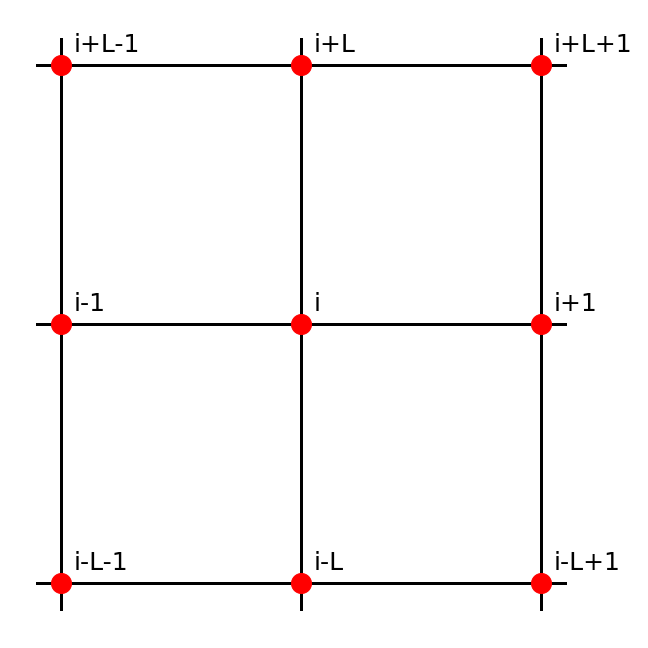
\includegraphics[width=0.3\textwidth]{SqLattice2.png}\ \ \ \ \ \ \ \ \ \ \ \ \ \ 
    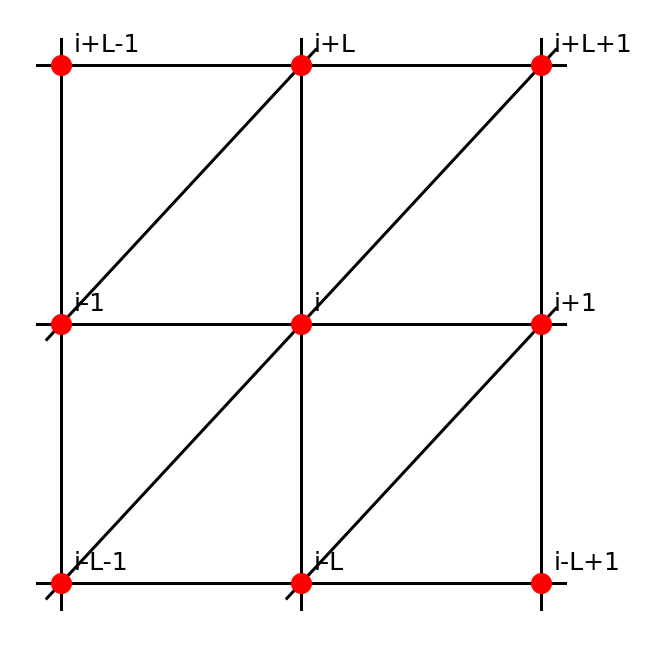
\includegraphics[width=0.3\textwidth]{TriLattice2.png}
    \caption{Связи узлов в квадратной (слева) и треугольной решёток (справа). 
	Узлы пронумерованы последовательно (слева на направо и снизу вверх), в одном ряду решётки L узлов.}
    \label{fig:lattices}
\end{figure}

Первая часть выпускной квалификационной работы посвящена исследованию \textit{локального координационного числа} мономеров блуждания
в виде долей узлов блуждания с фиксированным числом соседей \eqref{eq:n_i}.
Минимальное исследуемое число соседей в моделях блужданий без самопересечений - два, что соответствует внутреннему узлу одномерной цепочки с соседями в виде предыдующего и следующего в последовательности.
Максимальное исследуемое число соседей соответствует координационному числу рассматриваемой решётки $C_L$. 
Для каждого узла $u_i$ блуждания рассчитывается число его соседей $c_i$ \eqref{eq:c_i} и ведётся статистика узлов блуждания с таким же числом соседей.

\begin{equation}
\label{eq:c_i}
c_i = \sum_{\la u_i \textup{(fixed)}, j \ra} 1
\end{equation}

\begin{equation}
\label{eq:n_i}
n_k = \sum_{i=1}^{N-2}[c_i == k] / N
\end{equation}

Частный случаем локального координационного числа является атмосфера СБС - число незанятых мономерами блуждания узлов решётки вокруг конца блуждания \cite{owczarek2008scaling}.

\begin{equation}
\label{eq:atm}
a = C_L - c_{n-1},
\end{equation}

где $C_L$ - координационное число исследуемой решётки, а $c_{n-1}$ - число соседей конца блуждания

Определим два основных критических вида перехода, происходящих в моделях - конформационный и магнитный.
Конформационный переход разделяет состояние рыхлой цепочки (при высоких температурах / низкой силе взаимодействия) и плотной глобулы (при низких температурах / сильном взаимодействии ближайших узлов).
Для исследования конформационного перехода исследуется расстояние между концами блуждания $R^2_N$:
 
\begin{equation}
\label{eq:R2_base}
	R^2_N = (u_{N-1} - u_{0})^2
\end{equation}

Состояния отличаются шкалированием радиуса между концами блужданий $\la R^2_N \ra$ относительно длины цепочки $N$:
при больших длинах цепочки (N >> 1) радиус \eqref{eq:R2_base} шкалируется по степенному закону с поправками на конечный размер цепочки.

\begin{equation}
	\la R^2_N \ra = N^{2\nu}(C + ...)
\end{equation}

В качестве основной магнитной характеристики модели рассматривается набор средних намагниченностей нескольких порядков:

\begin{equation}
\label{eq:IsISAW_m2}
	m^{k} = (\sum_{i \in u} \sigma_i / N)^k
\end{equation} 

Для поиска точки магнитного перехода рассматривается зависимость кумулянта Биндера $U_4$ \eqref{eq:IsISAW_U4} от константы J.

\begin{equation}
\label{eq:IsISAW_U4}
	U_4 = 1 - \frac{\la m^4 \ra}{3 (\la m^2 \ra)^2}
\end{equation}

Для регулярной модели Изинга было доказано \cite{Binder1981_Ising}, 
что с ростом размеров решётки значение кумулянта сходится к 0 при парамагнетическом состоянии, 
и к 2/3, что соответствует ферромагнетическим свойствам модели.
В работе \cite{Binder1981_Ising} так же было обнаружено нетривиальное значение кумулянта, почти независящее от размеров решётки.
Значение константы J, при котором достигалась нетривиальная сходимость, являлось точкой магнитного перехода модели.
Таким образом, предполагается, что точкой магнитного перехода модели является 
точка пересечения графиков кумулянта $U_4$ при разных длинах цепочки.

Ниже представлены точки фазового перехода модели взаимодействующих блужданий и модели Изинга на СБС, ранее полученные в других работах (таблица \ref{tab:crits}), 
а так же полученные в рамках данной работы (таблица \ref{tab:res_crits}).

\begin{table}[h!]
    \centering
    \begin{tabular}{|c|c|c|}
        \hline
        lattice & Ising-ISAW & ISAW \\ \hline
        square & 0.8340(5)\cite{faizullina2021critical} &  0.6673(5)\cite{caracciolo2011geometrical} \\ \hline
        triangular & $-$ & 0.41(7) \cite{Privman1986}\\ \hline
        cubic & $0.5263 \pm 0.055$\cite{foster2021critical} & $0.2779 \pm 0.0041$\cite{Tesi1996} \\ \hline
    \end{tabular}
    \caption{Значения J критических точек фазового перехода модели Изинга на случайном блуждании (Ising-ISAW) и взаимодействующего полимера (ISAW) 
		на квадратной, треугольной и кубической решётках соответственно}
    \label{tab:crits}
\end{table}

\begin{table}[h!]
    \centering
    \begin{tabular}{|c|c|c|}
        \hline
        lattice & Ising-ISAW & ISAW \\ \hline
        triangular & 0.545(5) & 0.42(1)\\ \hline
    \end{tabular}
    \caption{Дополнение к таблице \ref{tab:crits}: результаты, полученные в рамках данной работы}
    \label{tab:res_crits}
\end{table}

Для симуляции моделей в несколькими степенями свобод применяются методы Монте-Карло.
Исследуемая модель Ising-ISAW уже рассматривалась ранее в работах \cite{Garel1999, Papale2018} задаче замороженного беспорядка - когда свойства модели исследовались генерацией спиновой подсистемы на уже сгенерированных конформациях.
В нашей работе исследуется задача динамического беспорядка, в которой генерируются одновременно и блуждания фиксированной длины N, и спиновые состояния на ней.
Для генерации движущихся конформаций фиксированной длины используется алгоритм на основе метода Червя \cite{Worm}, 
в то время как генерация состояний спиновой подсистемы проводится с помощью кластерного алгоритма Вольфа \cite{Wolff}.
Полное описание используемого метода моделирования описаны в работе \cite{faizullina2021critical}.


\section{Геометрические свойства модели Ising-ISAW с точки зрения числа соседей в узлах}

\subsection{Введение}

В данном разделе мы изучаем такое геометрическое свойство модели, как доли узлов с фиксированным числов соседей. У каждого узла можно определить число соседей или количество близких связей на смежных ячейках исследуемой решётки (см. левый рисунок \ref{fig:lattices}). Рассмотрим пример конформации на квадратной решётке на рисунке \ref{fig:example_bulk}. Чёрные точки соответствуют узлам с 2-мя соседями, а последовательность таких узлов подряд в конформации можно интерпретировать как "одномерный" участок. Узлы с тремя соседями расположены, как правило, на границах кластеров, и отображены на примере синими треугольниками, в то время как узлы с четырьмя соседями (красные квадраты) типичны для узлов в глубине кластера.

\begin{wrapfigure}{r}{0.25\textwidth}
    \centering
    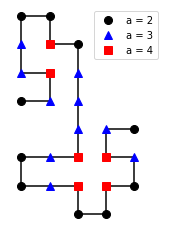
\includegraphics[width=0.24\textwidth, height=5cm]{update.png}
    \caption{Пример конформации на квадратной решётке с подсчётом соседей}
    \label{fig:example_bulk}
\end{wrapfigure}


Сначала, чтобы определить правильность алгоритма расчёта долей искомых узлов, были проведены симуляции Монте-Карло модели ISAW при J=0 на длинах N от 5 до 3600, а так же произведены расчёты вручную для цепочек малых длин - от 5 до 11. Результаты изображены на рисунке \ref{fig:ISAW_Bulk_J0} - разные типы расчётов полностью совпали, что говорит о правильности использумоего алгоритма.

\begin{figure}[]
    \centering
    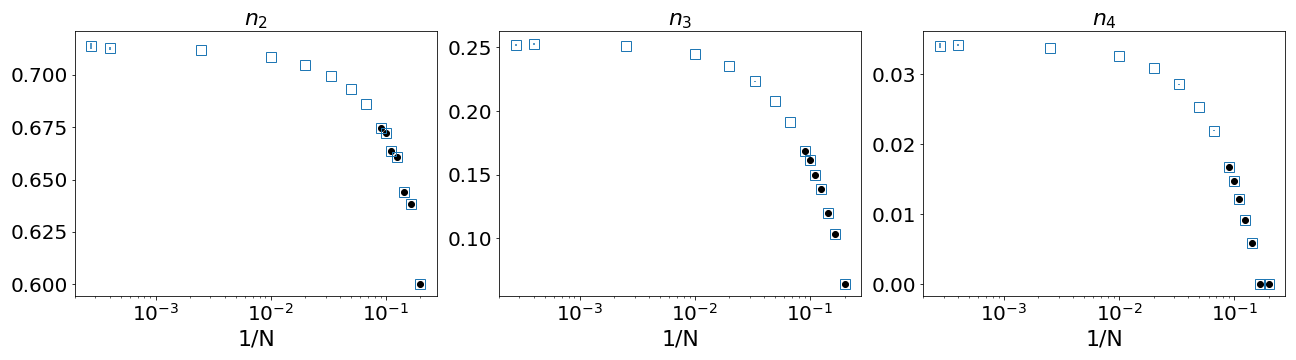
\includegraphics[width=0.95\textwidth]{ISAWJ0_Bulk2-4.png}
    \caption{Зависимостей средних долей узлов конформации с фиксированным числом соседей (от 2 до 4) модели ISAW при J=0 от обратной длины 1/N при длинах конформации N=5-3600. 
	Пустые квадраты - результаты симуляций Монте-Карло, черные точки - расчёты полученные путём полного перебора возможных конформаций\cite{web:sawRepos}}
    \label{fig:ISAW_Bulk_J0}
\end{figure}

\subsection{Особенности ранних результатов на квадратной решётке}

Мы провели симуляции Монте-Карло для долей узлов с фиксированным числом соседей для моделей Ising-ISAW и ISAW с зависимостью от значения константы взаимодействия J для длин N=1000, 2500, 3600, 4900. Результаты изображены на рисунке \ref{fig:Ising_vs_ISAW__2D_bulk}, а также опубликованы в работе \cite{faizullina2021critical}. 

\begin{figure}[h!]
    \centering
    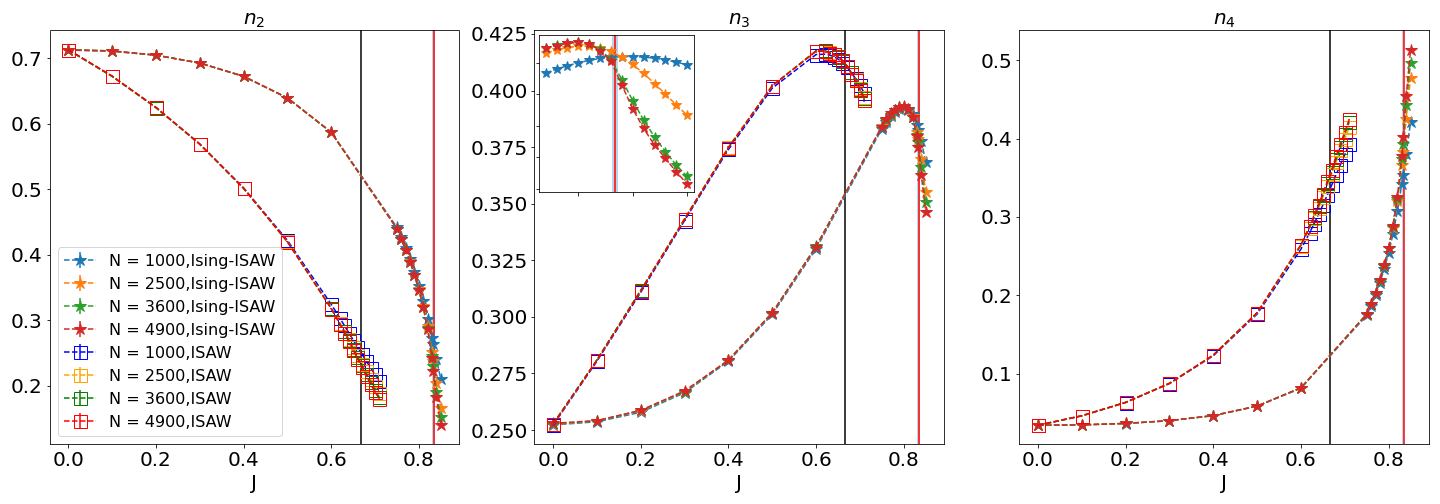
\includegraphics[width=0.95\textwidth]{bulk2-4_inset.png}
    \caption{Зависимость доли узлов конформации с двумя (слева), тремя (по центру) и четырьмя соседями (справа) у моделей Ising-ISAW (звезды) и ISAW на квадратной решётке от J. 
	Черной линией обозначена точка фазового перехода модели ISAW, красной - Ising-ISAW, на квадратной решётке (см. таблицу \ref{tab:crits}). 
	График взят из работы \cite{faizullina2021critical}}
    \label{fig:Ising_vs_ISAW__2D_bulk}
\end{figure}

На графиках \ref{fig:Ising_vs_ISAW__2D_bulk} примечательны значения в точке J=0 у графиков узлов с 2-мя (левый) и 3-мя (средний) соседями: было первоначальное предположение, что в пределе бесконечной длины конформации они будут равны 3/4 и 1/4 соответственно. Так же интересен вопрос универсальности данного свойства на других решётках: будут ли эти значения долей $n_{2}$ и $n_{3}$ при тех же условиях равны или хотя бы похожи в других решётках. 

\subsection{Сравнение модели Изинга и полимерной цепочки в решетках с 2-6 возможными соседями мономеров}

Рассмотрим средние доли узлов с фиксированным числом соседей в решётках, которые имеют от 2-х до 6-ти возможных соседей: в кубической, у которой 5-й и 6-й соседи мономера расположены в соседних плоскостях, и треугольной, где 5-й и 6-й сосед мономера лежат на диагонали, проходящей через данный узел (в данной решётке лишь одна плоскость, см. правый рисунок \ref{fig:lattices}).

График зависимости долей от константы взаимодействия J (используется в гамильтониане конформации по формуле \ref{eq:Ham}, однако в отличие от одномерного случая, где считаются связи между соседними по индексу узлами конформации, здесь считаются связи между узлами, лежащими на соседних ячейках исследуемой решётки) изображен на рисунке \ref{fig:Ising_vs_ISAW} - слева показаны результаты симуляций Монте-Карло на кубической решётке, справа - на треугольной решётке. Цвета графиков соответствуют длинам цепочек - N=100 зелёные, 300 синие, 600 красные и 1200 фиолетовые. Число шагов симуляций - от $10^{10}$ вдали от пиков до $10^{12}$ в районе пиков графиков. Вертикальными линиями отмечены точки критического перехода: 

\begin{table}[h!]
    \centering
    \begin{tabular}{|c|c|c|}
        \hline
        lattice & Ising-ISAW & ISAW \\ \hline
        square & 0.8340(5)\cite{faizullina2021critical} &  0.6673(5)\cite{caracciolo2011geometrical} \\ \hline
        triangular & Unknown & 0.41(7) \cite{Privman1986}\\ \hline
        cubic & $0.5263 \pm 0.055$\cite{foster2021critical} & $0.2779 \pm 0.0041$\cite{Tesi1996} \\ \hline
    \end{tabular}
    \caption{Значения J критических точек фазового перехода модели Изинга на случайном блуждании (Ising-ISAW) и гомополимера (ISAW) на квадратной, треугольной и кубической решётка соответственно (в порядке строк)}
    \label{tab:crits}
\end{table}

Результаты симуляций модели ISAW отмечены пустыми квадратами, а модели Ising-ISAW - звёздами. Примечательно, что графики зависимости долей от J данной модели значительно плавнее, чем у модели Изинга на случайном блуждании, а так же процессы уплотнения конформаций (когда доли $n_{2}$ и $n_{3}$ уменьшаются, а доли узлов с большим числом соседей увеличивается) начинаются раньше, пропорционально значению точки перехода $J_{c}$. Последнее, скорее всего, связано с тем, что точка перехода модели ISAW меньше, чем у Ising-ISAW (для кубической это известно, для треугольной просто предположение). Возможно, что при масштабировании левой части графиков кубической решетки относительно $J_{c}$ (то есть, от $0*J_{c}$ до $1*J_{c}$), мы бы получили примерно одинаковые графики.

В то же время, предельные значения у данных моделей совпадают - графики одинанаковых длин и решёток разных моделей исходят из одной точки при J=0 (что логично, ведь при J=0 поведение Ising-ISAW соответствует ISAW) и приходят в одну точку при J=1.

Данные модели Ising-ISAW в свою очередь отмечены на графике \ref{fig:Ising_vs_ISAW} звездочками. Стоит отметить, что при прохождении точки перехода в кубической решётке, графики долей узлов с любым числов соседей словно претерпевают скачок, усиливающийся с ростом длины цепочки, в отличие от треугольной решётки, где процесс непрерывен.

Говоря о свойствах Ising-ISAW кубической решётки, необходимо подчеркнуть, что в на графике $\la n_{3} \ra$ мы видим похожее поведение в J=0 - значение довольно близко к 0.25, стоит проверить предел значения доли узлов с 3-мя соседями в J=0 при бесконечной длине и характер приближения к нему, если таковой имеется. Значение $\la n_{2} \ra$ при J=0 визуально отличается от предполаемого $3/4$. В следующих разделах мы рассмотрим развитие значения долей $\la n_{2-6} \ra$ в точке J=0 (где модели ISAW и Ising-ISAW ведут себя идентично с обычным невзаимоидействующим блужданием SAW) на разных решётках на пределе бесконечной длины.

\begin{figure}
    \centering
    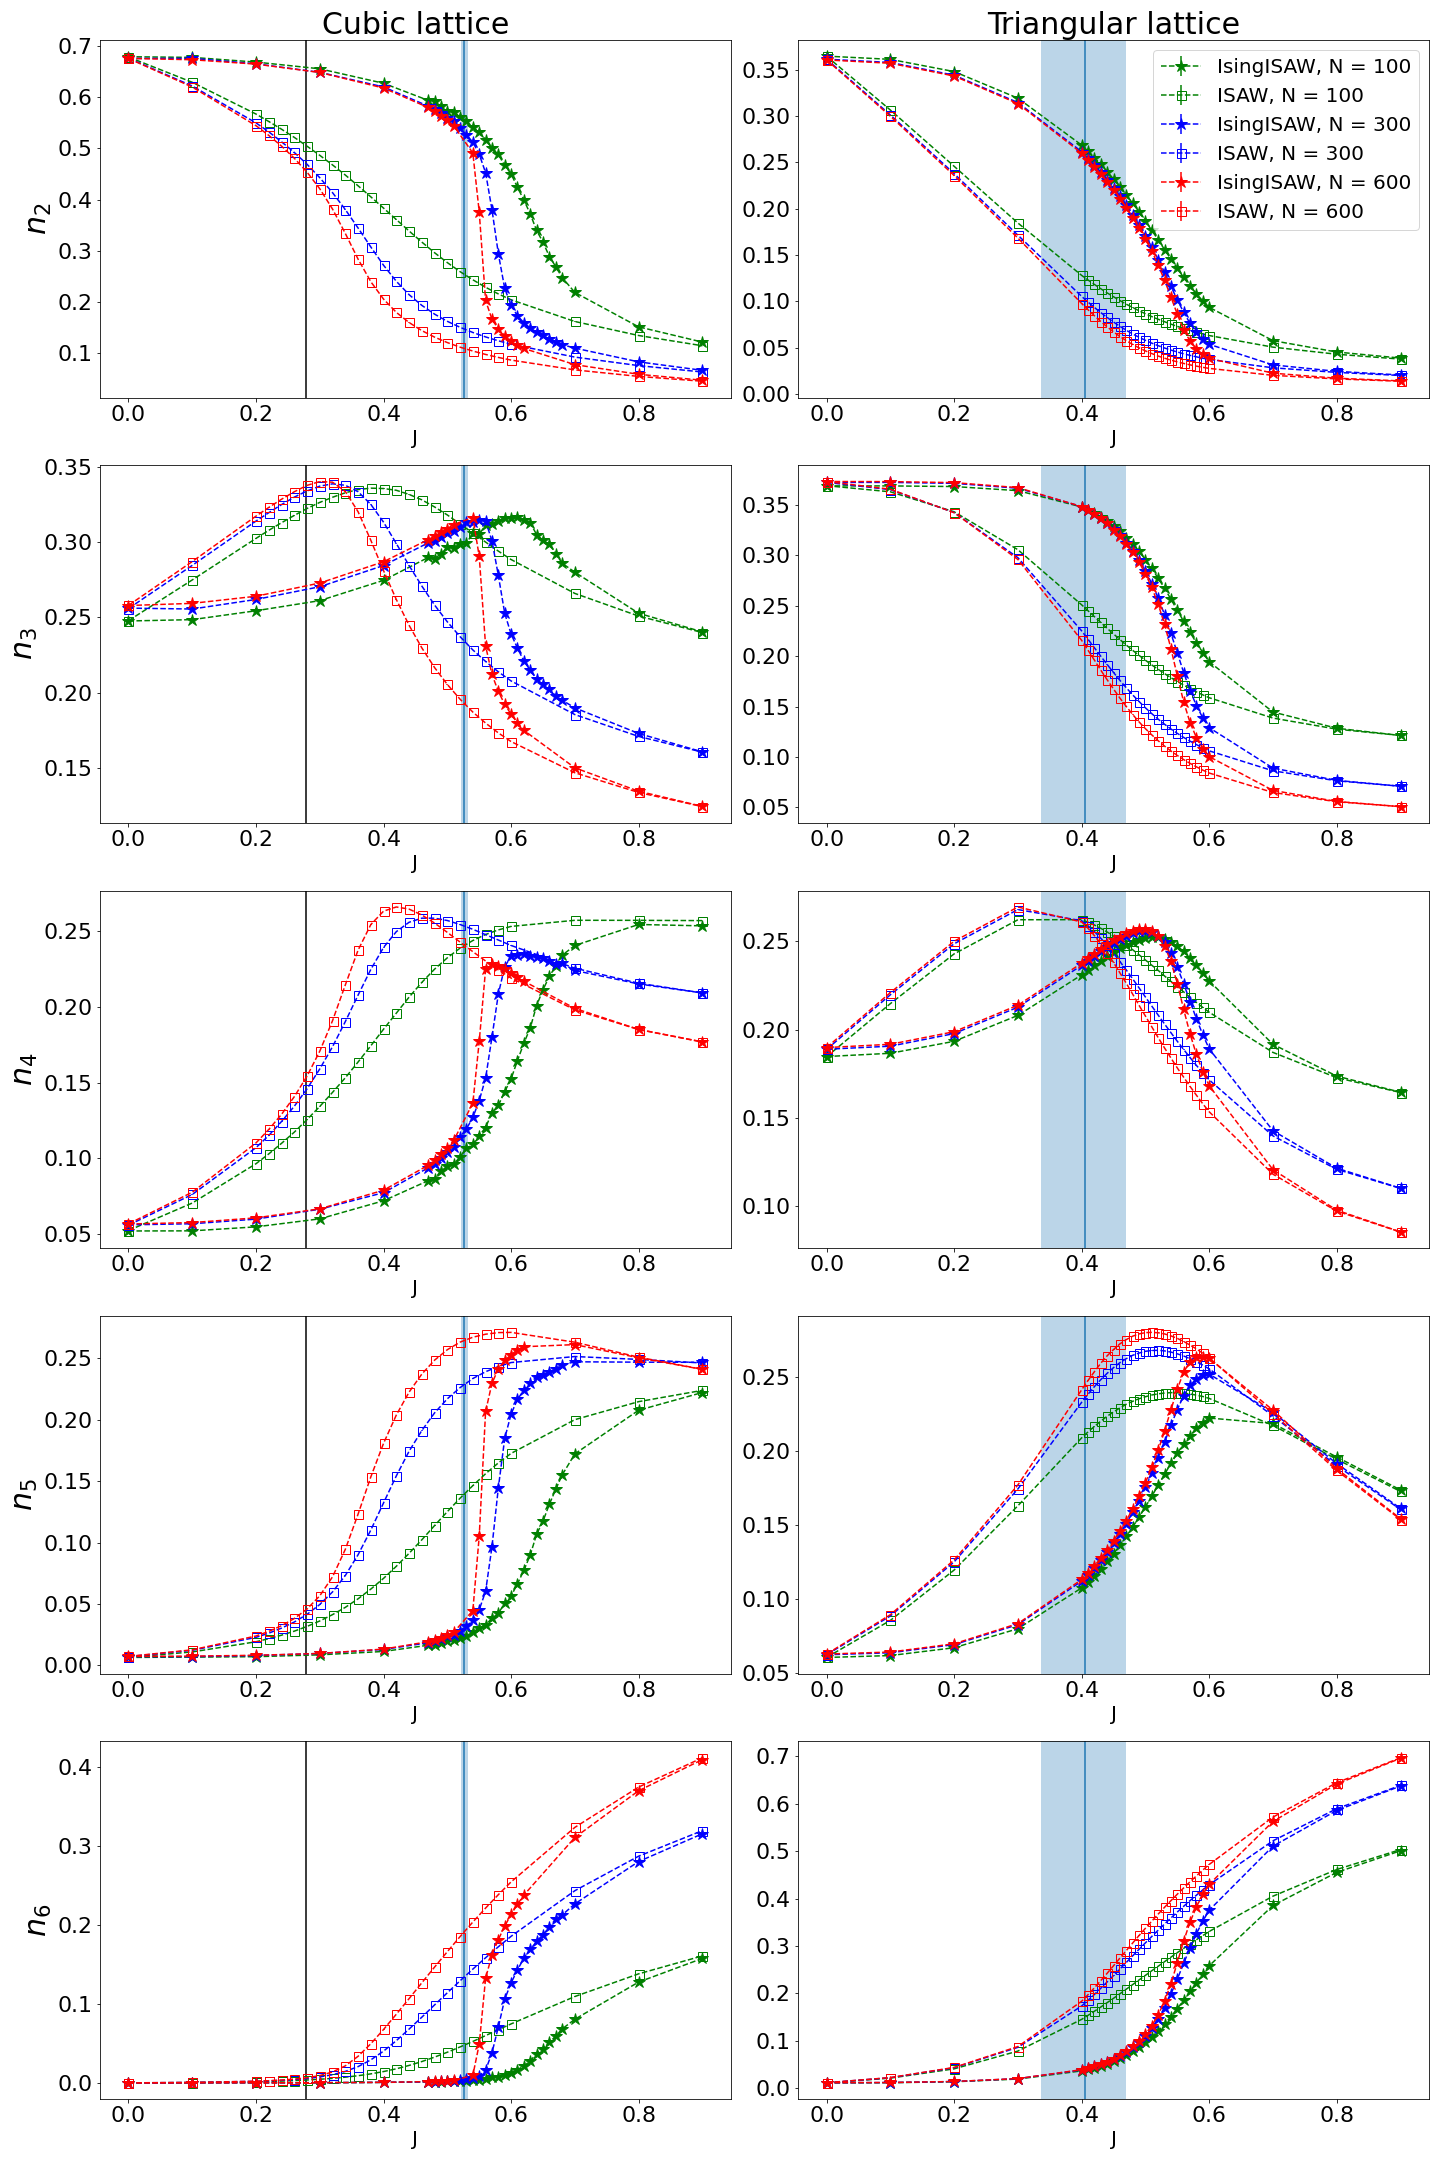
\includegraphics[width=0.95\textwidth, height=21.5cm]{Ising_vs_ISAW.png}
    \caption{Зависимость доли узлов моделей Ising-ISAW (звезды) и ISAW (квадраты) на кубической (слева) и треугольной решётках (справа) с 2-6 соседями (сверху вниз) от $J$ c длинами N = 100 (зеленые), 300 (красные), 600 (синие) и 1200 (фиолетовые). Вертикальные линии отмечают точки фазового перехода моделей \ref{tab:crits}}
    \label{fig:Ising_vs_ISAW}
\end{figure}

\newpage

\subsection{Алгоритм исследования характера зависимости значения долей узлов от длины при J=0}

Здесь рассматривается способ определения характера зависимости у графиков долей узлов с фиксированным числов соседей при J=0. Для примера взят случай $n_{2}$ у квадратной решётки модели Ising-ISAW. Первоначально рассматривается три возможных способа апроксимации результатов, варьирующихся зависимостью от обратной длины конформации $x = 1/N$:

\begin{enumerate}
    \item Линейная апроксимация 
    \begin{equation}
    \label{eq:linreg}
        y = a x + b
    \end{equation}
    \item Лог-линейная или экспоненциальная апроксимация 
    \begin{equation}
        y = b \exp{(a x)} + c 
    \end{equation}
    \item Степенная или лог-лог апроксимация
    \begin{equation}
        y = b x^{a} + c
    \end{equation}
\end{enumerate}

Чтобы гарантировано получить результат использовалась функция linregress из пакета scipy.stats, поэтому на данном этапе погрешностью результатов симуляций мы временно пренебрегаем. Так же, чтобы показать нагляднее характер апроксимации, графики соответсвующих способов фитирования будут рассмотрены в том же масштабе - линейный в линейном, экспоненциальный в лог-линейном, степенном в лог-лог-масштабе - таким образом графики фитов будут линейными. Результаты апроксимаций в порядке, изложенном в списке выше, изображены на рисунках \ref{fig:square_scale_full} и \ref{fig:square_scale_limited} - в левом столбце апроксимации записаны для данных цепочек с длинами от 100 до 4900, в правом - длины от 250 до 4900, чтобы оценить поведение модели на больших длинах, следовательно, ближе к нулю.

\begin{figure}[h!]

\begin{subfigure}{0.49\textwidth}
    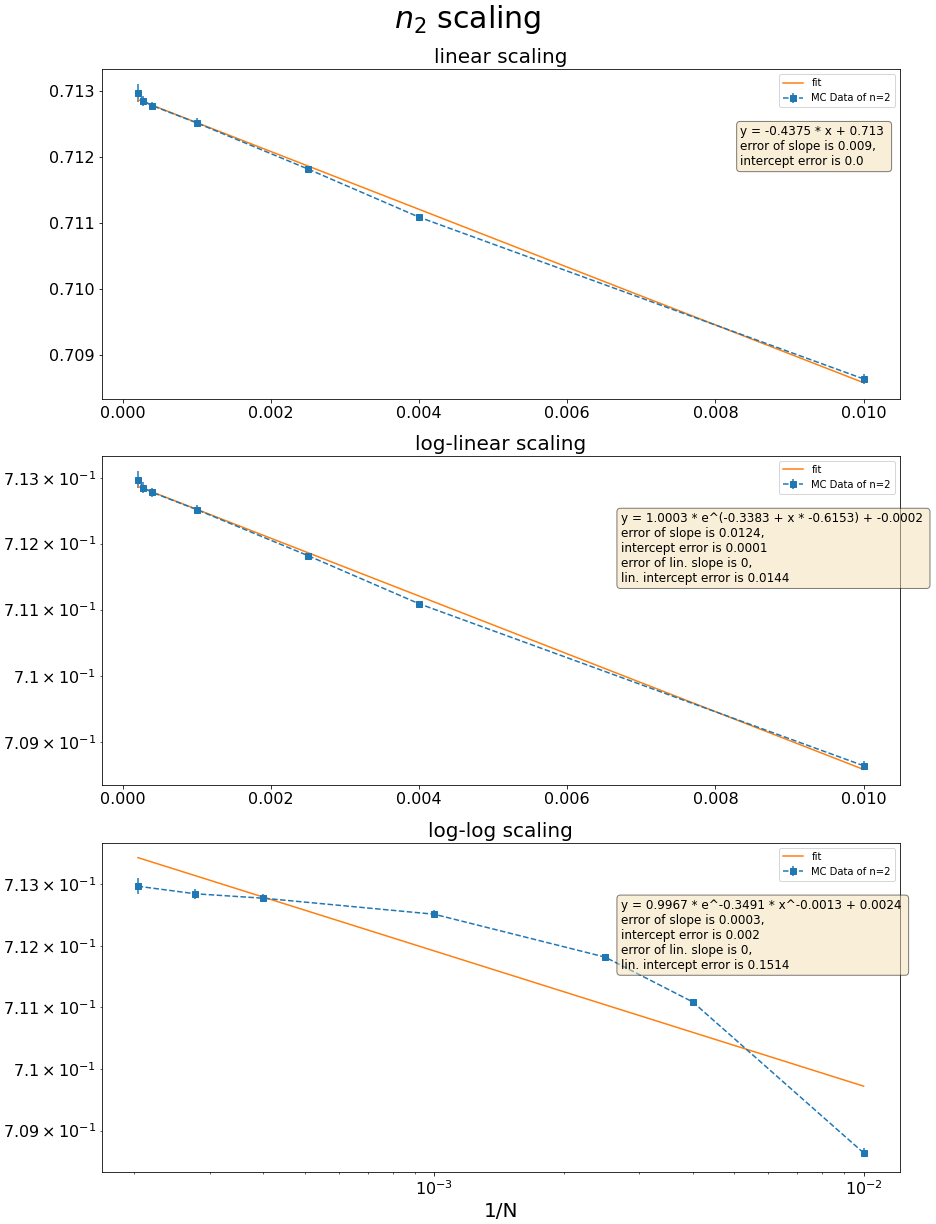
\includegraphics[width=\textwidth]{square_n2_scaling.png}
    \caption{}
    \label{fig:square_scale_full}
\end{subfigure}
\hfill
\begin{subfigure}{0.49\textwidth}
    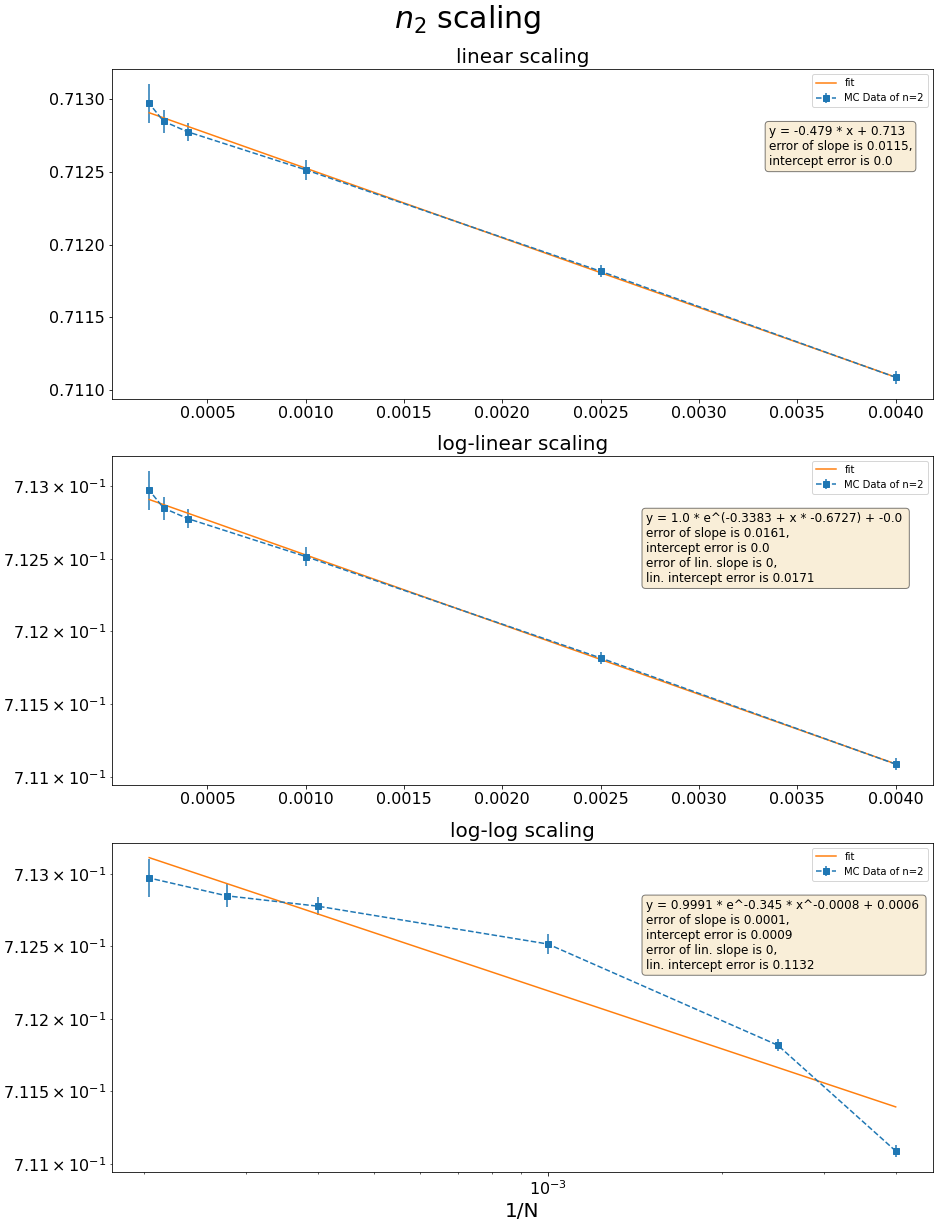
\includegraphics[width=\textwidth]{square_n2_scaling2.png}
    \caption{}
    \label{fig:square_scale_limited}
\end{subfigure}
\caption{Результаты апроксимации (оранжевая линия) данных Монте-Карло о долей узлов с двумя соседями $n_2$ модели Ising-ISAW на квадратной решётке (синие точки) различными способами на диапазоне длин 100-4900 (a) и 250-4900 (b)}
\end{figure}

Графики на рисунках \ref{fig:square_scale_full} и \ref{fig:square_scale_limited} показывают, что в данном случае экспоненциальная апроксимация ведёт себя как линейная (что логично вблизи нуля), поэтому можно рассматривать вместо первых двух только линейную. С другой стороны, степенная функция совсем не совпадает с графиком результатов. Более того, значение степени функции-фита настолько мало, что итоговая функция больше похожа на константную прямую.

Таким образом, в данном случае определён линейный характер зависимости. Теперь, чтобы оценить качество приближения при рассмотрении точек всё ближе и ближе к нулю, оценим ошибку фитирования - теперь мы можем использовать функцию curve-fit из пакета scipy.optimize.

\begin{table}[h]
    \centering
    \begin{tabular}{|c|c|c|} \hline
        N & a & b  \\ \hline
        100-4900 & -0.44(1) & 0.71292(4) \\ \hline
        250-4900 & -0.473(6) & 0.71299(2) \\ \hline
        400-4900 & -0.47(1) & 0.71298(2) \\ \hline
        1000-4900 & -0.48(6) & 0.71299(4) \\ \hline
    \end{tabular}
    \caption{Значения и погрешности коэффициентов линейного фитирования \eqref{eq:linreg} зависимости долей узлов с 2-мя соседями на квадратной решётке модели Ising-ISAW при J=0 от исследуемого интервала длин}
    \label{tab:a_b_n2_square}
\end{table}

Результаты использования других диапазонов точек на таблице \ref{tab:a_b_n2_square} показывают, что наиболее оптимальный фит (с наименьшей ошибкой) достигается при выборе точек от 250 до 4900. Это можно объяснить тем, что при выборе точек большего диапазона линейный характер будет выражен слабее, а при выборе точек меньшего диапазона количество рассматриваемых данных уменьшается, что приводит к росту ошибки (недостаточно статистики). Подобная операция была выполнена и для других чисел соседей и решёток (более подробные графики см. в Bulk2-6.ipynb в разделе "Расчёты .ipynb" \cite{web:ProjectMagnetRepos}), результаты представлены в следующем разделе в виде графиков для узлов с 2-мя и 3-мя соседями и в виде таблицы коэффициентов линейного фитирования \eqref{eq:linreg} без графиков. 

Результаты линейного фитирования при выборе разной наименьшей рассматриваемой длины можно увидеть на таблицах \ref{tab:n24_fit_coeff_100} и \ref{tab:n24_fit_coeff_200}. По погрешностях на первых строках обеих таблиц понятно, что оптимальным диапазоном будет 250-4900. Для 3-4D-гиперкубических решёток так же заметно (по погрешностям соответствующих строк), что отбрасывание длины N=100 из рассмартиваемых улучшило точность результатов. Единственное исключение - треугольная решётка: на ней линейный характер результатов настолько заметен, что при отбрасывании наименьшей длины N=100 ошибка увеличивается (недостаточность статистики стала сильнее, а ''линейность'' не изменилась).

\newpage

\subsection{Сравнение геометрических свойств модели Изинга на треугольной решётке с квадратной в J=0}

\begin{figure}
    \centering
    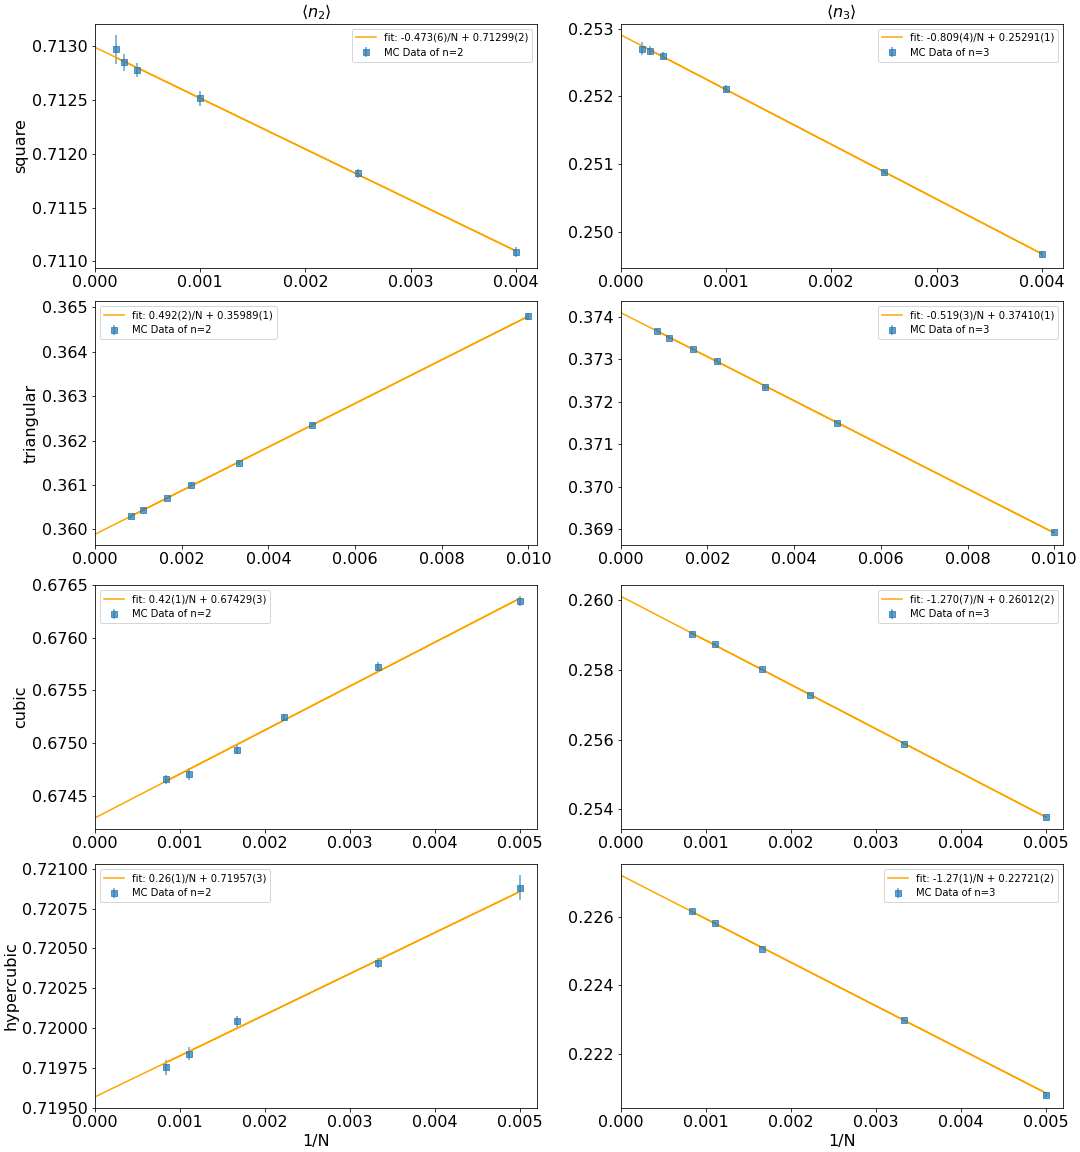
\includegraphics[width=0.95\textwidth]{n23_linear.png}
    \caption{Зависимость средней доли узлов с 2-мя соседями (слева) и 3-мя (справа) от обратной длины 1/N в модели Изинга на случайном блуждании на квадратной, треугольной, кубической и гиперкубической (сверху вниз). Синие точки описывают результаты симуляций Монте-Карло, оранжевая линия - график линейной апроксимации результатов, ошибки рассчитаны с учётом погрешностей полученных данных. Коэфициенты и диапазоны длин рассматриваемых данных записаны в таблице \ref{tab:n24_fit_coeff}}
    \label{fig:all_n23_bulk}
\end{figure}

На графике \ref{fig:all_n23_bulk} наглядно показано сравнение приближений долей "одномерных" участков (то есть, долей мономеров с двумя соседями) и узлов с тремя соседями в цепочках на квадратной, треугольной, кубической и гиперкубической решётках. Для расчётов долей на треугольной решётке были использованы длины 100-1200, для квадратной - 250-4900, для кубической и гиперкубической - 200-1200. Фитирование долей треугольной решётки имеет отчётливый линейный характер, даже в приближении на короткие длины. Линейность долей прямоугольных решёток всех размерностей также подтверждается (с учётом погрешности расчётов с наибольшей длиной). 

\begin{table}[h]
    \centering
    \begin{tabular}{|c|c|c|c|c|c|c|} \hline
         & \multicolumn{2}{|c|}{$\la n_{2} \ra$} & \multicolumn{2}{|c|}{$\la n_{3} \ra$} & \multicolumn{2}{|c|}{$\la n_{4} \ra$}\\ \hline
         Lattice & a & b & a & b  & a & b  \\ \hline
        Square & -0.44(1) & 0.71291(4) & -0.843(8) & 0.25297(3) &  -0.154(3) & 0.03412(1)  \\ \hline
        Triangular & 0.492(2) & 0.35989(1) & -0.519(3) & 0.37410(1) & -0.609(4) & 0.19080(1)  \\ \hline
        Cubic & 0.37(2) & 0.67440(7) &  -1.24(1) & 0.26005(5) & -0.525(5) & 0.05758(1) \\ \hline
        Hypercubic & 0.15(2) & 0.71978(9) & -1.20(1) & 0.22080(6) & -0.468(5) & 0.04589(2)\\ \hline
    \end{tabular}
    \caption{Коэффициенты прямых, полученные линейным фитированием \eqref{eq:linreg} данных симуляций Монтекарло по долям улов с 2-4 соседями из рисунков \ref{fig:all_n23_bulk} для длин N от 100 до 4900 (для квадратной) и 1200 (для остальных решёток)}
    \label{tab:n24_fit_coeff_100}
\end{table}

\begin{table}[h]
    \centering
    \begin{tabular}{|c|c|c|c|c|c|c|} \hline
         & \multicolumn{2}{|c|}{$\la n_{2} \ra$} & \multicolumn{2}{|c|}{$\la n_{3} \ra$} & \multicolumn{2}{|c|}{$\la n_{4} \ra$}\\ \hline
         Lattice & a & b & a & b  & a & b  \\ \hline
        Square & -0.473(6) & 0.71299(1) & -0.809(3) & 0.25291(1) &  -0.145(4) & 0.03410(1)  \\ \hline
        Triangular & 0.491(3) & 0.35989(1) & -0.523(6) & 0.37411(1) & -0.603(8) & 0.19079(2)  \\ \hline
        Cubic & 0.418(1) & 0.67429(3) &  -1.27(1) & 0.26012(2) & -0.538(4) & 0.05761(1) \\ \hline
        Hypercubic & 0.26(1) & 0.71958(3) & -1.27(1) & 0.22720(2) & -0.494(6) & 0.04596(1)\\ \hline
    \end{tabular}
    \caption{Коэффициенты прямых, полученные линейным фитированием \eqref{eq:linreg} данных симуляций Монтекарло по долям улов с 2-4 соседями из рисунков \ref{fig:all_n23_bulk} для длин N от 250 до 4900 (для квадратной) и от 200 до 1200 (для остальных решёток)}
    \label{tab:n24_fit_coeff_200}
\end{table}

\begin{table}[h]
    \centering
    \begin{tabular}{|c|c|c|c|c|c|c|c|c|c|} \hline
         & \multicolumn{3}{|c|}{$\la n_{2} \ra$} & \multicolumn{3}{|c|}{$\la n_{3} \ra$} & \multicolumn{3}{|c|}{$\la n_{4} \ra$}\\ \hline
         Lattice & a & b & N & a & b & N & a & b & N \\ \hline
        Square & -0.473(6) & 0.71299(2) & 250-4900 & -0.809(4) & 0.25291(1) & 250-4900 & -0.145(4) & 0.03410(1) & 250-4900  \\ \hline
        Triangular & 0.492(2) & 0.35989(1) & 100-1200 & -0.519(3) & 0.37410(1) & 100-1200 & -0.609(4) & 0.19080(1) & 100-1200 \\ \hline
        Cubic & 0.42(1) & 0.67429(3) & 200-1200 & -1.270(7) & 0.26012(2) & 200-1200 & -0.538(4) & 0.05671(1) & 200-1200 \\ \hline
        Hypercubic & 0.26(1) & 0.71957(3) & 200-1200 & -1.27(1) & 0.22721(2) & 200-1200 & -0.494(6) & 0.04595(1) & 200-1200\\ \hline
    \end{tabular}
    \caption{Коэффициенты прямых, полученные линейным фитированием \eqref{eq:linreg} данных симуляций Монтекарло по долям улов с 2-4 соседями из рисунков \ref{fig:all_n23_bulk} - наилучшие приближения с подбором диапазона длин для каждого графика (в столбце N)}
    \label{tab:n24_fit_coeff}
\end{table}

Из таблицы \ref{tab:n24_fit_coeff} по первым двум строках, отображающим данные о прямых-фитов квадратной и треугольной решётки соответствено, сходства между одномерием треугольной и квадратной решётки с точки зрения коэфициентов фитирования $a$ и $b$ \eqref{eq:linreg} почти не наблюдается - они имеют как разные значения свободных членов, так и значения и даже (в случае 2-х соседей) знаки коэффициента наклона, разница который значительно превышает погрешность фита. 

Значение свободного члена $b$ для $\la n_{2} \ra$, то есть предела значения долей при бесконечной длине цепочки, у квадратной и треугольной решётки (первый блок первых двух строк таблицы \ref{tab:n24_fit_coeff}) отличается почти в два раза: $0.71299(2)$ и $0.35989(1)$ (что логично, ведь в треугольной решётке диагональные ячейки так же считаются соседними, поэтому половина поворотов конформации добавит соседей).



\subsection{Сравнение геометрических свойств модели Изинга на решётках с большим числом соседей в J=0}

\begin{table}[]
    \centering
    \begin{tabular}{|c|c|c|c|c|c|c|} \hline
         & \multicolumn{3}{|c|}{$\la n_{5} \ra$} & \multicolumn{3}{|c|}{$\la n_{6} \ra$}  \\ \hline
        Lattice & a & b & N & a & b & N \\ \hline 
        Triangular & -0.274(2) & 0.063145(6) & 100-1200 & -0.055(1) & 0.012081(2) & 100-1200\\ \hline
        Cubic & -0.100(2) & 0.007536(4) & 200-1200 & -0.0074(2) & 0.000452(1) & 200-1200 \\ \hline
        Hypercubic & -0.102(2) & 0.00658(1) & 200-1200 & -0.0140(3) & 0.000659(1) & 200-1200\\ \hline
    \end{tabular}
    \caption{Коэффициенты прямых, полученные линейным фитированием \eqref{eq:linreg} данных симуляций Монтекарло по долям улов с 5-6 соседями}
    \label{tab:n56_fit_coeff}
\end{table}

\begin{table}[]
    \centering
    \begin{tabular}{|c|c|c|c|c|c|c|} \hline
         & \multicolumn{3}{|c|}{$\la n_{7} \ra$} & \multicolumn{3}{|c|}{$\la n_{8} \ra$}  \\ \hline
        Lattice & a & b & N & a & b & N \\ \hline 
        Hypercubic & -0.0011(1) & 0.0000420(3) & 200-1200 & -0.000024(35) & 0.0000010(1) & 200-1200\\ \hline
    \end{tabular}
    \caption{Коэффициенты прямых, полученные линейным фитированием \eqref{eq:linreg} данных симуляций Монтекарло по долям улов с 7-8 соседями}
    \label{tab:n78_fit_coeff}
\end{table}

Здесь мы сравниваем линейное фитирование результатов симуляций Монте-Карло треугольной решётки с кубической, имеющей такое же количество возможных соседей, а так же результаты для гиперкубической решётки в J=0. Коэффициенты линейного фитирования \eqref{eq:linreg} отображены в таблицах \ref{tab:n24_fit_coeff} и \ref{tab:n56_fit_coeff}: поскольку в таких условиях плотность конформаций минимальна, доля узлов с 7 и 8 соседей в конформациях на гиперкубической решётке почти нулевая, что видно по таблице \ref{tab:n78_fit_coeff}, поэтому мы рассматриваем число соседей лишь от 2 до 6. 

Рассматривая средние строки таблицы \ref{tab:n24_fit_coeff}, где записаны коэффициенты прямых фитирования для $n_{2}$ и $n_{3}$ треугольной и кубической решётки соответственно, а так же средние графики на рисунке \ref{fig:all_n23_bulk}, мы видим примерно ту же ситуацию как и в случае сравнения треугольной с квадратной - кубическая решётка на графике \ref{fig:all_n23_bulk} показывает почти чёткий линейный характер приближения в пределах погрешности наибольших длин (для n=3 линейно видна значительно лучше), но ни коэффициенты наклона $a$, ни значения свободных членов $b$ не имеют никакого сходства. Единственное отличие от сравнения с квадратной решёткой - графики соответствующих долей треугольной, кубической и гиперкубической решёток имеют одинаковое поведение с точки зрения знака наклона, что действительно и для долей узлов с больший числом соседей. Можно утверждать, что треугольная решётка с точки зрения поведения доли одномерных участок больше похожа на кубическую решётку, нежели квадратную, однако точной численной универсальности (например, почти равных в пределах погрешности коэффициентов) поведения доли "одномерных" участков между ними при бесконечно больших длинах конформации не обнаружена.

Единственная пара коэффициентов, которая оказалась равна в пределах погрешности, являются коэффициенты наклона у линейного фитирования $a$ \eqref{eq:linreg} для долей узлов с 3-мя соседями $\la n_{3} \ra$ у кубической и гиперкубической решёток (см. таблицу \ref{tab:n24_fit_coeff}).


\subsection{Число соседей и атмосферы блужданий}
\label{sec:Prellberg}

В статье \cite{owczarek2008scaling} в пространстве невзаимодействующих случайных блужданий без самопересечений было рассмотрено так свойство конформации, как "атмосфера" - количество возможных направлений для удлинения цепочки длины N или количество возможных N+1-х узлов.

Мы предполагаем, что данное свойство имеет связь с числом соседей при рассмотрении процесса удлинения цепочки и такие величины, как доля узлов цепочки $\la n_{i} \ra$ с фиксированным числом соседей и вероятность конформации иметь атмосферу $k$ - $p^{(k)}$ - по-разному описывают одно и то же поведение цепочек с точки зрения их плотности.

\begin{figure}
    \centering
    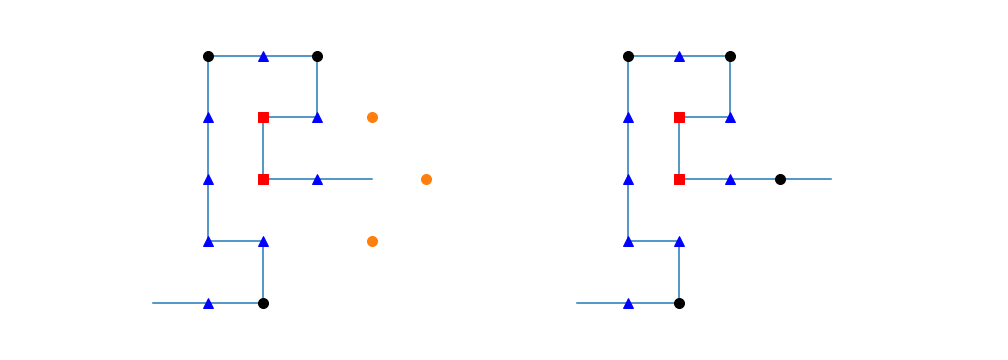
\includegraphics[width=0.5\textwidth]{Atmos_to_neibors_p3.png}
    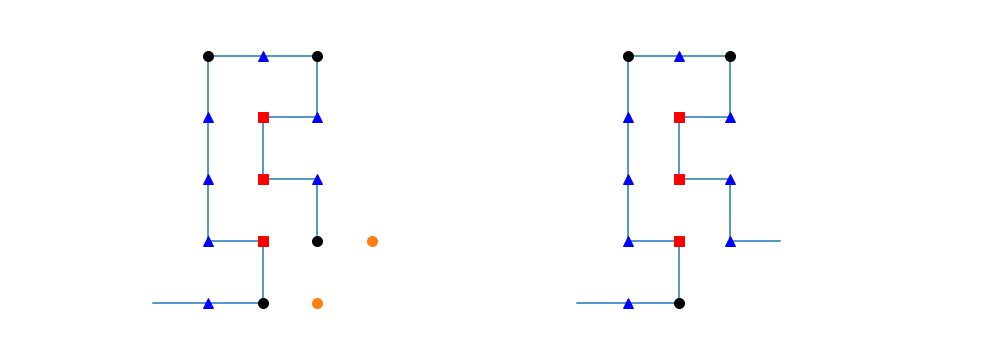
\includegraphics[width=0.5\textwidth]{Atmos_to_neibors_p2.png}
    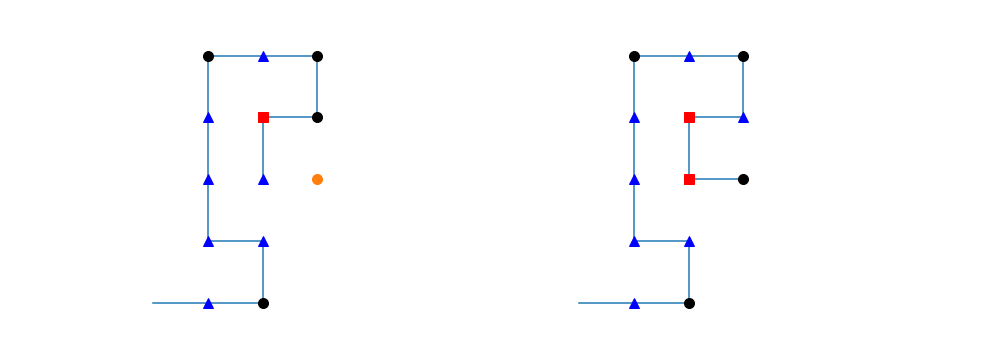
\includegraphics[width=0.5\textwidth]{Atmos_to_neibors_p1.png}
    \caption{Пример удлинения цепочки на квадратной решётке с атмосферой 3,2,1 (сверху вниз): слева изображена конформация до удлинения, справа - после, возможные способы добавить новый узел отмечены оранжевым, разметка узлов по количеству соседей соответствует рисунку \ref{fig:example_bulk}}
    \label{fig:atmos_neighs}
\end{figure}

Рассмотрим верхний рисунок \ref{fig:atmos_neighs}: если конец цепочки длины N (назовём его "N-ым узлом") имеет атмосферу три (три оранжевые точки вокруг правого конца), то при добавлении нового N+1-го узла N-й будет иметь два соседа: N-1-й и N+1-й узлы (бывший правый конец стал черной точкой). 

Так же при атмосфере 2 - как на среднем рисунке \ref{fig:atmos_neighs} - когда, уже имея два соседа (черная конечная точка) и две возможности для удлинения, N-ый узел при удлинении будет иметь 3 соседа (треугольник в том же месте на правой половине). 

И наконец, при атмосфере 1 (последний рисунок \ref{fig:atmos_neighs}) удлинение цепочки единственным возможным способом (одна оранжевая точка) приведёт к тому, что старый конец цепочки будет иметь 4 соседа (красный квадрат вместо треугольника). Примеры таких явлений можно увидеть на рисунке \ref{fig:atmos_neighs}. Очевидно, что случай удлинения при атмосфере 0 рассмореть невозможно, и провести аналогию с соседями нельзя.

Подобная интерпретация данных свойств в контексте удлинения цепочки показывает, что событие "цепочка длины N имеет атмосферу 3/2/1" при удлинении однозначно перехоходит к состоянию "N-й узел цепочки (теперь предпоследний) имеет 2/3/4 соседа" соответственно.

С другой стороны, подобная интерпретация атмосферы Преллберга не учитывает перерасчёт соседей у других узлов после удлинения цепочки - так, на примере атмосферы 1 (на нижнем рисунке \ref{fig:atmos_neighs}) видно, что у одного из узлов, кроме конечного (бывшая черная точка справа), так же увеличилось число соседей (с 2-х до 3-х), тем самым она стала поверхностным узлом (синим треугольником в том же месте на правой половине).

Проведём сравнение долей узлов в фикс. числом соседей в модели Ising-ISAW при J=0 и вероятность конформации модели невзаимодействующего блуждания иметь атмосферу k в пределе на бесконечно большую длину на квадратной решётке. 

\begin{table}[h]
    \centering
    \begin{tabular}{|c|c|c|c|}
    \hline
    k & $p^{(k)}$ & i & $b(\la n_{i} \ra)$ \\ \hline
    3 & 0.711 14(3) & 2 & $0.71299(2)$ \\ \hline
    2 & 0.225 00(2) & 3 & $0.25291(1)$ \\ \hline
    1 & 0.054 76(1) & 4 & $0.03410(1)$\\ \hline
    0 & 0.009 096(4) & - & - \\ \hline
    \end{tabular}
    \caption{Сравнение свободных членов линейных приближений вероятностей у конформации иметь n-ю атмосферу (слева) и долей мономеров с i соседями (справа) в зависимости от обратной длины конформации 1/N}
    \label{tab:Prellb_Compare}
\end{table}

На таблице \ref{tab:Prellb_Compare} слева изображены значения свободных членов графика зависимости вероятности гомополимерной цепочки иметь атмосферу k в статье \cite{owczarek2008scaling}, то есть вероятность, что второй конец цепочки бесконечно большой длины N имеет k возможных направления для удлинения и следовательно, k возможных узлов, которые могут стать новым узлом в цепочке. Справа изображены значения свободных членов приближений графиков долей узлов с i соседями. Хотя все значения отличаются больше чем на погрешность расчётов, однако нельзя не заметить довольно близкое сходство $p^{(3)}$ и свободного члена $\la n_{2} \ra$, хотя сами приближения имеют противоположные по знаку наклоны. 

В частной переписке с автором статьи была предложена следующая коррекция результатов \cite{web:PrellbergPrivate}: поскольку мы рассматриваем состояние при котором удлинения точно произойдёт, то сравнивать необходимо именно условные вероятности вида P({цепочка имеет атмосферу k | удлинение возможно}) = P({цепочка имеет атмосферу k}) / P({цепочка имеет положительную атмосферу}):

\begin{equation*}
    p^{(1/2/3)'} = p^{(1/2/3)} / (p^{(1)} + p^{(2)} + p^{(3)})
\end{equation*}

Рассмотрим такую ''приведённую'' вероятность атмосфер и сравним с результатами для долей соседей.

\begin{table}[h]
    \centering
    \begin{tabular}{|c|c|c|c|}
    \hline
    k & $p^{(k)'}$ & i & $b(\la n_{i} \ra)$ \\ \hline
    3 & 0.7177 & 2 & $0.71299(2)$ \\ \hline
    2 & 0.2271 & 3 & $0.25291(1)$ \\ \hline
    1 & 0.0553 & 4 & $0.03410(1)$\\ \hline
    \end{tabular}
    \caption{Вероятности у конформации иметь k-ю атмосферу (слева) и долей мономеров с i соседями (справа) в пределе бесконечной длины в случае гарантированно возможного удлинения}
    \label{tab:Prellb_Compare2}
\end{table}

Разница между $p^{(3)'}$ и $(\la n_{2} \ra)$ увеличилась. Остальные величины так же не удалось приравнять в пределах погрешности, что говорит о том, что величины обозначают несколько разные поведения модели.




\section{Введение}
\label{sec:neigh}

В рамкам дипломной работы "Магнитные и геометрические свойства модели Изинга на случайных блужданиях на решетке" 
в качестве завершения исследования поведения долей узлов с фиксированным числом соседей рассмотрим модель простого случайного блуждания (далее Random\_Walk или RW) на квадратной решётке. 
В модели RW отсутствует ограничение самопересечений, и, следовательно, есть возможность попадания в ранее занятые узлы решётки.

Определим два геометрических свойства конформаций модели RW: из семейства SAW-моделей взято \textit{количество шагов блуждания} $N$. 
Оно является параметром модели, и при генерации блужданий все конформации имеют фиксированное количество шагов.
Добавляется новая наблюдаемая величина -- \textit{доля уникальных узлов блуждания} $\nun$ -- отношение количества занятых блужданием узлов $\Nun$ к количеству шагов $N$.

\begin{equation}
\nun = \frac{\Nun}{N}
\label{eq:nun}
\end{equation}

Как и в предыдущих разделах, исследуемыми свойствами будут величины $n_i, i \in \{1..4\}$ -- \textit{доли узлов с фиксированным числом соседей}. 
Так же будет рассмотрена атмосфера блужданий модели RW -- \textit{число незанятых узлов решётки вокруг конца блуждания}. 
В частности, исследуется поведение вероятности $\pkn$ -- доли конформаций из N шагов с атмосферой $k \in \{0..3\}$ среди сгенерированных -- с увеличением количества шагов $N$.
Доли $n_i$ и, конечно, атмосфера $k$, считаются сразу среди уникальных узлов сгенерированной конформации, для чистоты результатов и возможности сравнения с данными исследования случайного блуждания без самопересечений.
Все величины будут рассмотрены в виде двух функций:

\begin{itemize}
\item Доли узлов как функция количества шагов простого случайного блужания $N$: 
\begin{equation}
 \la n_i \ra = f_i(N),\ \ \ \ i \in \{1,2,3,4, \textup{unique}\}
\label{eq:f_i}
\end{equation}
\item Доли узлов как функция количества уникальных узлов блуждания $\Nun = N \nun$:
\begin{equation}
 \la n_i \ra = g_i(\Nun),\ \ \ \ i \in \{1,2,3,4\} 
\label{eq:g_i}
\end{equation}
\end{itemize}

Основными целями практики будут:

\begin{enumerate}
\item Определение характера шкалирования наблюдаемых величин при бесконечно большом блуждании ($N \to \infty,\ \Nun \to \infty$)
\item Оценка коэффициетов фитирующих функций $f_i, g_i$, в особенности - асимтотического предела наблюдаемых
\item Для проверки результатов: численное сравнение фитирующих функций при прямой зависимости от кол-ва шагов $f_i(N)$ и сложной зависимости от $\Nun$, которое, в свою очередь, зависит от $N$ $g_i(f_{\textup{unique}}(N))$
\end{enumerate}



\begin{figure}[h]
    
\begin{subfigure}{0.5\textwidth}
    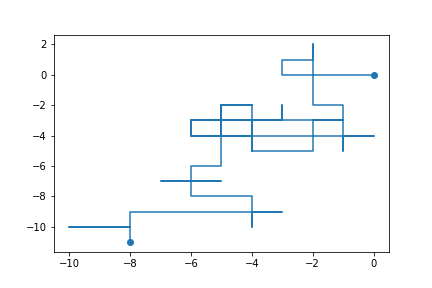
\includegraphics[width=\textwidth]{Rand_Path.png}
    \caption{}
    \label{fig:path_1}
\end{subfigure}
\hfill
\begin{subfigure}{0.5\textwidth}
    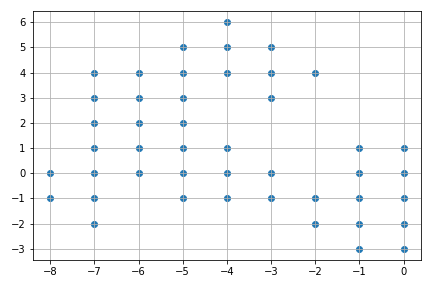
\includegraphics[width=\textwidth]{Rand_Path_Unique.png}
    \caption{}
    \label{fig:path_2}
\end{subfigure}
\vfill
\centering
\begin{subfigure}{0.5\textwidth}
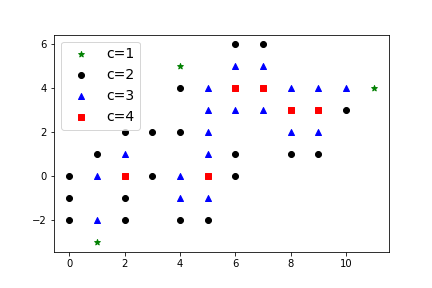
\includegraphics[width=\textwidth]{Rand_Path_Neigh.png}
\caption{}
\label{fig:path_3}
\end{subfigure}
\caption{
а) Сгенерированное блуждание модели RW $\{\omega_i\}$ \eqref{eq:DS_alg} из $N$ шагов. Концы блуждания отмечены жирными точками, ходы блуждания -- линией. 
Началом блуждания является зелёная точка $(0,0)$, концом блуждания -- черная, в которой так же рассчитывается атмосфера блужания $k$. 
б) Набор уникальных точек $\{\omega^u_i\}$ \eqref{eq:w_u}, принадлежащих блужданию модели RW, количество которых -- $\Nun$. 
в) Подсчёт соседей у каждого узла блуждания - доля узлов с k соседями считается по формуле \eqref{eq:n_i}.
}
\label{fig:path_alg}
\end{figure}

\section{Содержательная часть}

\subsection{Алгоритм генерации блужданий}

Блуждания $\{ \omega_ i \}$ генерируются в виде последовательности индексов направлений $ \{d_{i}\} $ в любой решётке, что ускоряет процесс моделирования. 
Первая точка блуждания на решётке $\omega_{0}$ лежит в начале координат $(0,0)$, далее блуждание определяется как последовательность узлов по формуле \eqref{eq:DS_alg}:
\begin{equation}
\{ \omega_i \} = 
\begin{cases}
\omega_{0} = (0,0) \\
\omega_{i} = \omega_{i-1} +\textup{steps}\left[d_{i}\right] 
\end{cases}
\begin{array}{l}
\textup{steps} = \left[(0,1), (0,-1), (1,0), (-1,0)\right], \\
d_i = \textup{Random}(\{0,1,2,3\}), i = 1..N,
\end{array}
\label{eq:DS_alg}
\end{equation}
где steps - массив фиксированных смещений из точки, определяемые законами решётки. 
Точность подсчёта наблюдаемых определяется лишь количеством повторов эксперимента.

С другой стороны, отсутствие требования непересекаемости блуждания вызывает ряд осложнений для сравнения результатов с классом блужданий без самопересечений. 
Например, возможны случаи, когда два идущих подряд направления противоположны друг другу - то есть, на i-м шаге блуждание смещается из точки $\omega_{i-1}$, а i+1-м - возвращается в него, то есть $\omega_{i-1} = \omega_{i+1}$.
В таком случае на графике блуждания возможны ''шипы'', концы которых будут узлами с всего одним соседом - основанием ''шипа''. 



Алгоритм обработки каждого модерируемого блуждания описан на картинках \ref{fig:path_1}, \ref{fig:path_2} и \ref{fig:path_3}:
\begin{itemize}
    \item Из сгенерированного блуждания (рисунок \ref{fig:path_1}) отбираются все уникальные точки узлов \eqref{eq:w_u} - образуется набор точек решётки $\{\omega^u_i\}, i = \{0, \Nun-1\}$ (рисунок \ref{fig:path_2}). Так же считается доля уникальных узлов блуждания \eqref{eq:nun}.
	\begin{equation}
	\begin{array}{l}
	\{ \omega^u_i \} = \textup{Unique}( \{ \omega_i \} ) \\
	N_{\textup{unique}} = |\{ \omega^u_i \}|
	\end{array}
	\label{eq:w_u}
	\end{equation}
    \item Для каждого уникального узла рассчитывается кол-во его соседей $c_i \in \{1,2,3,4\}$  (рисунок \ref{fig:path_3}).
    \item Доля узлов с k соседями считается как отношение количества уникальных узлов с k соседями к общему количеству уникальных узлов.
	\begin{equation}
	n_k = \frac{\sum_{i=0}^{\Nun-1}[c_i = k]}{\Nun}
	\label{eq:n_i}
	\end{equation}
\end{itemize}

\subsection{Результаты симуляций}

Была проведена генерация модели RW с количеством шагов $N = 10^{2}-10^{4}$. 
Доли уникальных узлов $\nun$ так же брались во внимание при симуляциях. 
Результаты симуляций, а так же количество итераций для каждой длины, описаны в таблице \ref{tab:Ran_Walk_neigh} и изображены на графиках \ref{fig:DS_n_i}, \ref{fig:DS_n_iu} и \ref{fig:DS_n_u}.

В следующих подразделах будет проведён анализ полученных результатов - сначала будет проведено обсуждение погрешностей данных, затем - оценка и сравнение шкалирующих функций \eqref{eq:f_i}, \eqref{eq:g_i} для наблюдаемых величин.

\begin{table}[h]
    \centering

\begin{tabular}{|c|c|c|c|c|c|c|}
\hline
N & M & $ \nun $ & $n_{1}$ & $n_{2}$ & $n_{3}$ & $n_{4}$ \\ \hline
100 & 96430000 & 0.490868(8) & 0.067676(3) & 0.33516(1) & 0.357310(7) & 0.239851(9) \\ \hline
150 & 69360000 & 0.462622(9) & 0.057825(3) & 0.30787(1) & 0.356280(7) & 0.27802(1) \\ \hline
200 & 36140000 & 0.44436(1) & 0.052236(4) & 0.29043(1) & 0.353706(9) & 0.30362(2) \\ \hline
350 & 17070000 & 0.41251(2) & 0.043761(4) & 0.26070(1) & 0.34590(1) & 0.34963(2) \\ \hline
500 & 7720000 & 0.39439(2) & 0.039590(5) & 0.24424(2) & 0.33965(2) & 0.37652(3) \\ \hline
750 & 4810000 & 0.37559(2) & 0.035672(5) & 0.22759(2) & 0.33188(2) & 0.40487(4) \\ \hline 
1000 & 2480000 & 0.36325(3) & 0.033333(6) & 0.21696(3) & 0.32610(2) & 0.42361(5) \\ \hline
3000 & 420000 & 0.32265(6) & 0.02650(1) & 0.18336(5) & 0.30351(5) & 0.4865(1) \\ \hline
5000 & 140000 & 0.30679(9) & 0.02434(1) & 0.17086(8) & 0.29322(8) & 0.5116(2) \\ \hline
6500 & 100000 & 0.2992(1) & 0.02330(2) & 0.16518(9) & 0.28816(9) & 0.5234(2) \\ \hline
7000 & 305000 & 0.29610(6) & 0.02302(1) & 0.16340(5) & 0.28657(5) & 0.5270(1) \\ \hline
8000 & 240000 & 0.29338(6) & 0.02253(1) & 0.16070(5) & 0.28409(6) & 0.5327(1) \\ \hline
9000 & 195000 & 0.29022(7) & 0.02215(1) & 0.15830(6) & 0.28185(6) & 0.5377(1) \\ \hline
10000 & 160000 & 0.28751(8) & 0.02179(1) & 0.15628(6) & 0.27991(7) & 0.5420(1) \\ \hline
\end{tabular}

    \caption{Средние доли узлов c 1-4-мя (столбцы $n_1$-$n_4$) соседями, а так же доля уникальных узлов (столбец $\nun$) в конформациях модели Random-Walk длин $10^{2}$-$10^{4}$ (столбец $N$). Также изображены на графиках \ref{fig:DS_n_i}, \ref{fig:DS_n_iu} и \ref{fig:DS_n_u}. В столбце $M$ выписано количество итераций алгоритма Монте-Карло.}
    \label{tab:Ran_Walk_neigh}
\end{table}

\begin{figure}[h]

\begin{subfigure}{0.5\textwidth}
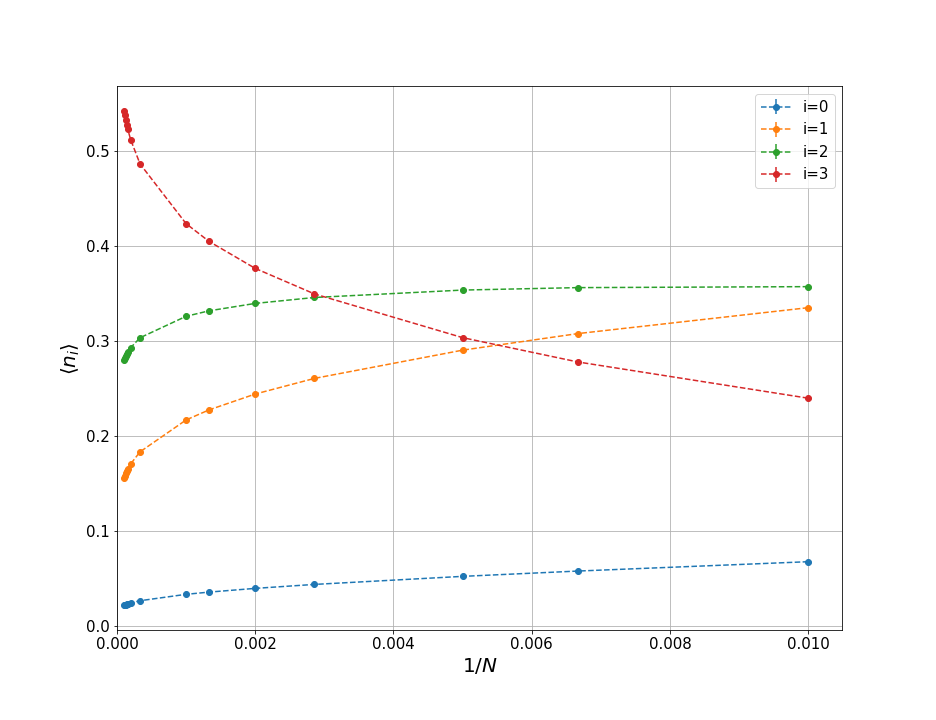
\includegraphics[width=\textwidth]{Rand_Path_n_i.png}
\caption{}
\label{fig:DS_n_i}
\end{subfigure}
\hfill
\begin{subfigure}{0.5\textwidth}
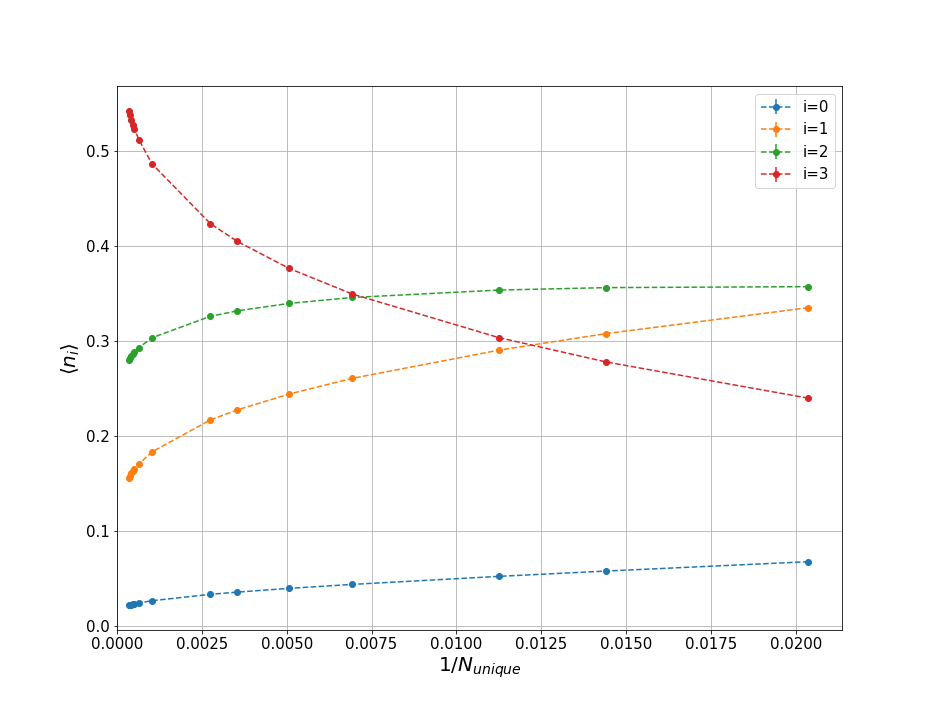
\includegraphics[width=\textwidth]{Rand_Path_n_i_unique.png}
\caption{}
\label{fig:DS_n_iu}
\end{subfigure}
\vfill
\centering
\begin{subfigure}{0.5\textwidth}
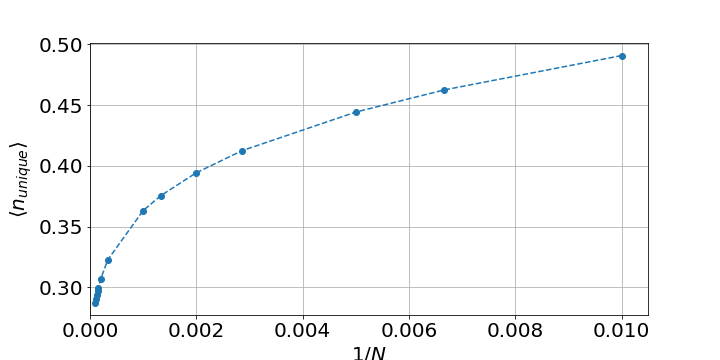
\includegraphics[width=\textwidth]{Rand_Path_n_unique.png}
\caption{}
\label{fig:DS_n_u}
\end{subfigure}
\caption{Доли узлов с фиксированным числом соседей (столбцы $n_1$-$n_4$ из таблицы \ref{tab:Ran_Walk_neigh}): а) от обратного количества шагов блуждания $1/N$; b) обратного количества уникальных узлов $1/\Nun$; c) Доли уникальных узлов (столбец $\nun$ из таблицы \ref{tab:Ran_Walk_neigh}) от обратного количества шагов блуждания $1/N$. }
\end{figure} 

\newpage

\subsection{Погрешности результатов}

Полученные в данной подсекции результаты имели ранее необоснованно большие погрешности, что потребовало более тщательного исследования. 
Необходимо проверить распределение результатов со временем, а так же сходимость средних наблюдаёмых величин и их ошибок.
 В качестве примера рассмотрим первую исследуемую длину $N=100$, т.к. именно её симуляции протекают быстрее всех.  

Распределение наблюдаемых долей узлов с фиксированным числом соседей 1-4, а так же доли уникальных узлов рассмотрены на гистограммах на левом графике рисунка \ref{fig:DS_100_dists_history}  в двух моментах времени: после $10^6$ шагов и после $2.5 \cdot 10^6$  шагов. 
На рисунке видно, что данные всех величин имеют нормальное или близко к нормальному распределению, а несимметричные склоны  некоторых величин ($n_1$ и $n_2$) объясняются близостью соответствующего края к нулю.

Сходимость наблюдаемых величин можно увидеть на правом графике \ref{fig:DS_100_dists_history}, где замеры средних проводились через каждые 4000 шагов. На графике средних заметна сходимость средней величины и уменьшение колебаний. 
С другой стороны, график среднего квадратического отклонения не стремится к нулю как ожидалось, а так же сходится с уменьшением колебаний к ненулевому значению. 
Это показывает противоречивость результатов (по крайней мере замеров ошибки - среднее явно сходится), причину чему следует искать в коде. 

Для удостоверения, что причина не лежит в jit-компиляции, был проведён запуск нескомпилированного с помощью numba кода. Результаты оказались идендичны с jit-компиляцией, и следовательно проблема в другом месте.

\begin{figure}
	\caption{Слева: Распределение долей узлов с 1-4 соседями и уникальных узлов блуждания длины 100 в два момента времени. Справа: История результатов (Столбец mean - средняя величина, столбец std - значение ошибки на i-м замере) долей узлов с 1-4 соседями и уникальных узлов блуждания длины 100 с интервалом замеров в 4000 шагов.}
     \label{fig:DS_100_dists_history}
\begin{minipage}{0.32\textwidth}
     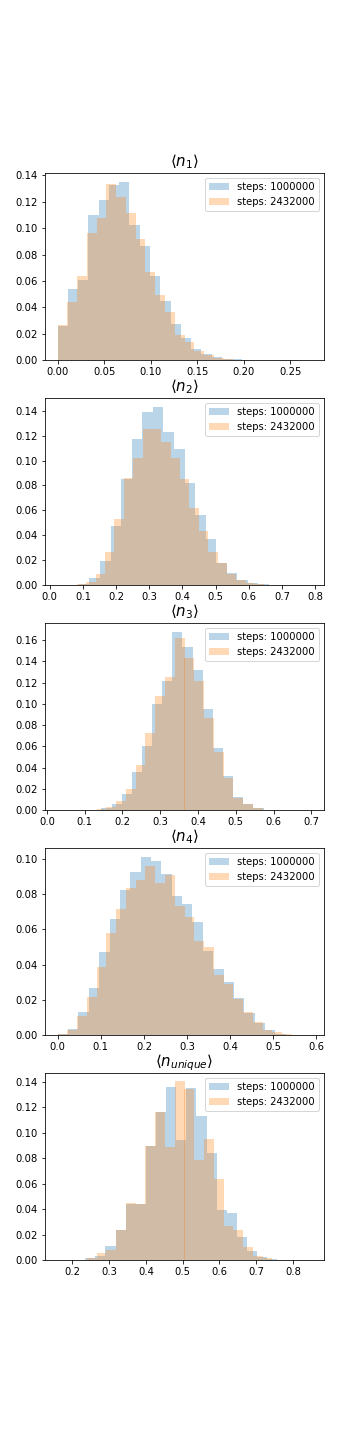
\includegraphics[width=\textwidth]{DS_100_dists.png}
\end{minipage}
\begin{minipage}{0.67\textwidth}
     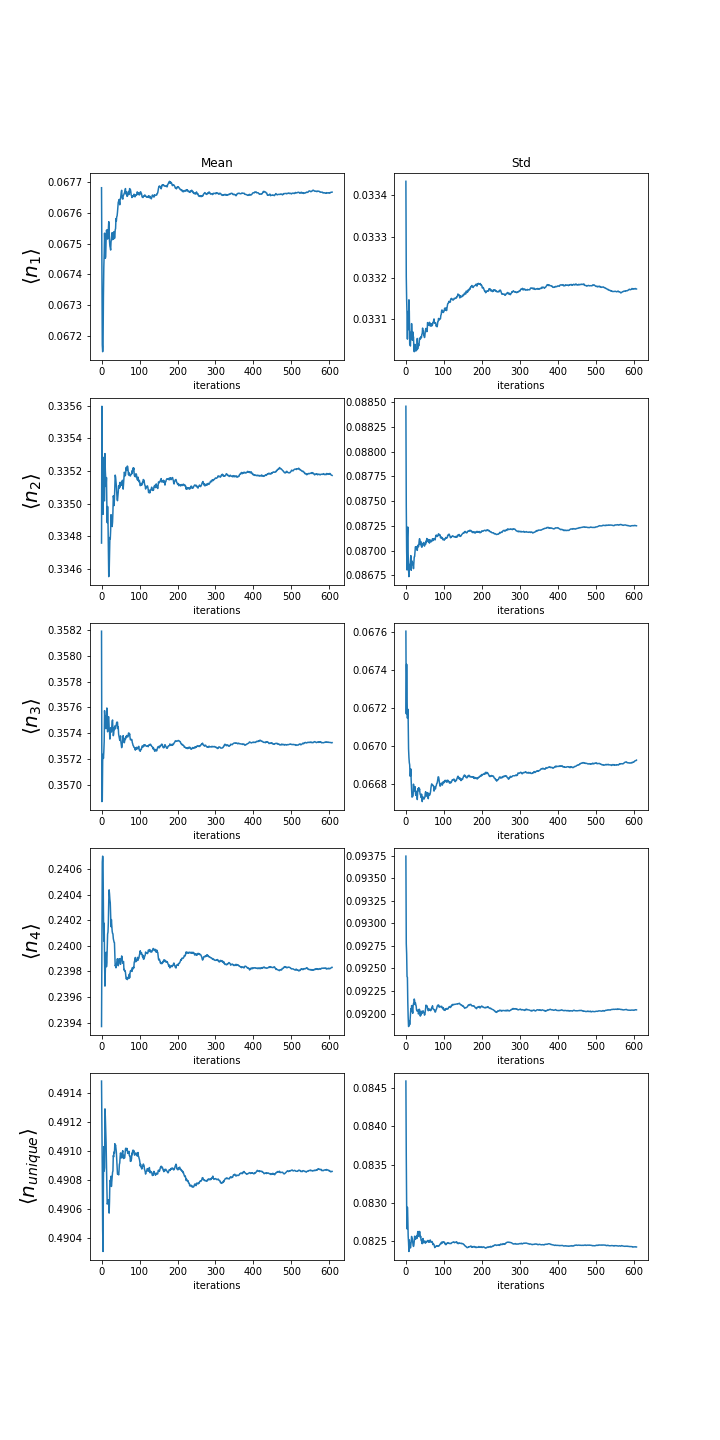
\includegraphics[width=\textwidth]{DS_100_history.png}
\end{minipage}
	
\end{figure}


Причиной столь больших погрешностей результатов была неверная интерпретация понятия "ошибка среднего", толковавшаяся ранее, как выборочное среднее квадратическое отклонение $\sigma(x)$ результатов симуляций $x$ - на деле ошибкой среднего является формула вида:

\[\Delta\la x \ra = \sigma(x)/\sqrt{N},\]

где  $N$ - объём выборки или количество экспериментов.


\subsection{Шкалирование результатов} \label{sec:ni_scale}

Применим к результатам из таблицы \ref{tab:Ran_Walk_neigh} те же методы анализа, что и ранее для доли узлов с фиксированным числом соседей в СБС -- определим характер шкалирования долей при стремлении длины конформации модели RW к бесконечности.
Рассмотрим данные в трёх предполагаемых масштабах: в линейной, лог-линейной и лог-логарифмической масштабностях от обратной длины $1/N$ и кол-ва уникальных узлов $1/\Nun$.
Пример исследуемых данных показан на графике \ref{fig:n1_scale}. 
На нём видно, что в случае лог-лог-шкалирования (или степенного) график обретает наилучшую среди трёх масштабностей линейность.
Оно же оказолось наиболее подходящим в графиках всех долей узлов $n_{1-4}$ в обоих функциях $f_i(N), g_i(\Nun)$, а так же для зависимости $\nun$ от кол-ва шагов $N$.

\begin{figure}
\centering
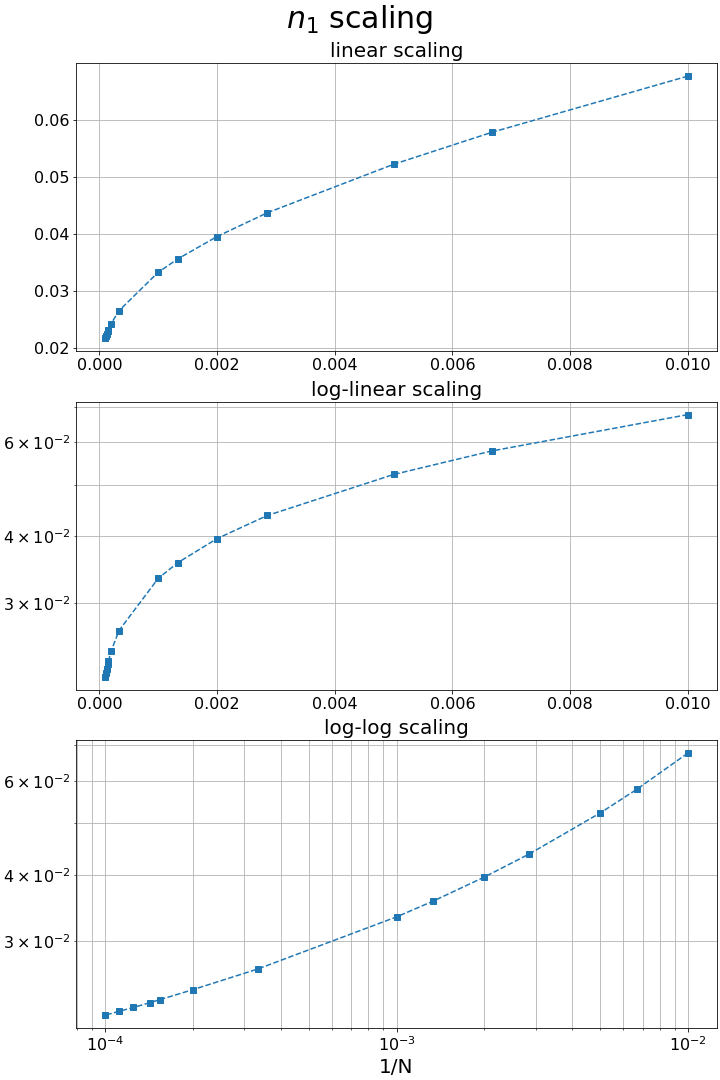
\includegraphics[width=0.7\textwidth]{n1_res.png}
\caption{Зависимость $n_1$ от $1/N$  в линейной, лог-линейной и лог-логарифмической масштабностях (сверху-вниз), по данным из таблицы \ref{tab:Ran_Walk_neigh}.} 
\label{fig:n1_scale}
\end{figure}

Тогда, шкалирующая функция $f_i(N)$ рассматривается в виде:

\begin{equation}
f_i(N) = k_i (1/N)^{a_i} + b_i,\ \ \ i \in \{1,2,3,4, \textup{unique}\}
\label{eq:n_i_log_log}
\end{equation}

Полученные коэффициенты с погрешностями выписаны на таблице \ref{tab:n_i_log_log}.

\begin{table}[h]
\centering
\begin{tabular}{|c|c|c|c|c|}
\hline
 & k & a & b & N \\ \hline
$n_1$ & 0.3425(8) & 0.417(2) & 0.014(1) & 3000-10000 \\ \hline
$n_2$ & 0.573(4) & 0.171(1) & 0.037(2) & 3000-10000 \\ \hline
$n_3$ & 0.588(3) & 0.219(3) & 0.202(3) & 3000-10000 \\ \hline
$n_4$ & -1.239(9) & 0.189(3) & 0.759(5) & 500-10000 \\ \hline
$n_{unique}$ & 0.831(1) & 0.2049(2) & 0.1616(4) & 500-10000 \\ \hline
\end{tabular}
\caption{Коэффициенты степенной шкалирующей функции доли узлов от обратного количества шагов блуждания $1/N$ \eqref{eq:n_i_log_log}.}
\label{tab:n_i_log_log}
\end{table}
Аналогичный анализ проведён для зависимости долей узлов $n_1 - n_4$ от количества уникальных узлов $\Nun$:

\begin{equation}
g_i (\Nun) = q_i  (1/\Nun)^{s_i} + d_i,\ \ \ i \in \{1,2,3,4\}
\label{eq:n_i_u_log_log}
\end{equation}

\begin{table}[h]
\centering
\begin{tabular}{|c|c|c|c|c|}
\hline
 & q & s & d & $\Nun$ \\ \hline
$n_1$ & 0.313(1) & 0.479(2) & 0.015(1) & 967-2875 \\ \hline
$n_2$ & 0.567(3) & 0.214(1) & 0.053(2) & 967-2875 \\ \hline
$n_3$  & 0.542(5) & 0.244(2) & 0.203(2) & 967-2875 \\ \hline
$n_4$ & -1.20(1) & 0.225(4) & 0.741(5) & 197-2875 \\ \hline
\end{tabular} 
\caption{Коэффициенты степенной шкалирующей функции доли узлов от обратного количества уникальных узлов блуждания $1/\Nun$ \eqref{eq:n_i_u_log_log}.}
\label{tab:n_i_u_log_log}
\end{table}

\newpage 

\subsection{Зависимость доли уникальных узлов от количества шагов}

В данном подразделе проверяется численная эквивалентность фитирующих функций долей узлов $n_1-n_4$: $f_i$ \eqref{eq:n_i_log_log}, имееющей прямую зависимость от числа шагов $N$ и $g_i(\Nun)$ \eqref{eq:n_i_u_log_log}, со сложной зависимостью от $N$.

\begin{equation}
	\la n_i \ra = g_i(\Nun) = q_i (1/\Nun)^{s_i} + d_i
	\label{eq:gi_approx1}
\end{equation}

Из результатов прошлого подраздела были получены коэффициенты фитирующей функции $\nun$ (строка $\nun$ таблицы \ref{tab:n_i_log_log}). Определим их как $k_u, a_u, b_u$ соответственно и раскроем их в функции аргумента: 

\begin{equation}
	\Nun = N \nun(N) = N (k_u (1/N)^{a_u} + b_u)
	\label{eq:gi_appprox2}
\end{equation}

Рассмотрим аппроксимацию произвольной функции $g_i(\Nun)$ с выражением её аргумента через $N$.
Подставим \eqref{eq:gi_appprox2} в \eqref{eq:gi_approx1} и проведём линеаризацию - сначала $1/\Nun(N)$ при $1/N \to 0$, а затем $(1/\Nun(N))^{s_i}$ при $1/N \to 0$:

\begin{Large}
\begin{equation*}
\begin{array}{l}
1)\ \ \ \ \ (N (b_u + k_u(1/N)^{a_i})^{-1} = ( N b_u)^{-1} (1 + \frac{k_u}{b_u} \frac{1}{N^{a_u}})^{-1} = \frac{1}{b_u N} (1 - \frac{k_u}{b_u} \frac{1}{N^{a_u}} + O(\frac{1}{N^{2a_u}})) \\
\\
2)\ \ \ \ \ ( - // - )^{s_i}  = \frac{1}{(b_u N)^{s_i}} \ \  (1 - \frac{k_u}{b_u} \frac{1}{N^{a_u}} + O(\frac{1}{N^{2a_u}}))^{s_i} = \frac{1}{(b_u N)^{s_i}}\ \ (1 - \frac{k_u s_i}{b_u} \frac{1}{N^{a_u}} + O(\frac{1}{N^{2a_u}}))
\end{array}
\end{equation*}
\end{Large}

Итоговое выражение примет следующий вид:

\begin{large}
\begin{equation}
g_i(N) = \frac{k_i}{b_u^{s_i}} \frac{1}{N^{s_i}} - \frac{k_i s_i k_u}{b_u^{a_i+1}} \frac{1}{N^{a_u+s_i}} + d_i + O(\frac{1}{N^{2 a_u +s_i}}),\ \ \ \ \ N \to \infty
\end{equation}
\label{eq:g_n_expect}
\end{large}

Таким образом, мы свели функцию $g_i(\Nun)$ \eqref{eq:gi_approx1} к функции вида \eqref{eq:n_i_log_log}, сохранив дополнительные степенные поправки. 
Очевидно, линеризация повлияет на поведение в функции области небольших длин блуждания, поэтому оценивать теорически ожидаемые линейный и степенной коэффициент по полученной функции \eqref{eq:g_n_expect} невозможно.
Это объясняет различие коэффициетов $k_i, s_i$. 

С другой стороны, проведенные преобразования не дали никакой поправки для асимптотического предела $d_i$ - следовательно, вне зависимости от взятого аргумента, $N$ или $\Nun$, функции соответствующих долей узлов с фиксированным числом соседей $f_i$ и $g_i$ должны сходиться на бесконечности в одной точке, а столбцы $b$ и $d$ таблиц \ref{tab:n_i_log_log} \ref{tab:n_i_u_log_log} соответственно - равными в пределах погрешностей.
Это так же подтверждается тем, что если $N \to \infty$, то и, очевидно $\Nun \to \infty$, поскольку $b_u > 0$.  

Рассмотрим графики трёх функций на каждую долю $n_1$-$n_4$: как функцию $f_i(N)$, как функцию $g_i(N\nun(N))$, а так же аппроксимацию второй функции \eqref{eq:g_n_expect}.

Графики функций в линейном масштабе изображены на рисунке \ref{fig:ni_fn_vs_gNun}. По ним видно, что функция $f(N)$ и $g(\Nun(N))$ почти не имеют отличий, что говорит о полном взаимозаменяемости аргументов и правильности полученных результатов на небольших длинах. Зелёная линия соответствует аппроксимирующему виду $g(\Nun(N))$ и имеет поправку, уменьшающуюся при стремлении $N$ к бесконечности, но так же визуально сливается с первыми двумя функциями в области больших $N$.

\begin{figure}
\centering
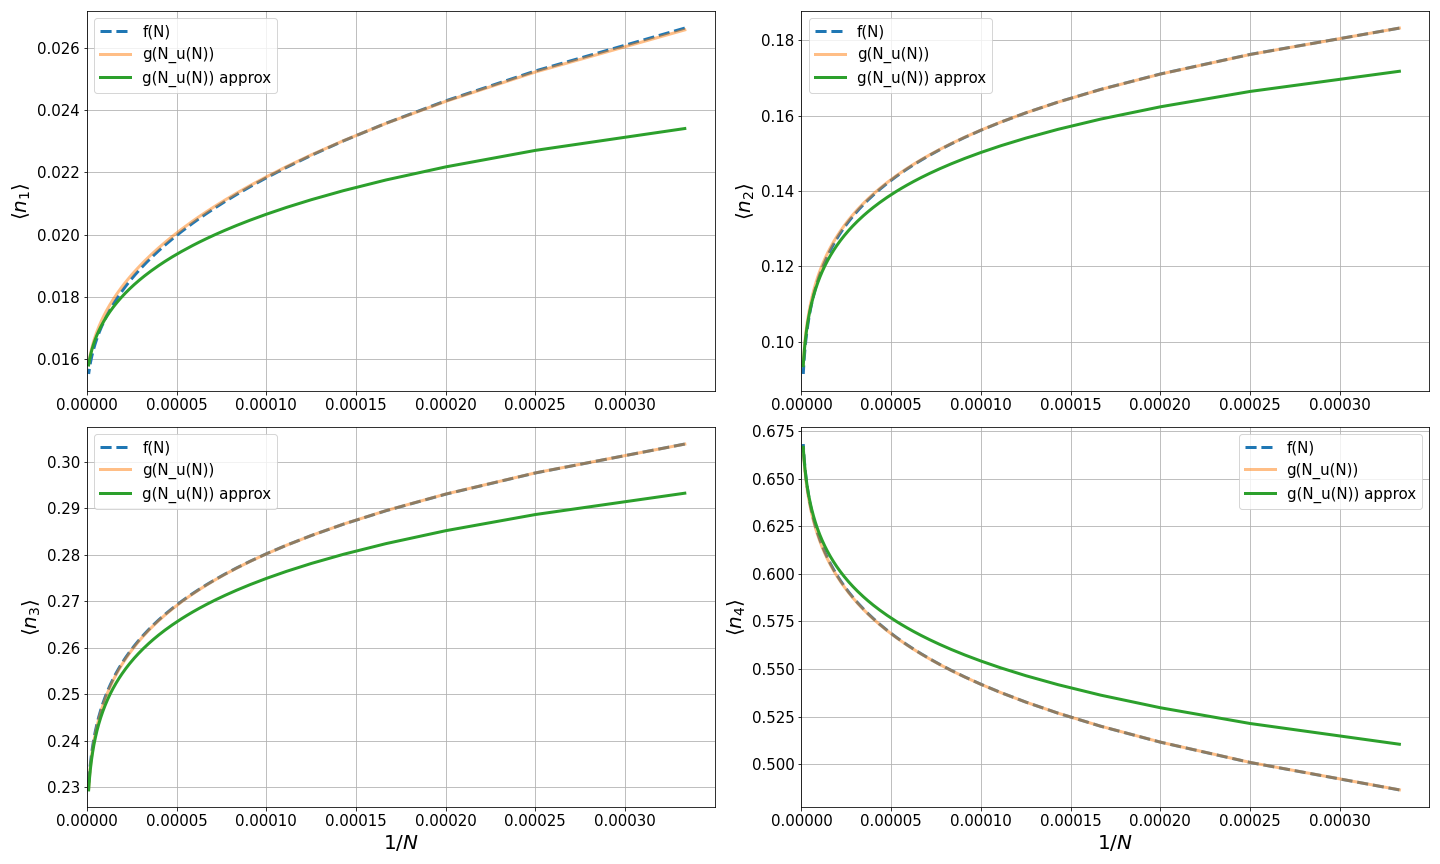
\includegraphics[width=\textwidth]{n_i_fN_vs_gNun.png}
\caption{Доли узлов $n_1-n_4$ в линейном масштабе как функции от количества шагов (синий пунктир) \eqref{eq:n_i_log_log}, а так же сложные функции от количества уникальных узлов от количества шагов (оранжевая линия -- прямая подстановка функций  \eqref{eq:gi_appprox2} в \eqref{eq:gi_approx1}, зелёная - аппроксимация \eqref{eq:g_n_expect}), по горизонтали -- обратное количество шагов блуждания $1/N$. Коэффициенты взяты из таблиц \ref{tab:n_i_log_log} и \ref{tab:n_i_u_log_log}.}
\label{fig:ni_fn_vs_gNun}
\end{figure}

Логарифмический масштаб графиков представлен на рисунке \ref{fig:ni_fn_vs_gNun_log}. 
Здесь ситуация выглядит совершенно иначе: на всех графиках наблюдается расхождение $f_i$ и $g_i$ по мере сближения с нулём.
Причём теперь $g_i$ и её аппроксимация сливаются в одну кривую (что говорит о правильности полученной линеризацией функции \eqref{eq:g_n_expect}). 
Из прошлого раздела мы узнали, что асимпотические пределы $n_1$ и $n_3$ равны в пределах погрешности между выбранными зависимостями.

Однако пределы двух других функций как численно, так и графически расходятся между $f_i$ и $g_i$, что противоречит предположениям о связи зависимостей в пределе бесконечного числа шагов блуждания.


\begin{figure}
\centering
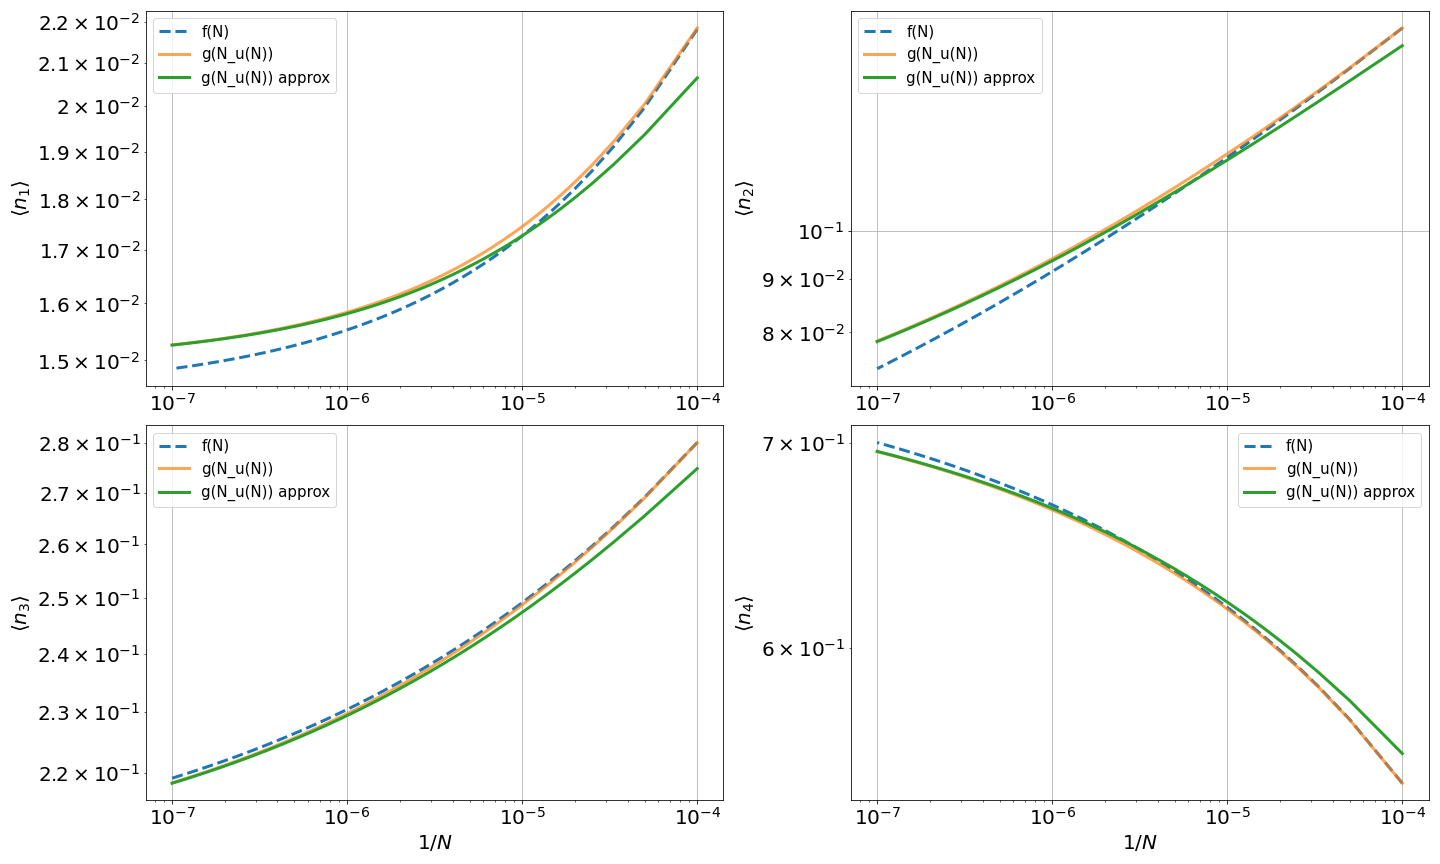
\includegraphics[width=\textwidth]{n_i_fN_vs_gNun_log.png}
\caption{Доли узлов $n_1$-$n_4$ в лог-лог масштабе как функции от количества шагов (синий пунктир) \eqref{eq:n_i_log_log}, а так же сложные функции от количества уникальных узлов от количества шагов (оранжевая линия -- прямая подстановка функций  \eqref{eq:gi_appprox2} в \eqref{eq:gi_approx1}, зелёная - аппроксимация \eqref{eq:g_n_expect}), по горизонтали -- обратное количество шагов блуждания $1/N$. Коэффициенты взяты из таблиц \ref{tab:n_i_log_log} и \ref{tab:n_i_u_log_log}.}
\label{fig:ni_fn_vs_gNun_log}
\end{figure}
\subsection{Итоговое сравнение функций долей узлов $n_i$}
\label{sec:n_final}

Данный подраздел завершает сравнение функций $f_i$ \eqref{eq:n_i_log_log} и $g_i$ \eqref{eq:n_i_u_log_log}, на этот раз напрямую оценивая их сходство по линейным, степенным и свободным коэффициентам соответственно.

В первую очередь сравним свободные коэффициенты шкалирующих функций \eqref{eq:n_i_log_log}, \eqref{eq:n_i_u_log_log} (cтолбцы $b$ и $d$ таблиц \ref{tab:n_i_log_log} и \ref{tab:n_i_u_log_log} соответственно) построчно. Очевидно, несмотря на разные структуры функций ($f_i$ - функция от $N$, $g_i$ - фактически сложная функция от $N$), пределы функций $f_1$ и $g_1$, $f_2$ и $g_2$ и т.д. должны полностью совпадать, так как $\Nun \to \infty$ при $N \to \infty$. Так же, в виду обнаруженного степенного характера шкалирования величин при бесконечном количестве шагов, интересно различие между ближайшими к пределу результатами симуляций Монте-Карло (последняя строка таблицы \ref{tab:Ran_Walk_neigh}) и полученными пределами. 

\begin{table}[h]
\centering
\begin{tabular}{|c|c|c|c|}
\hline
 & b & d & $n_i(N=10000)$ \\ \hline
$n_1$ & 0.014(1) & 0.015(1) & 0.02179(1)\\ \hline
$n_2$ & 0.037(2) & 0.053(2) & 0.15628(6)\\ \hline
$n_3$ & 0.202(3) & 0.203(2) & 0.27991(7)\\ \hline
$n_4$ & 0.759(5) & 0.741(5) & 0.5420(1)\\ \hline
\end{tabular}
\caption{Пределы шкалирующих функций долей узлов (с фиксированным числом соседей, построчно) от $N$ \eqref{eq:n_i_log_log} (левый столбец), от $\Nun$ \eqref{eq:n_i_u_log_log} (центральный столбец) и ближайшие к пределу результаты Монте-Карло (правый столбец).}
\label{tab:bd_compare}
\end{table}

Наглядное сравнение проведено на таблице \ref{tab:bd_compare}. 
Видно, что лишь у двух величин из четырех свободные коэффициенты шкалирующих функций равны между собой в пределах погрешности - это пределы долей $n_1$ ($b_1$ и $d_1$) и $n_3$ ($b_3$ и $d_3$). 
Другие два предела значительно отличаются -- их разница многократно превышает погрешность.
Однако между функциями сохраняется соразмерность пределов: как $b_1 < b_2 < b_3 < b_4$, так и $d_1 < d_2 < d_3 < d_4$.


Так же особо примечательна огромная разница между результатами симуляций Монте-Карло и соответствующими пределами у всех величин.
Это показывает значительное влияние степенной составлящей функций вблизи $1/N \to 0$.

\begin{table}[h]
\centering
\begin{tabular}{|c|c|c|}
\hline
 & a & s \\ \hline
$n_1$ & 0.417(2) & 0.479(2) \\ \hline
$n_2$ & 0.171(1) & 0.214(1) \\ \hline
$n_3$ & 0.219(3) & 0.244(2) \\ \hline
$n_4$ & 0.189(3) & 0.225(4) \\ \hline
\end{tabular}
\caption{Степенные коэффициенты шкалирующих функций долей узлов (с фиксированным числом соседей, построчно) от $N$ \eqref{eq:n_i_log_log} (левый столбец) и от $\Nun$ \eqref{eq:n_i_u_log_log} (правый столбец).}
\label{tab:as_compare}
\end{table}

Проведём аналогичное сравнение степенных коэффициентов $a$ и $s$ шкалирующих функций \eqref{eq:n_i_log_log}, \eqref{eq:n_i_u_log_log} относительно соответствующей наблюдаемой величины на таблице \ref{tab:as_compare}. 
Численная схожесть степенных коэффициентов функций не наблюдается ни при каких величинах $n_i$.
Заметно, что коэффициенты функций $g_i$ несколько больше чем у функций $f_i$.
Из этого можно справедливо предположить, что число уникальных узлов $\Nun$ обладает более сильными геометрическими свойствами, чем количество шагов $N$. 
Это так же подтверждается результатами шкалирования доли уникальных узлов (строка $\nun$ таблицы \ref{tab:n_i_log_log}) -- доля уникальных узлов случайного бесконечно долгого блуждания очень небольшая, чуть больше $16\%$.
Выходит, в бесконечно отдалённый момент времени блужданию нужно совершить в среднем больше 6 шагов, чтобы найти не посещённый ранее узел решётки.

Сохраняется соразмерность степенных коэффициентов: как $a_1 > a_3 > a_4 > a_2$, так и $s_1 > s_3 > s_4 > s_2$. 
Примечательно так же то, что у величин с наименьшими степенными коэффициентами среди всех четырех ($n_2, n_4$) имеют разные пределы функций $f_i$ и $g_i$ - можно предположить, что это вызвано техническими особенностями метода наименьших квадратов, использованного для оценки коэффициентов шкалирующих функций.
Малое значение степеного коэффициента шкалирующей функции означает слабое движение антиградиента функции ошибок.
Это даёт понимание, что фактически погрешность пределов функций $f_i$ и $g_i$ больше, чем была подсчитана методом ранее. 


\begin{table}[h]
\centering
\begin{tabular}{|c|c|c|}
\hline
 & k & q \\ \hline
$n_1$ & 0.3425(8) &  0.313(1) \\ \hline
$n_2$ & 0.573(4) & 0.567(3) \\ \hline
$n_3$ & 0.588(3) & 0.542(5) \\ \hline
$n_4$ & -1.239(9) & -1.20(1) \\ \hline
\end{tabular}
\caption{Линейные коэффициенты шкалирующих функций долей узлов (с фиксированным числом соседей, построчно) от $N$ \eqref{eq:n_i_log_log} (левый столбец) и от $\Nun$ \eqref{eq:n_i_u_log_log} (правый столбец).}
\label{tab:kq_compare}
\end{table}

Сравнение линейных коэффициетов изображено на таблице \ref{tab:kq_compare}. 
В данном случае между функциями не наблюдается ни численного, ни соразмерного сходства - несмотря на равенство всех коэффициентов до первого знака после запятой, в пределах погрешности равенства нет.

Имеется лишь знаковое сходство -- все коэффициенты функций, кроме $k_4$ и $q_4$, положительны, что говорит о сохранении схожести функций по поведению.

В итоге, с некоторым допущением относительно используемых методов апроксимации, мы получили примерное равенство пределов шкалирующих функций от $N$ и от $\Nun$, что говорит о корректности полученных функций шкалирования.


\newpage
\section{Исследование поведения концов блужданий модели RW}
\label{sec:atm}

Следующие разделы посвящены исследованию поведения частного случая локального координационного числа на конце блуждания, или ''атмосфере'' блуждания. 
В качестве основной наблюдаемой берётся $\pkn$ -- вероятность существования блуждания с количеством шагов $N$ с атмосферой $k$.
Атмосферу блуждания можно легко посчитать как разность координационного числа решётки (для квадратной - 4) и локального координационного числа (число соседей вокруг узла) на конце блуждания.
В рамках симуляций Монте-Карло данная наблюдаемая считается среди сгенерированной выборки:

\begin{large}

\begin{equation}
\begin{array}{l}
a_t = 4 - c_{\textup{end}}(t), \\
\pkn = \frac{\sum_{t=0}^{\textup{M}} [a_t = k]}{\textup{steps}},
\label{eq:pkn}
\end{array}
\end{equation}

\end{large}
где $c_{\textup{end}}(t)$ -- число соседей на конце t-го сгенерированного блуждания, $\textup{M}$ -- объём сгенерированной выборки, а $a_t$ -- атмосфера t-го сгенерированного блуждания. Пример подсчёта атмосферы блуждания изображен на рисунке \ref{fig:path_atm}.

Ранее исследование данного свойства проводилось в работе \cite{owczarek2008scaling}, на невзаимодействующих случайных блужданиях без самопересечений. 
Так же подобная задача рассматривалась в книге \cite{Spitser1969}, на странице 206 под номером 9, для \textit{возвратного простого случайного блуждания}. Задача формулируется следующим образом:

\begin{itemize}
    \item Случайное блуждание на квадратной решётке начинается из некоторой точки $x_0 = \chi$, не лежащей в начале координат.
    \item Процесс случайного блуждания длится не фиксированное количество шагов, а до фиксированной \textit{точки остановки} - до достижения блужданием начала коордиинат $x_{\textup{end}} = 0$
    \item До достижения точки остановки блуждание может посетить одну или несколько соседних с ним точек - (0,1), (1,0), (0,-1), (-1,0). Пусть число уникальных посещенных блужданием соседних точек  $N \in \{1, 2, 3, 4\}$
    \item Задачей является вычислить вероятности блуждания посетить каждое возможное количество уникальных соседних точек для бесконечно удаленной от начала координат начальной точки блуждания $\chi$:
    
    \[ p_{n} = \lim_{|\chi|\to \infty} P_{\chi}[N = n] =\ ?,\ \ \ n = 1, 2, 3, 4\]
\end{itemize}

Так же в качестве подсказки было указано, что отношение $p_1:p_2:p_3:p_4$ почти равно $4:3:2:1$.
Пример возвратного блуждания с точкой остановки в начале координат изображен на рисунке \ref{fig:path_spitser}. 

\begin{figure}[h]
    
\begin{subfigure}{0.5\textwidth}
    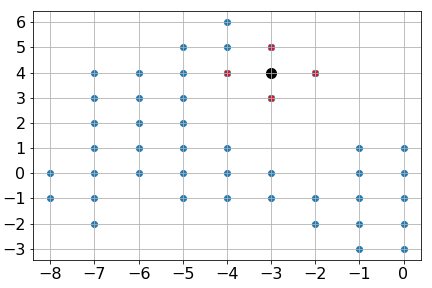
\includegraphics[width=\textwidth]{Rand_Path_Atm.png}
    \caption{}
    \label{fig:path_atm}
\end{subfigure}
\hfill
\begin{subfigure}{0.5\textwidth}
    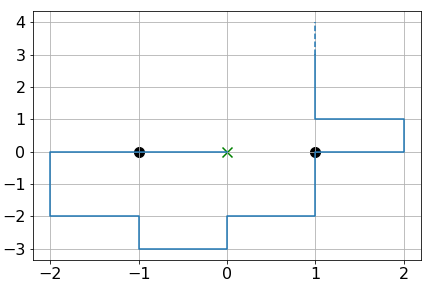
\includegraphics[width=\textwidth]{Spitser.png}
    \caption{}
    \label{fig:path_spitser}
\end{subfigure}
\caption{а) Подсчёт атмосферы блуждания модели RW (продолжение рисунков \ref{fig:path_alg}). Для данного блуждания все соседние узлы его конца уже посещены ранее, атмосфера блуждания $a=0$. b) Пример исследуемого блуждания в задаче \cite{Spitser1969}: из бесконечно удаленной точки (движение отмеченно пунктиром) блуждание посетило две соседние началу координат точки (отмечены чёрным), прежде чем остановилась в нём (точка остановки отмечена зелёным крестиком).}
\end{figure}



В рамках летней производственной практики (см. Отчёт о практике) задача из работы Спитцера была теоретически и экспериментально решена. 
Результаты расчётов можно увидеть в таблице \ref{tab:Spitser_res}:

\begin{table}[h]
	\centering
	\begin{tabular}{|c|c|c|c|c|}
	\hline
	$p_1$ &  $p_2$ & $p_3$ &  $p_4$ \\ \hline
 	0.393566 & 0.314680 & 0.190025 & 0.101729 \\ \hline
	\end{tabular}
	\caption{Аналитическое решение задачи из работы  \cite{Spitser1969}}
	\label{tab:Spitser_res}
\end{table}

В разделе \ref{sec:ni_scale} были найдены пределы долей узлов с фиксированным числом соседей $n_i$ \eqref{eq:n_i}.
Задачей следующих разделов, аналогично исследованию долей $n_i$, будет определение характера шкалирования $\pkn$ \eqref{eq:pkn}, оценка коэффициентов шкалирующих функций, а так же сравнение асимптотических пределов вероятностей $\pkn$ при стремлении числа шагов блуждания к бесконечности ($N \to \infty$):

\begin{enumerate}
\item с ответами на ранее описанную задачу \cite{Spitser1969}
\item с найденными в разделе \ref{sec:ni_scale} пределами долей $n_i$ \eqref{eq:n_i} (таблицы \ref{tab:n_i_log_log} и \ref{tab:n_i_u_log_log})
\end{enumerate}

\newpage

\subsection{Зависимость атмосфер от количества шагов блуждания и уникальных узлов}

Была рассчитана вероятность блуждания модели RW фиксированной длины $N$ иметь атмосферу $k$. 
Под длиной блуждания $N$ здесь имеется в виду количество случайных шагов, проделанных блужданием, без учёта, сколько уникальных узлов оно занимает.
Результаты можно увидеть в таблице \ref{tab:randw_p_atm} и на графиках \ref{fig:randw_p_atm}, как функции от $N$, и \ref{fig:randw_p_atm_u}, как функции от $\Nun$.

\begin{figure}[h]
    
\begin{subfigure}{0.49\textwidth}
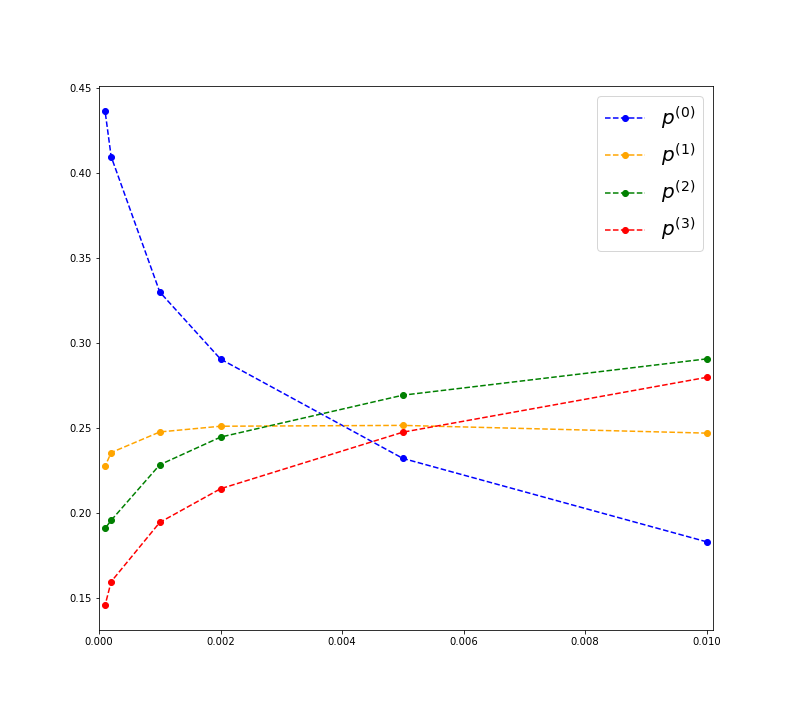
\includegraphics[width=\textwidth]{randwalk_p_atmos.png}
\caption{}
\label{fig:randw_p_atm}
\end{subfigure}
\hfill
\begin{subfigure}{0.49\textwidth}
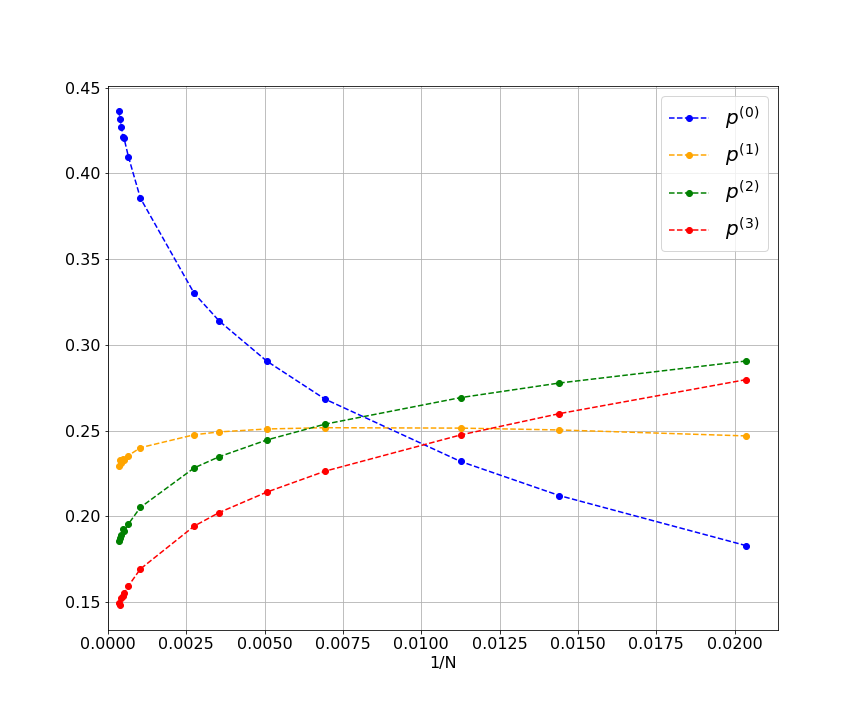
\includegraphics[width=\textwidth]{randwalk_p_atmos_unique.png}
\caption{}
\label{fig:randw_p_atm_u}
\end{subfigure}
\caption{Вероятность конформации модели RW  иметь атмосферу k=0,1,2,3  (столбцы $p^{(0)}$-$p^{(3)}$ из таблицы \ref{tab:randw_p_atm}): от a) от обратного количества шагов $1/N$ (столбец $N$); b) от обратного количества уникальных узлов $\Nun = N\nun$.}
\label{fig:randw_p_full}
\end{figure} 

\begin{table}[h] 
\centering
\begin{tabular}{|c|c|c|c|c|c|c|}
\hline
N & M & $ \nun $ & $p^{(0)}$ & $p^{(1)}$ & $p^{(2)}$ & $p^{(3)}$ \\ \hline
100 & 96430000 & 0.490868(8) & 0.182831 & 0.246855 & 0.290593 & 0.279720 \\ \hline
150 & 69360000 & 0.462622(9) & 0.212044 & 0.250342 &0.277737 &0.259877 \\ \hline
200 & 36140000 & 0.44436(1) & 0.231971 & 0.251413 & 0.269204 & 0.247413 \\ \hline
350 & 17070000 & 0.41251(2) & 0.268341 & 0.251656 &0.253724 & 0.226279 \\ \hline
500 & 7720000 & 0.39439(2) & 0.290471 & 0.250914 & 0.244515 & 0.214100 \\ \hline
750 & 4810000 & 0.37559(2) & 0.313906 & 0.249196 & 0.234730 & 0.202167 \\ \hline 
1000 & 2480000 & 0.36325(3) & 0.329962 & 0.247547 & 0.228218 & 0.194273 \\ \hline
3000 & 420000 & 0.32265(6) & 0.385626 & 0.239993& 0.205155 & 0.169226 \\ \hline
5000 & 140000 & 0.30679(9) & 0.409736 & 0.235407 & 0.195493 & 0.159364  \\ \hline
6500 & 100000 & 0.2992(1) & 0.420400 & 0.232740 & 0.191620 & 0.155240 \\ \hline
7000 & 305000 & 0.29610(6) & 0.421036 & 0.233311 & 0.192348 & 0.153305  \\ \hline
8000 & 240000 & 0.29338(6) & 0.427387 & 0.230854 & 0.189233 & 0.152525 \\ \hline
9000 & 195000 & 0.29022(7) & 0.431959 & 0.232795 & 0.187205 & 0.148041 \\ \hline
10000 & 160000 & 0.28751(8) & 0.436369 & 0.229075 & 0.185300 & 0.149256 \\ \hline
\end{tabular}
\caption{Результаты экспериментов, описанных на графиках \ref{fig:randw_p_atm} и \ref{fig:randw_p_atm_u}: столбцы $p^{(0)}$-$p^{(3)}$ показывают среднюю вероятность $\pkn$ \eqref{eq:pkn} блуждания модели RW с количеством шагов $N$ иметь атмосферу 0-3 соответственно, объём сгенерированной выборки блужданий для каждой длины записан в столбце $M$.}
\label{tab:randw_p_atm}
\end{table}

Первичное рассмотрение графиков зависимости вероятностей от обратной длины $1/N$ в линейной, лог-линейной и лог-логарифмической масштабностях показало, что график лучше всего выпрямляется в третьем случае. 
Аналогичный результат показали графики остальных вероятностей, как функций от $N$ так и от $\Nun$.
Поэтому для всех четырех вероятностей аппроксимирующая функция при $N \to \infty$ ищется так же, как и для долей узлов, в двух видах - сначала как функция от количества шагов блуждания $N$, по формуле \eqref{eq:pi_N}.

\begin{equation}
p^{(i)}(N) = k_i  (1/N)^{a_i} + b_i, \ \ \ i \in \{ 0,1,2,3\} \\
\label{eq:pi_N}
\end{equation}

где $k_i$ - линейный наклонный коэффициент, $a_i$ - степенной коэффициент, а $b_i$ - свободный коэффициент. 
Оно же является пределом вероятности $p^{(i)}$ при $N \to \infty$.
Для поиска коэффициентов использовался метод наименьших квадратов.
Результаты апроксимации графиков вблизи $1/N \to 0$, диапазон выбранных длин цепочек для подбора функции,
а так же стартовое положение описаны в таблицах \ref{tab:p_i_log_log} и \ref{tab:p_i_u_log_log}. 

\begin{table}[h] 
\centering
\begin{tabular}{|c|c|c|c|c|c|}
\hline
 & $k_i$ & $a_i$ & $b_i$ & N & start  \\ \hline
$p^{(0)}$ & -1.17(1) & 0.202(7) & 0.62(1) & 3000-10000 & -1, 1, 0.4 \\ \hline 
$p^{(1)}$ & 0.54(1) & 0.37(3) & 0.213(6) & 3000-10000 & 0.5, 0.5, 0.245 \\ \hline
$p^{(2)}$ & 0.596(4) & 0.272(6) & 0.137(4) & 1000-10000 & 0.5, 0.5, 0.16 \\ \hline
$p^{(3)}$ & 0.613(5) & 0.259(6) & 0.092(4) & 750-10000 & 0.5, 0.5, 0.15 \\ \hline
\end{tabular}
\caption{Коэффициенты степенных функций, аппроксимирующих вероятности $p^{(0)}$-$p^{(3)}$ от $1/N$ по формуле \eqref{eq:pi_N}, описанных на графиках \ref{fig:p_03_loglog}. Столбец start показывает начальное приближение коэффициентов в методе наименьших квадратов.}
\label{tab:p_i_log_log}
\end{table}

\begin{equation}
p^{(i)}(\Nun) = q_i  (1/\Nun)^{s_i} + d_i, \ \ \ i \in \{ 0,1,2,3\}
\label{eq:pi_Nu}
\end{equation}

\begin{table}[h]
\centering
\begin{tabular}{|c|c|c|c|c|c|} \hline
 & $q_i$ & $s_i$ & $d_i$ & $\Nun$ & start  \\ \hline
$p^{(0)}$ & -1.142(9) & 0.25(1) & 0.59(2) & 1533-2875 &  -1, 1, 0.7 \\ \hline
$p^{(1)}$ & 0.52(1) & 0.44(4) & 0.214(6) & 967-2875 & 0.5, 0.5, 0.23\\ \hline
$p^{(2)}$ & 0.585(5) & 0.323(7) & 0.141(3) & 363-2875  & 0.5, 0.5, 0.16\\ \hline
$p^{(3)}$ & 0.604(5) & 0.310(6) & 0.097(3) & 281-2875 & 0.5, 0.5, 0.15\\ \hline
\end{tabular}

\caption{Коэффициенты шкалирующих функций вероятности $p^{(0)}$-$p^{(3)}$ от $1/N_{unique}$ по формуле \eqref{eq:pi_Nu}. Столбец start показывает начальное приближение коэффициентов в методе наименьших квадратов.}
\label{tab:p_i_u_log_log}
\end{table}

Графики зависимости от $1/N$ представлены на рисунках \ref{fig:p_03_loglog}.

\begin{figure}[h]
\centering
\begin{subfigure}{0.495\textwidth}
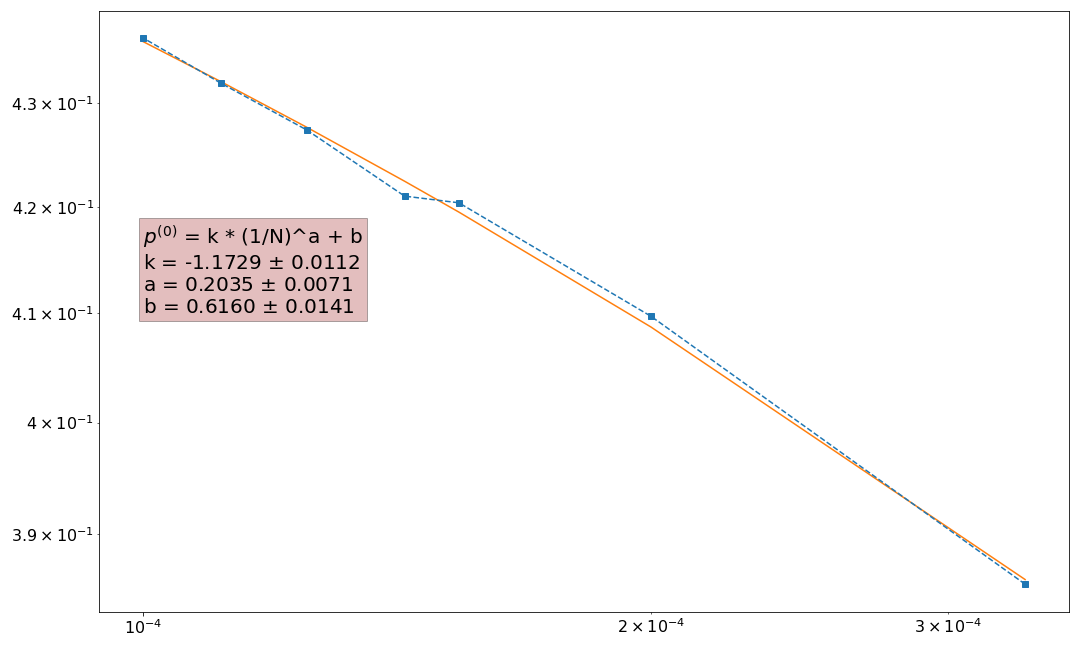
\includegraphics[width=\textwidth]{p0_res.png}
\caption{$p^{(0)}(N)$}
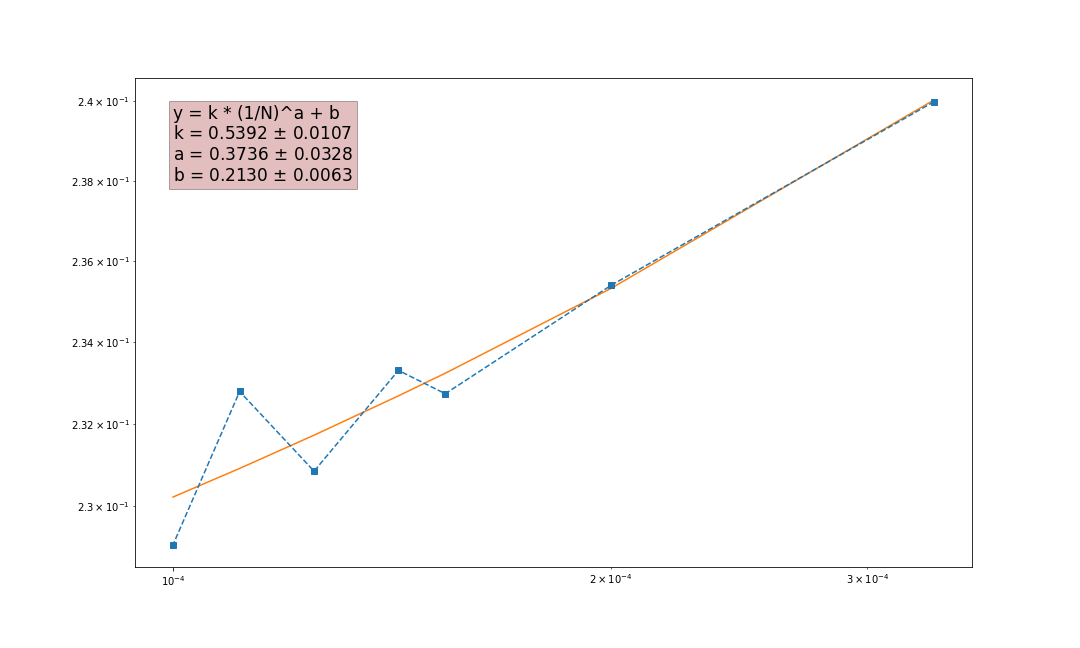
\includegraphics[width=\textwidth]{p1_res.png}
\caption{$p^{(1)}(N)$}
\end{subfigure}
\hfill
\begin{subfigure}{0.495\textwidth}
\centering
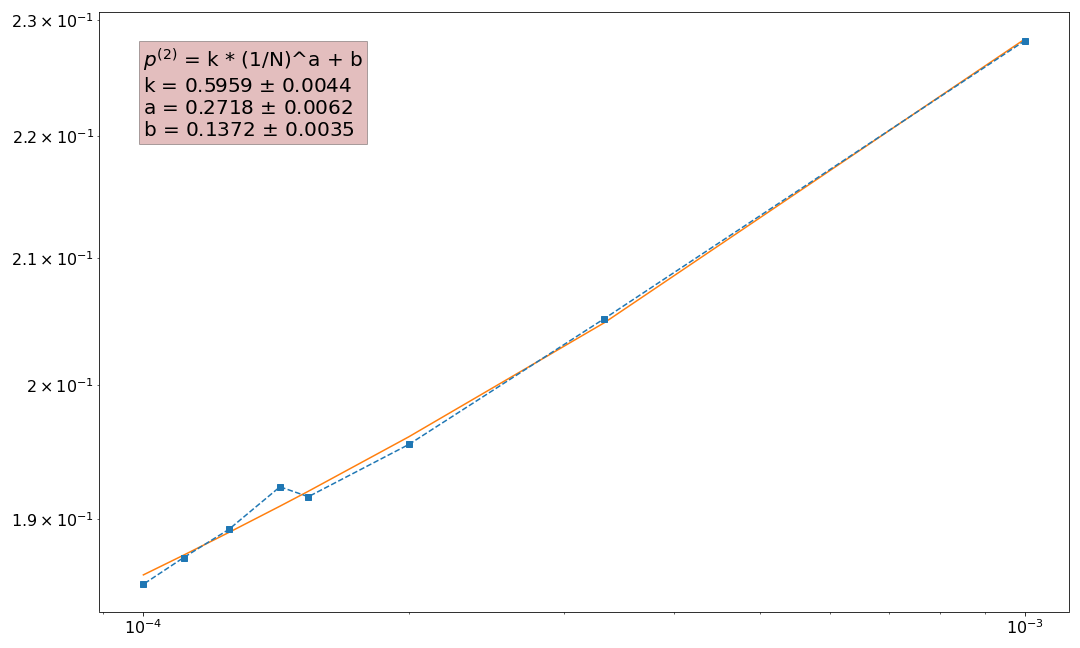
\includegraphics[width=\textwidth]{p2_res.png}
\caption{$p^{(2)}(N)$}
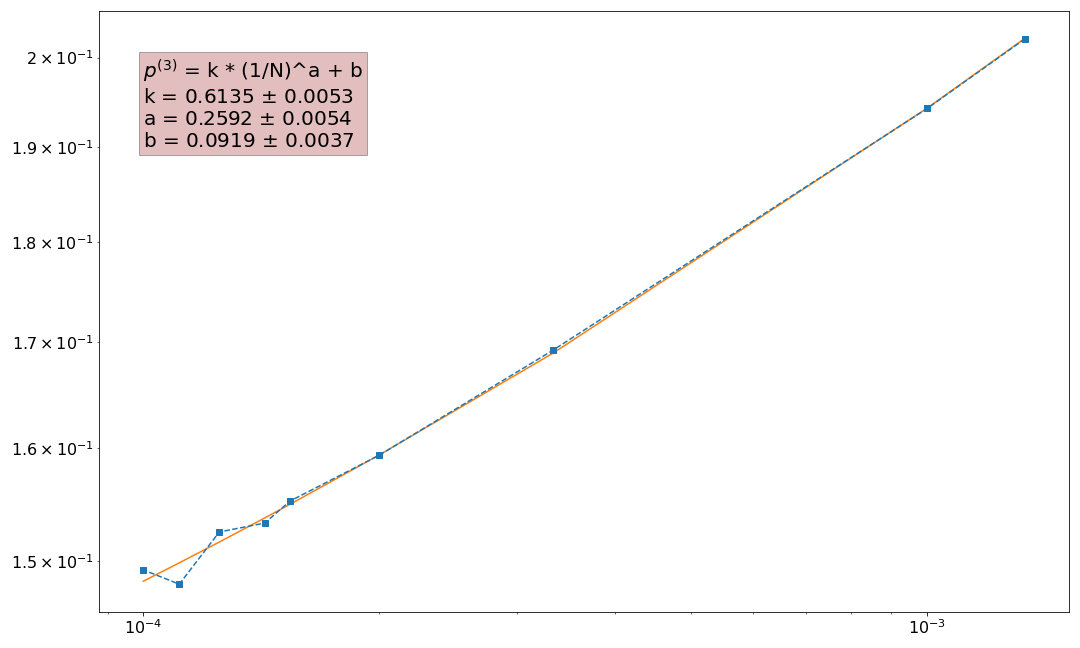
\includegraphics[width=\textwidth]{p3_res.png}
\caption{$p^{(3)}(N)$}
\end{subfigure}
\caption{Вероятности блуждания иметь атмосферу 0-3 от обратной длины конформации в степенном масштабе.}
\label{fig:p_03_loglog}
\end{figure}

Небольшие отклонения графиков апроксимирующей функции от прямолинейного вида обусловлены наличием ненулевого свободного линейного члена,
не входящего в классическую лог-лог регрессию $y = b * x^a$.
Больше всего сомнений вызывает график $p^{(1)}$ в виду сильных колебаний долей блужданий с атмосферой 1 при больших длинах.
Остальные графики $p^{(0)}$, $p^{(2)}$ и $p^{(3)}$ всё же подтверждают степенной (и что наиболее важно, с сильно отличными от нуля степенными коэффициентами) характер сходимости вблизи области бесконечно большой длины.

\subsection{Сравнение результатов вероятностей атмосфер от $N$ и $\Nun$}

Проведём, аналогично разделу \ref{sec:n_final}, численное сравнение коэффициентов шкалирующих функций $\pkn(N)$ и $\pkn(\Nun)$ из таблиц \ref{tab:p_i_log_log} и \ref{tab:p_i_u_log_log}.

\begin{table}[h]
\centering
\begin{tabular}{|c|c|c|c|}
\hline
 & b & d & $p^{(i)}(N=10000)$ \\ \hline
$p^{(0)}$ &  0.62(1) & 0.59(2) &  0.436369\\ \hline
$p^{(1)}$ & 0.213(6) & 0.214(6) & 0.229075\\ \hline
$p^{(2)}$ & 0.137(4) & 0.141(3) & 0.185300\\ \hline
$p^{(3)}$ & 0.092(4) & 0.097(3) & 0.149256\\ \hline
\end{tabular}
\caption{Пределы шкалирующих функций вероятностей блужданий с фиксированной атмосферой (от 0 до 3, сверху вниз) от $N$ \eqref{eq:pi_N} (левый столбец), от $\Nun$ \eqref{eq:pi_Nu} (центральный столбец) и ближайшие к пределу результаты Монте-Карло из таблицы \ref{tab:randw_p_atm} (правый столбец).}
\label{tab:bd_atm_compare}
\end{table}

Как видно по таблице \ref{tab:bd_atm_compare}, все пределы шкалирующих функций \eqref{eq:pi_N}, \eqref{eq:pi_Nu} при $1/N \to \infty, 1/\Nun \to \infty$ равны в пределах погрешности.
Так же, как в случае с пределами долей узлов $n_i$ (таблица \ref{tab:bd_compare}), наблюдается сильное различие между ближайшими к пределу результатами симуляций (нижняя строка таблицы \ref{tab:randw_p_atm}).
Это показывает сильное влияние степенного шкалирования результатов вблизи нуля аргументов функций: чем меньше степенной коэффициент ($a$ и $s$ для $\pkn(N)$ и $\pkn(\Nun)$ соотвественно), тем больше абсолютная разница между пределом и ближайшим экспериментом (сильнее ''загиб'' функции у $1/N \to 0$, как видно на графиках \ref{fig:randw_p_full}).

\begin{table}[h]
\centering
\begin{tabular}{|c|c|c|}
\hline
 & a & s \\ \hline
$p^{(0)}$ & 0.202(7) & 0.25(1) \\ \hline
$p^{(1)}$ & 0.37(3) & 0.44(4) \\ \hline
$p^{(2)}$ & 0.272(6) & 0.323(7) \\ \hline
$p^{(3)}$ & 0.259(6) & 0.310(6) \\ \hline
\end{tabular}
\caption{Степенные коэффициенты шкалирующих функций вероятностей блужданий с фиксированной атмосферой (от 0 до 3, сверху вниз) от $N$ \eqref{eq:pi_N} (левый столбец), от $\Nun$ \eqref{eq:pi_Nu} (правый столбец).}
\label{tab:as_atm_compare}
\end{table}

При сравнении коэффициентов $a$ и $s$ функций \eqref{eq:pi_N} и \eqref{eq:pi_Nu} соответственно, проиллюстрированном в таблице \ref{tab:as_atm_compare}, численное равенство между функциями одинаковых величин почти не наблюдается.
Исключением является пара $a_1$ и $s_1$, касающиеся друг друга в пределах погрешностей, но в отсутствии закономерностей среди других величин, совпадение может быть случайно.
С другой стороны, аналогично сравнению степенных коэффициентов функций долей узлов \eqref{eq:pi_N} и \eqref{eq:pi_Nu} в разделе \ref{sec:n_final}, наблюдается соразмерность степенных коэффициентов ($a_1 > a_2 > a_3 > a_0$ и $s_1 > s_2 > s_3 > s_0$). 
Заметно также, что все степенные коэффициенты $s$ функций $\pkn(\Nun)$ больше аналогичных коэффициентов $a$ функций от $N$.
Получим, что число уникальных узлов $\Nun$ с точки зрения степенного коэффициента является более сильным аргументом для функций вероятностей $\pkn$, что логично, ведь атмосфера блуждания напрямую зависит от заполненности решетки посещёнными или уникальными узлами.

\begin{table}[h]
\centering
\begin{tabular}{|c|c|c|}
\hline
 & k & q \\ \hline
$p^{(0)}$ & -1.17(1) &  -1.142(9) \\ \hline
$p^{(1)}$ & 0.54(1) & 0.52(1) \\ \hline
$p^{(2)}$ & 0.596(4) & 0.585(5) \\ \hline
$p^{(3)}$ & 0.613(5) & 0.604(5) \\ \hline
\end{tabular}
\caption{Линейные коэффициенты шкалирующих функций вероятностей блужданий с фиксированной атмосферой (от 0 до 3, сверху вниз) от $N$ \eqref{eq:pi_N} (левый столбец) и от $\Nun$ \eqref{eq:pi_Nu} (правый столбец).}
\label{tab:kq_atm_compare}
\end{table}

Линейные коэффициенты $k, q$  функций \eqref{eq:pi_N} и \eqref{eq:pi_Nu} изображены для наглядности на таблице \ref{tab:kq_atm_compare} и так же содержат схожие друг другу закономерности.
Коэффициенты при $p^{(1)}$ чуть касаются друг друга в пределах погрешности, при $p^{(2)}$ линейные показатели близки, но чуть-чуть расходятся в пределах ошибок, в то время как $k_3$ и $q_3$ равны в пределах погрешности.
Пара коэффициентов $k_0$ и $q_0$ сильно отличаются по сравнению с ошибками, однако имеют одинаковый отрицательный знак.

В итоге мы наблюдаем ожидаемое равество пределов $p^{(i)}$ как функций от $N$ \eqref{eq:pi_N}, так и от $\Nun$ \eqref{eq:pi_Nu}. 
Остальные поведенческие показатели (линейные и степенные) отличаются, что говорит об отсутствии полной численной взаимозаменяемости таких величин, как число шагов блуждания $N$ и число уникальных узлов блуждания $\Nun$.
Несмотря на это, функции величин от обоих аргументов универсальны по пределу и в знаковом поведении.
Это позволило увидеть большую информативность числа уникальных узлов $\Nun$ как аргумента наблюдаемых величин.

\section{Сравнение поведения атмосфер блужданий $\pkn$ и долей узлов $n_i$ модели RW}

Формула \eqref{eq:pkn}, описывающая атмосферу $a_t$ блуждания модели RW через число соседей конца блуждания $n_end$, ранее исследованное в разделе \ref{sec:neigh}, указывает на возможное сходство свойств модели RW.
Очевидно, атмосфера характеризует локальное координационное число блуждания в его конечном узле, однако сходство необходимо искать между долей узлов с $v$ соседями и вероятностью $4-v$ атмосферы блуждания, где $v=\{1,2,3,4\}$.
В данном разделе будет проведено сравнение ранее полученных результатов для долей узлов $n_i$ (в разделе \ref{sec:neigh}) и вероятностей атмосферы $\pkn$ (в разделе \ref{sec:atm}). 
Сравнение будет проведено для каждой группы функций по отдельности: для функций от $N$ (формула \eqref{eq:n_i_log_log} и \eqref{eq:pi_N}) и от $\Nun$ (формула \eqref{eq:n_i_u_log_log} и \eqref{eq:pi_Nu})

\subsection{Сравнение функций от $\Nun$}

Рассмотрим оценки коэффициентов шкалирующих функций от $\Nun$ (таблицы \ref{tab:n_i_u_log_log} для $n_i$ и \ref{tab:p_i_u_log_log} для $\pkn$).

\begin{table}[h]
\centering
\begin{tabular}{|c|c|c|c|}
\hline
v & $d(n_v)$ & $d(p^{(4-v)})$ \\ \hline
1 & 0.015(1) & 0.097(3) \\ \hline
2 & 0.053(2) & 0.141(3) \\ \hline
3 & 0.203(2) & 0.214(6) \\ \hline
4 & 0.741(5) & 0.59(2) \\ \hline
\end{tabular}
\caption{Пределы шкалирующих функций от $\Nun$: долей узлов с $v$ соседями (центральный столбец) и вероятностей блужданий с фиксированной атмосферой $4-v$ (правый столбец) от $\Nun$ (столбцы $d$ в таблицах \ref{tab:n_i_u_log_log} для $n_i$ и \ref{tab:p_i_u_log_log} для атмосфер).}
\label{tab:n_vs_atm_d}
\end{table}

По таблице \ref{tab:n_vs_atm_d} видно, что несмотря на соразмерность пределов, в границах погрешностей они значительно отличаются.  

\begin{table}[h]
\centering
\begin{tabular}{|c|c|c|c|}
\hline
v & $s(n_v)$ & $s(p^{(4-v)})$ \\ \hline
1 & 0.479(2) & 0.310(6) \\ \hline
2 & 0.214(1) & 0.323(7) \\ \hline
3 & 0.244(2) & 0.44(4) \\ \hline
4 & 0.225(4) & 0.25(1) \\ \hline
\end{tabular}
\caption{Степенные коэффициенты шкалирующих функций от $\Nun$: долей узлов с $v$ соседями (центральный столбец) и вероятностей блужданий с фиксированной атмосферой $4-v$ (правый столбец) от $\Nun$ (столбцы $s$ в таблицах \ref{tab:n_i_u_log_log} для $n_i$ и \ref{tab:p_i_u_log_log} для атмосфер).}
\label{tab:n_vs_atm_s}
\end{table}

Сравнение степенных коэффициентов (см. таблицу \ref{tab:n_vs_atm_s}) так же не показывает какого-либо численного сходства  между величинами - все значения значительно отличаются друг друга больше чем их погрешность.

\begin{table}[h]
\centering
\begin{tabular}{|c|c|c|c|}
\hline
v & $q(n_v)$ & $q(p^{(4-v)})$ \\ \hline
1 & 0.313(1) & 0.604(5) \\ \hline
2 & 0.567(3) & 0.585(5) \\ \hline
3 & 0.542(5) & 0.52(1) \\ \hline
4 & -1.20(1) & -1.142(9) \\ \hline
\end{tabular}
\caption{Линейные коэффициенты шкалирующих функций от $\Nun$: долей узлов с $v$ соседями (центральный столбец) и вероятностей блужданий с фиксированной атмосферой $4-v$ (правый столбец) от $\Nun$ (столбцы $s$ в таблицах \ref{tab:n_i_u_log_log} для $n_i$ и \ref{tab:p_i_u_log_log} для атмосфер).}
\label{tab:n_vs_atm_q}
\end{table}

Среди линейный коэффициентов (см. таблицу \ref{tab:n_vs_atm_q}) заметно лишь поведенческое сходство в виде одинаковых знаков рассматриваемых пар коэффицентов. В остальном так же численное сходство отсутствует.

\subsection{Сравнение функций от $N$}

Далее рассмотрим оценки коэффициентов шкалирующих функций от $N$ (данные взяты из таблиц \ref{tab:n_i_log_log} для $n_i$ и \ref{tab:p_i_log_log} для $\pkn$). Аналогично прошлому разделу, сравниваться будут пары среди свободных коэффициентов или пределы функций (таблица \ref{tab:n_vs_atm_b}), степенные коэффициенты (таблица \ref{tab:n_vs_atm_a}) и, наконец, линейные коэффициенты (таблица \ref{tab:n_vs_atm_k})

\begin{table}[h]
\centering
\begin{tabular}{|c|c|c|c|}
\hline
v & $b(n_v)$ & $b(p^{(4-v)})$ \\ \hline
1 & 0.014(1) & 0.092(4) \\ \hline
2 & 0.037(2) & 0.137(4) \\ \hline
3 & 0.202(3) & 0.213(6) \\ \hline
4 & 0.759(5) & 0.62(1) \\ \hline
\end{tabular}
\caption{Пределы шкалирующих функций от $N$: долей узлов с $v$ соседями (центральный столбец) и вероятностей блужданий с фиксированной атмосферой $4-v$ (правый столбец) от $\Nun$ (столбцы $b$ в таблицах \ref{tab:n_i_log_log} для $n_i$ и \ref{tab:p_i_log_log} для атмосфер).}
\label{tab:n_vs_atm_b}
\end{table}

\begin{table}[h]
\centering
\begin{tabular}{|c|c|c|c|}
\hline
v & $a(n_v)$ & $a(p^{(4-v)})$ \\ \hline
1 & 0.417(2) & 0.259(6) \\ \hline
2 & 0.171(1) & 0.272(6) \\ \hline
3 & 0.219(3) & 0.37(3) \\ \hline
4 & 0.189(3) & 0.202(7) \\ \hline
\end{tabular}
\caption{Степенные коэффициенты шкалирующих функций от $N$: долей узлов с $v$ соседями (центральный столбец) и вероятностей блужданий с фиксированной атмосферой $4-v$ (правый столбец) от $\Nun$ (столбцы $s$ в таблицах \ref{tab:n_i_log_log} для $n_i$ и \ref{tab:p_i_log_log} для атмосфер).}
\label{tab:n_vs_atm_a}
\end{table}

\begin{table}[h]
\centering
\begin{tabular}{|c|c|c|c|}
\hline
v & $k(n_v)$ & $k(p^{(4-v)})$ \\ \hline
1 & 0.3425(8) & 0.613(5) \\ \hline
2 & 0.573(4) & 0.596(4) \\ \hline
3 & 0.588(3) & 0.54(1) \\ \hline
4 & -1.239(9) & -1.17(1) \\ \hline
\end{tabular}
\caption{Линейные коэффициенты шкалирующих функций от $N$: долей узлов с $v$ соседями (центральный столбец) и вероятностей блужданий с фиксированной атмосферой $4-v$ (правый столбец) от $N$ (столбцы $k$ в таблицах \ref{tab:n_i_log_log} для $n_i$ и \ref{tab:p_i_log_log} для атмосфер).}
\label{tab:n_vs_atm_k}
\end{table}

Сравнение функций от $N$ так же показало отсутствие численного сходства коэффициентов или какой-либо закономерности среди групп значений. 
Исключением оказалось аналогичное группе функций от $\Nun$ сходство знаков линейных коэффициентов.
По остальным возможным признакам сходства корреляция не наблюдается.

\subsection{Итоги сравнения}

О связи между долей узлов с фиксированным числом соседей $\la n_v \ra$ и вероятностью атмосферы $p^{(4-v)_N}$ ублуждания RW существует говорит совсем немного аргументов.
Во-первых, это подтверждённый степенной характер аппроксимации обеих величин как относительно числа шагов блуждания $N$, так и относительно числа уникальных узлов $\Nun$.
Во-вторых, это схожесть знаков линейных коэффициентов. 
Однако, если она и существует, против чего говорит полное отсутствие численного сходства между коэффициентами, то крайне слабая, ввиду разной статистической мощности наблюдаемых величин. 
Очевидно, что $\la n_v \ra$ охватывает геометрическое поведение всего блуждания, в то же как $\la p^{(v)} \ra$ описывает поведение лишь на его концах, характер которых с увеличением длины блуждания становится некоррелируемым с поведением внутренних узлов.

Не подтвердилась так же и универсальность свойств локального координационного числа по отношению с SAW-модели, где пределы долей узлов и вероятностей атмосфер бесконечно-больших блужданий имели значительно большее сходство (раздел \ref{sec:Prellberg}), нежели в данной модели.

\subsection{Планируемая деятельность}

\begin{itemize}
\item 3-я итерация программного кода для симуляции модели Rand-Walk - добавление в модель аналога квадратной решётки с целью упрощения расчётов уникальных узлов и их соседей.
\end{itemize}

\section{Критическое поведение модели IsingISAW на треугольной решётке}

В данном разделе проводится исследование критической области модели Изинга на случайном блуждания без самопересечений на треугольной решётке (далее, TrIsingISAW).
В отличие от классической модели на квадратной решётке, узлы треугольной решётки имеют две дополнительные связи по одной из диагоналей (см. рисунок \ref{fig:lattices}), 
вследствие чего координационное число данной модификации (кол-во возможных связей у одного узла) увеличено по сравнению с квадратной с 4 до 6.

\subsection{Поиск точки фазового перехода}

\begin{equation}
\label{eq:IsISAW_H}
 H_{N,u,\{\sigma\}} = -\sum_{i,j} J\sigma_i \sigma_j, i,j \in u, |u| = N
\end{equation}

\begin{equation}
\label{eq:TrIsISAW_E}
\la \epsilon \ra = \la H \ra / N
\end{equation}

Были проведены симуляции Монте-Карло при нулевом внешнем поле и $J \in [0,0.9]$. 
Итоговое количество шагов симуляций от $10^10$ до $10^11$, симулированные блуждания имеют длину $N$ от 100 до 7200.
Были собраны данные для удельной энергии системы на спин $\la \epsilon \ra$ \eqref{eq:TrIsISAW_E} и средняя 2-я и 4-я степени намагниченности на спин $\la m^2 \ra$, $\la m^4 \ra$.
Так же собрана статистика среднего расстояния между концами блуждания $R^2_N$.

\begin{equation}
\label{eq:IsISAW_m2}
	m^{k} = (\sum_{i \in u} \sigma_i / N)^k
\end{equation}

\begin{figure}[h]
\begin{subfigure}{0.49\textwidth}
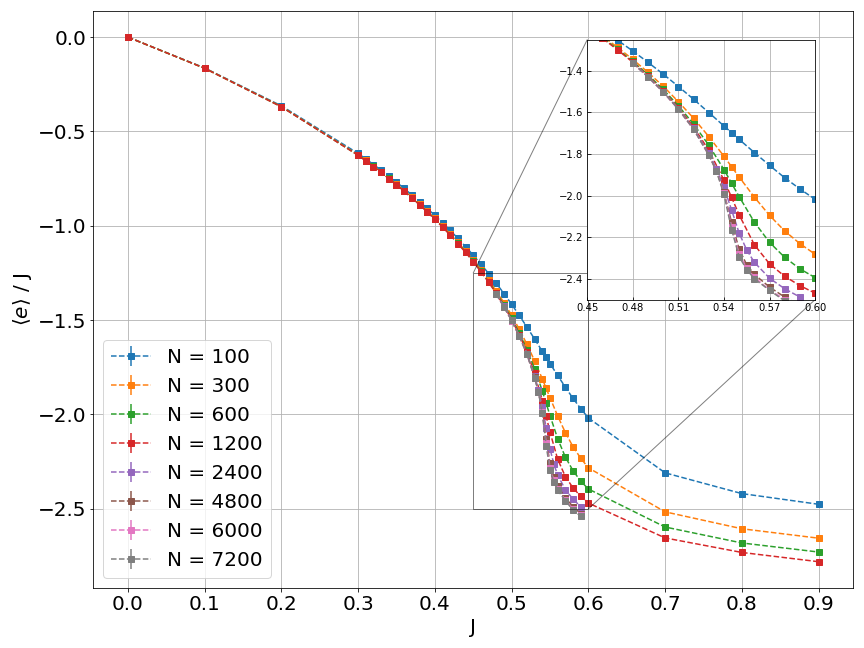
\includegraphics[width=\textwidth]{TrIsISAW_E.png}
\caption{}
\label{fig:TrIsISAW_E}
\end{subfigure}
\hfill
\begin{subfigure}{0.49\textwidth}
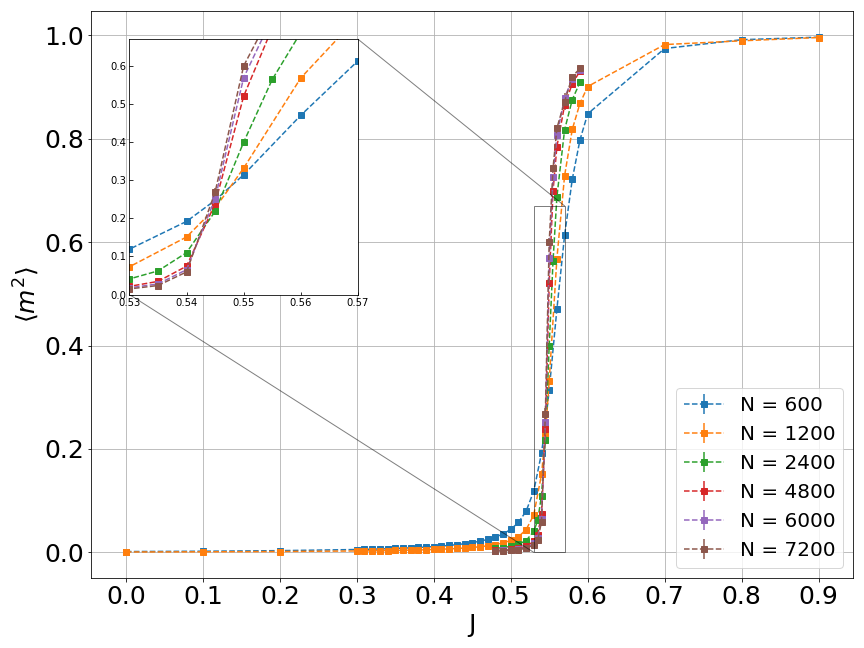
\includegraphics[width=\textwidth]{TrIsISAW_m2.png}
\caption{}
\label{fig:TrIsISAW_m2}
\end{subfigure}
\caption{Слева: удельная энергия узла \eqref{eq:TrIsISAW_E} модели TrIsingISAW (без учёта константы $J$).
Справа: средняя вторая степень намагниченности \eqref{eq:IsISAW_m2} узла модели TrIsingISAW. 
Длины конформаций в обоих графиках от 100 до 7200 (длины отмечены разными цветами)}

\end{figure}

На графике \ref{fig:TrIsISAW_E} показана зависимость удельной энергии \eqref{eq:TrIsISAW_E} узла модели TrIsingISAW.
График показывает что удельная энергия системы стремится к -3J в пределе бесконечной длины конформации, 
что логично, поскольку с ростом $J$ узлы приобретают наиболее возможное число связей (то есть, 6), но так как св
язи существуют между парами узлов,
необходимо поделить число связей на 2.
При малых $J$ энергия почти не зависит от длины цепочки $N$, но начиная с $J > 0.53$, расхождение графиков становится наиболее четким.

На графике \ref{fig:TrIsISAW_m2} изображен момент намагниченности второго порядка \eqref{eq:IsISAW_m2} в зависимости от $J$.
Графики величины для конформаций разных длин имеют четкое пересечение в $J \approx 0.545$.

\begin{equation}
\label{eq:IsISAW_U4}
	U_4 = 1 - \frac{\la m^4 \ra}{3 \la m^2 \ra}
\end{equation}

\begin{figure}[h]
\begin{subfigure}{0.49\textwidth}
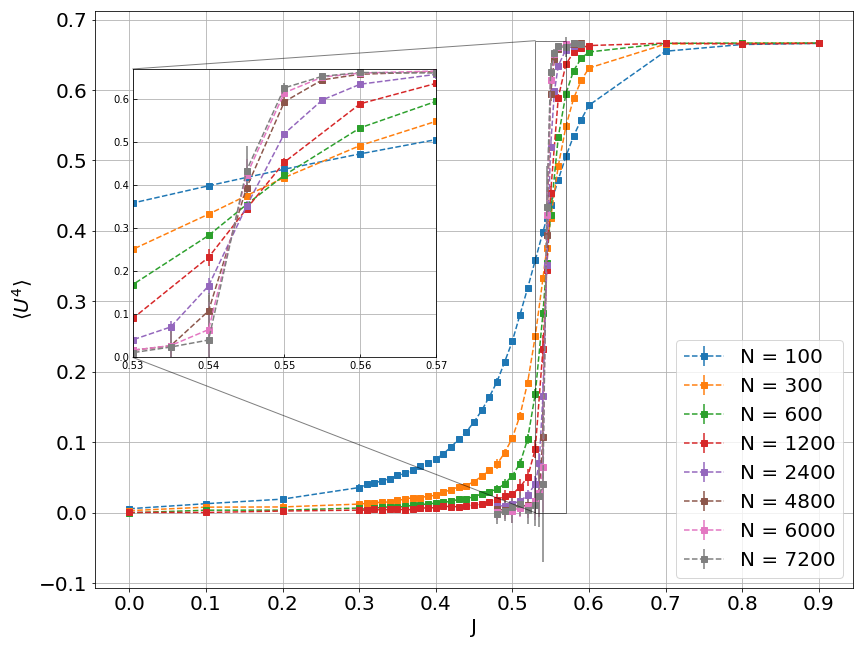
\includegraphics[width=\textwidth]{TrIsISAW_U4.png}
\caption{}
\label{fig:TrIsISAW_U4}
\end{subfigure}
\hfill
\begin{subfigure}{0.49\textwidth}
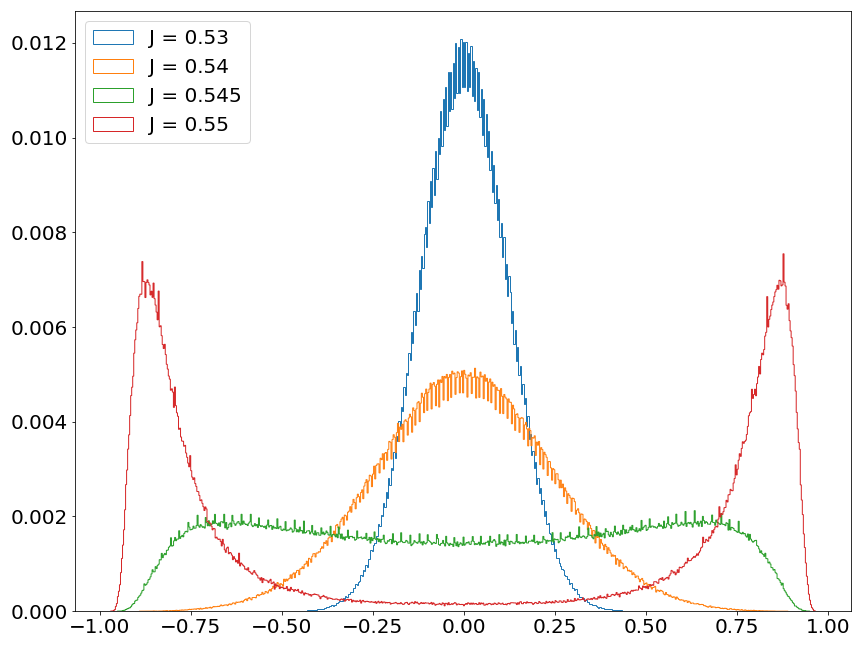
\includegraphics[width=\textwidth]{TrIsISAW_m2_distr.png}
\caption{}
\label{fig:TrIsISAW_m2_distr}
\end{subfigure}
\caption{Слева: кумулянт Биндера модели TrIsingISAW с длиной конформации от 100 до 7200 (длины отмечены разными цветами).
Справа: распределение удельной намагниченности модели TrIsingISAW на конформации длиной $N=7200$ при $J \in [0.53,0.55]$ (значения J отмечены разными цветами)}
\end{figure}


График \ref{fig:TrIsISAW_U4} показывает зависость кумулянта Биндера \eqref{eq:IsISAW_U4} от J. 
Пересечение графиков от конформаций разных длин, соответствующее переходу от парамагнетических к ферромагнетическим свойствам, снова наблюдается в $J \approx 0.545$.

Распределение значений удельной намагниченности для модели TrIsingISAW изображено на графике \ref{fig:TrIsISAW_m2_distr}.
График показывает, что распределение с преобладающими малыми по модулю значениями удельной намагниченности уступают 
распределениям с преобладающими крайними значениями намагниченности возле $J=0.545$, где распределение близко к почти равномерному.


\begin{figure}[h]
\begin{subfigure}{0.49\textwidth}
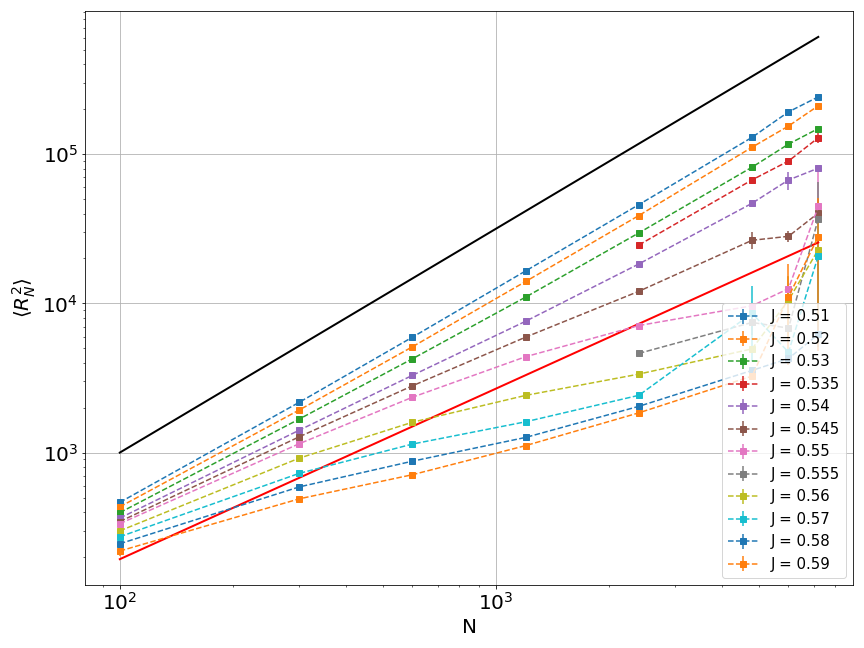
\includegraphics[width=\textwidth]{TrIsISAW_R2log.png}
\caption{}
\label{fig:TrIsISAW_R2log}
\end{subfigure}
\hfill
\begin{subfigure}{0.49\textwidth}
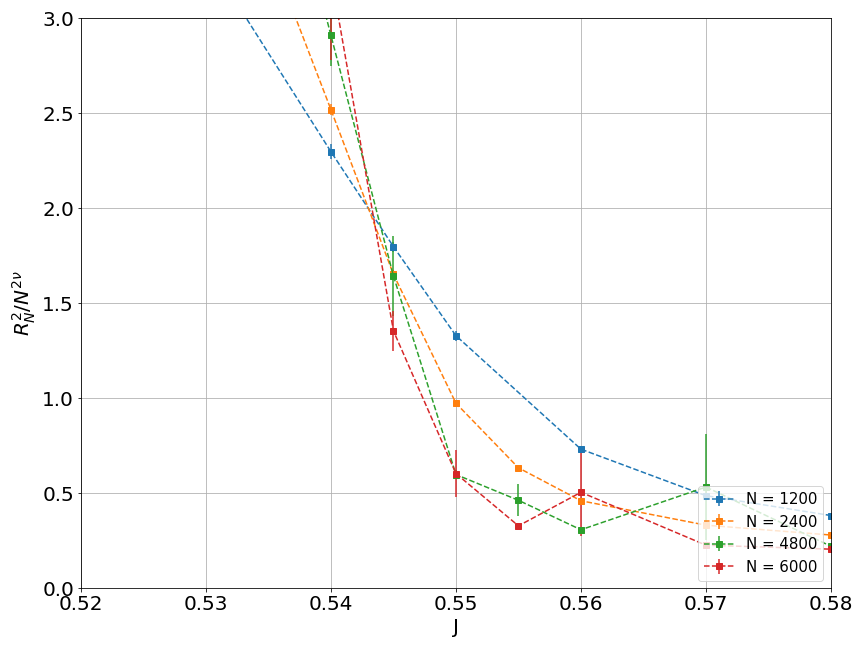
\includegraphics[width=\textwidth]{TrIsISAW_R2toN2v.png}
\caption{}
\label{fig:TrIsISAW_R2toN2v}
\end{subfigure}
\caption{Слева: Расстояние между концами блужданий длины $N$ при $J \in [0.51,0.59]$ в логарифмическом масштабе. 
Для наглядности добавлены линии $N^{2\nu}$, где $\nu = 4/7$ (красная линия) и $\nu=3/4$ (чёрная линия).
Справа: отношение расстояния между концами блуждания $R^2$ к $N^{2\nu}$, где $\nu=3/4$ при $J \in [0.52,0.58]$}
\end{figure}

Рассмотрим так же конформационный переход модели.
Рисунок \ref{fig:TrIsISAW_R2log} описывает расстояние между концами блужданий модели TrIsingISAW как функцию длины блуждания при фиксированном значении J.
Функции изображены в логарифмическом масштабе для наглядного наблюдения степенного шкалирования величины при $N \to \infty$.
Так же для сравнения были добавлены прямые $N^{2\nu}$, где $\nu = 4/7$ (красная линия) - константа поведения модели ISAW на квадратной решетке в точке критического перехода \cite{Duplantier1987},
и $\nu = 3/4$ (черная линия) - константа поведения невзаимодействующего блуждания без самопересечений \cite{Rensburg2015}.
На рисунке видно, что при $J \leq 0.53$ поведение графиков близко к чёрной линии, в то время как графики с $J = 0.54, 0.545$ в значительной степени схожи к красной линией.
У графиков с большим значением $J$, наблюдается сильное снижение наклона прямой, что говорит о более сжатом состоянии блужданий при $J \geq 0.55$.  

График \ref{fig:TrIsISAW_R2toN2v} описывает ту же величину, но перешкалированную относительно $N^{2\nu}$ в зависимости от $J$.
Результаты показывают, что вблизи точки $J = 0.543$ величина $R^2 / N^{2\nu}$ становится N-независимой. 

Таким образом, на основании пронаблюдаемых магнитного (рисунки \ref{fig:TrIsISAW_U4} и \ref{fig:TrIsISAW_m2_distr}) и конформационного (рисунок \ref{fig:TrIsISAW_R2log}) переходов,
точка фазового перехода модели предполагается возле точки $J=0.545$. Считая погрешностью оценки расстояние между измерениями, итоговая оценка точки фазового перехода:

\begin{equation}
\label{eq:TrIsISAW_Jc}
	J_c = 0.545(5)
\end{equation}

Для оценки критического кумулянта, ввиду слишком большой наблюдаемой погрешности, требуются более длительные симуляции длин $N > 5000$.


\newpage

\subsection{Критические экспоненты модели}

В данном подразделе критическое поведение модели TrIsingISAW будет исследовано в сравнении с оригинальной модификацией модели IsingISAW на квадратной решётке, рассмотренной ранее в статье \cite{faizullina2021critical}.
Прошкалируем наблюдаемые величины $\la R^2 \ra$ и $m^2$ относительно соотвествующих критических экспонент:
так, величины вблизи предполагаемой точки фазового перехода рассматриваются как функции:

\begin{equation}
\begin{array}{l}
\label{eq:TrIsISAW_datcoll}
\la R^2 \ra = N^{2\nu} f(x), \\
\la m^2 \ra = N^{-2\beta\phi} g(x), \\
x = (J-J_c) N^{\phi},
\end{array}
\end{equation}

где $\nu$, $\phi$, $\beta$  - пространственный, переходный, и порядковый показатели соответственно, в то время как $f(x)$ и $g(x)$ - безразменные шкалирующие функции безразмерной величины.
В рамках последующего анализа коллапса данных, подберём наилучшие критические показатели и точку фазового перехода, 
чтобы получить наиболее визуально гладкие функции $f(x)$ и $g(x)$ вблизи $x=0$.


\begin{figure}[h]
\begin{subfigure}{0.49\textwidth}
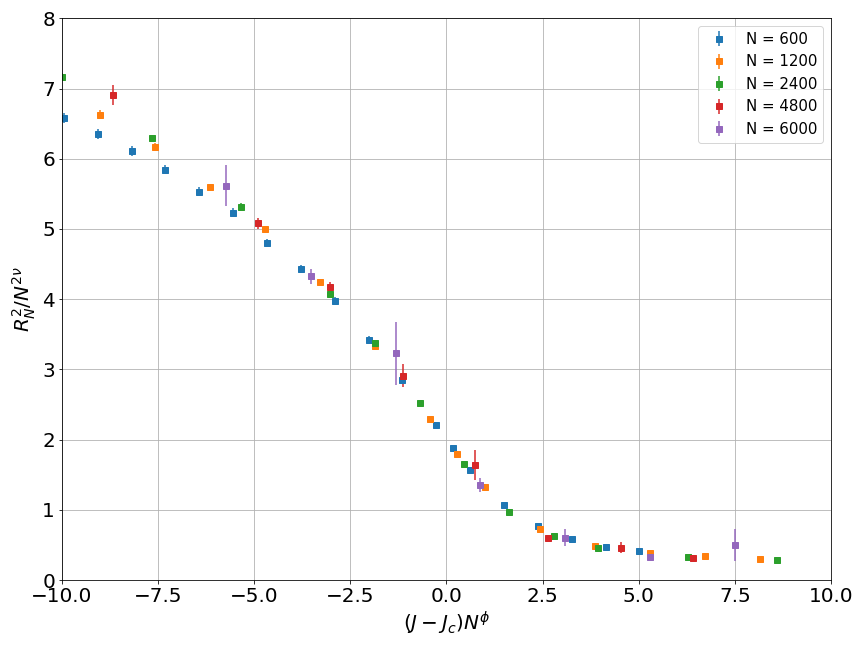
\includegraphics[width=\textwidth]{TrIsISAW_R2_datcoll.png}
\caption{}
\label{fig:TrIsISAW_R2_datcoll}
\end{subfigure}
\hfill
\begin{subfigure}{0.49\textwidth}
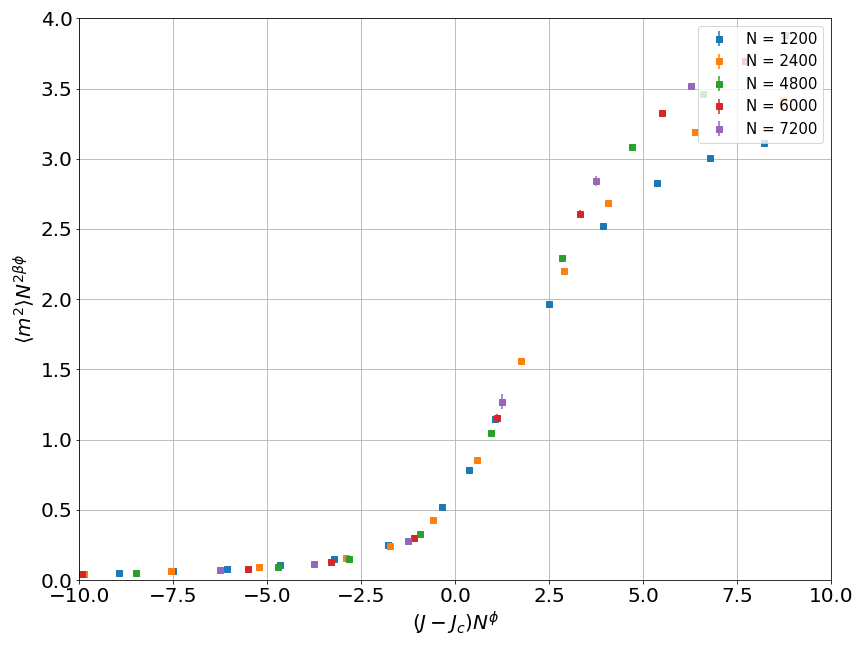
\includegraphics[width=\textwidth]{TrIsISAW_m2_datcoll.png}
\caption{}
\label{fig:TrIsISAW_m2_datcoll}
\end{subfigure}
\caption{Коллапс данных наблюдаемых величин модели TrIsingISAW.
Слева: Расстояние между концами блужданий $\la R^2_N \ra$, при $\nu = 4/7$, $\phi=0.7$, $J_c = 0.543$, N=[600, 6000].
Справа: Средняя вторая степень удельной магниченности $\la m^2 \ra$, при $\beta = 1/8$, $\phi=0.7$, $J_c = 0.5425$, N=[1200, 7200]}
\end{figure}

Графики \ref{fig:TrIsISAW_R2_datcoll} и \ref{fig:TrIsISAW_m2_datcoll} описывают наиболее гладко изображенные функции $f(x), g(x)$ \eqref{eq:TrIsISAW_datcoll}.
В качестве показателей были взяты результаты из работы \cite{faizullina2021critical}.
Результаты показывают, что использованные показатели при дополнительной коррекции точки фазового перехода $J_c$ дают достаточно чёткий коллапс данных.
Это подтвеждает универсальность критических экспонент родительских моделей Ising 2D (модель Изинга на двумерной решётке) 
и ISAW 2D (взаимодействующее бесспиновое случайное блуждание без самопересечений), из которых и были ранее взяты значения экспонент,
а также согласуется с оценкой критической точки выше \eqref{eq:TrIsISAW_Jc}.


\subsection{Вопросы}

\begin{itemize}
\item Статья 2021: что означает correction-to-scalling для графика $R^2 / N^{2\nu}$
\end{itemize}


\section{Критическое поведение взаимодействующего блуждания без самопересечений на треугольной решётке}

Основная цель данного раздела - исследование критических свойств модели ISAW на треугольной решётке (далее, TrISAW).
Данная задача решалась ранее, в статье \cite{Privman1986}, использованием приближений наблюдаемых величин рядями Тейлора.
Полученная оценка точки фазового перехода для TrISAW выписана на таблице \ref{tab:crits}.

В данном разделе мы воспользуемся известными данными о шкалировании радиуса между краями блуждания $R^2_N$:
на основании результатов о невзаимодействующем блуждании без самопересечений \cite{Rensburg2015}, а так же о критическом поведении взаимодействующего блуждания \cite{Duplantier1987} на квадратной решётке,
найдём область конформационного перехода модели и, тем самым, уточним оценку точки фазового перехода.
 

\begin{figure}[h]
\begin{subfigure}{0.49\textwidth}
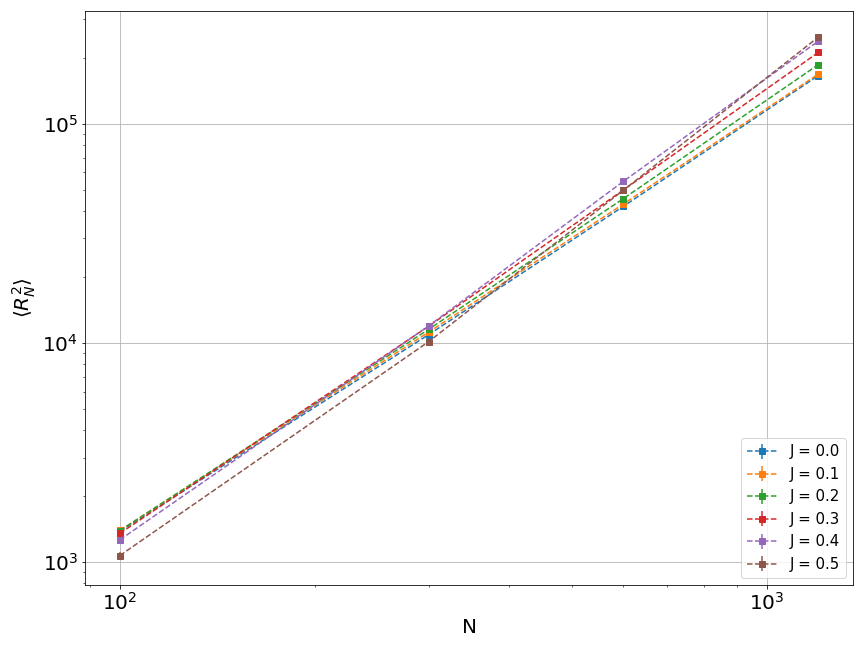
\includegraphics[width=\textwidth]{TrISAW_R2log.png}
\caption{}
\label{fig:TrISAW_R2log}
\end{subfigure}
\hfill
\begin{subfigure}{0.49\textwidth}
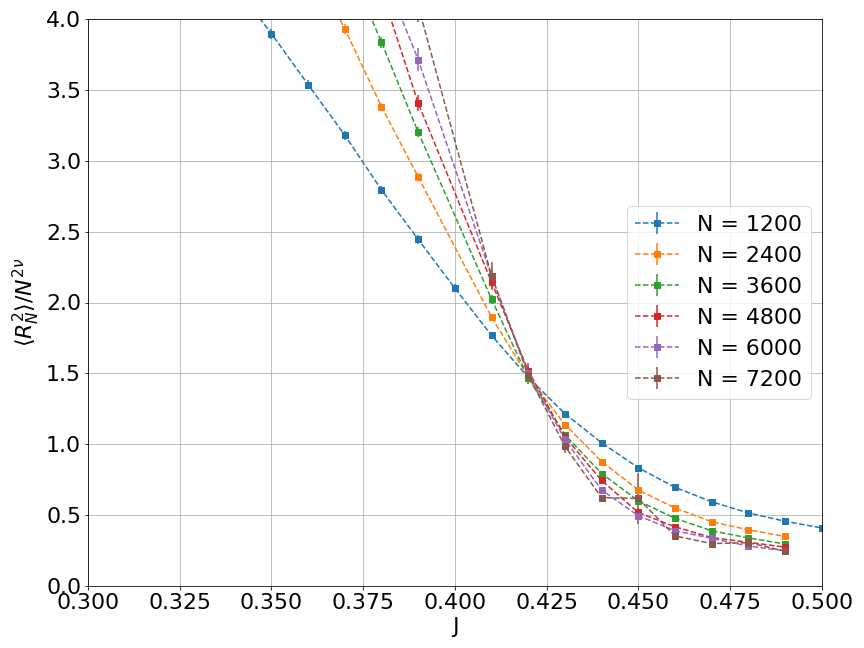
\includegraphics[width=\textwidth]{TrISAW_R2toN2v.png}
\caption{}
\label{fig:TrISAW_R2toN2v}
\end{subfigure}
\caption{Слева: Расстояние между концами блужданий длины $N$ при $J \in [0.51,0.59]$ в логарифмическом масштабе. 
Для наглядности добавлены линии $N^{2\nu}$, где $\nu = 4/7$ (красная линия) и $\nu=3/4$ (чёрная линия).
Справа: отношение расстояния между концами блуждания $R^2$ к $N^{2\nu}$, где $\nu=4/7$ при $J \in [0.52,0.58]$}
\end{figure}

\section{Заключение}

В ходе первой части работы было исследовано поведение локального координационного числа модели Изинга на СБС, а так же в модели взаимодействующего блуждания.
Плотность связей была рассмотрена в модели на нескольких решётках в зависимости от константы J,
а так же в состоянии нулевого взаимодействия в зависимости от длины цепочки.
Методами Монте-Карло был определён линейный характер зависимости средних долей локального координационного числа в блуждании (далее, долей ЛКЧ) от длины конформации и пределы долей на бесконечно большой длине цепочки.
Так же было проведено сравнение этих значений на предмет универсальности среди квадратной, треугольной, кубической и 4D-гиперкубической решёток: 
асимптотические пределы долей оказались численно различны среди разных решёток, однако по знаковому поведению Ising-ISAW на треугольной решётке имеет больше общего с кубической решёткой, имеющей одинаковое с треугольной координационное число, чем с квадратной, имеющей равную треугольной размерность. 

Для сравнения поведения ЛКЧ между внутренним и граничным узлом конформации в пределе бесконечно большой длины цепочки,
было проведено сравнение полученных для невзаимодействующей модели Ising-ISAW пределов средних долей ЛКЧ с предельными значениями вероятностей атмосфер невзаимодействующего блуждания на квадратной решётке из работы \cite{owczarek2008scaling}. 
Результат показал небольшую, но значимую впределах погрешностей разницу между величинами в пределе бесконечно длиной цепочки, 
что говорит о значительной различии поведений ЛКЦ в узлах близких в концами блужданий по сравнению с внутренними узлами цепочки. 

Чтобы рассмотреть влияние исключенного объёма на поведение локального координационного числа, аналогичное исследование было проведено для простого случайного блуждания на квадратной решётке.
Результаты симуляций показали степенной характер шкалирования долей ЛКЧ как от числа шагов случайного блуждания, 
так и от числа уникальных узлов блуждания.
Похожим свойством обладало и атмосфера простого случайного блуждания, 
несмотря на гораздо большее численное отличие шкалирующих показателей между величинами, чем в невзамодействующем СБС.

Так же проводилось исследование критических свойств моделей взаимодействующих полимеров на треугольных решётках.
Точка фазового перехода модели TrIsing-ISAW значительно отличается от $\theta$-точки оригинальной модели на квадратной решётке. 
С другой, стороны методом коллапса данных была подтверждена применимость ранее найденных критических показателей $\nu$ и $\phi$ для квадратных решёток в треугольных модификациях моделей, что говорит об универсальности ряди критических свойств среди двумерных решёток.
\section{Программно-техническое приложение}

В данном разделе будут описаны особенности работы с суперкомпьютером НИУ ВШЭ, которые могут быть важными дополнением к основной инструкции пользователя.

\subsection{Применение jit-компиляции при программировании на языке Python}
\label{subsection:njit_problem}

Симуляции случайного блуждания с самопересечениями (для кода см. папку $Random\_Walk$  \cite{web:ProjectMagnetRepos}) были запрограммированны на языке Python с компиляцией с помощью пакета numba метод jit. В качестве окружения была использована стандартная библиотека $Python/Anaconda\_v11.2021$ встроенная в стандартное ПО суперкомпьютера. 

Выполнение первых экспериментов по симуляциям шло крайне медленно - результаты за семь дней можно увидеть на таблице \ref{tab:Ran_Walk_neigh_1}

\begin{table}[h]
    \centering
    \begin{tabular}{|c|c|c|c|c|c|c|}
        \hline
        N & $steps$ & $unique$ & $n_{1}$ & $n_{2}$ & $n_{3}$ & $n_{4}$ \\ \hline
        100 & 7450000 & 0.49(8) & 0.07(3) & 0.33(9) & 0.36(7) & 0.24(9) \\ \hline
        200 & 5684000 & 0.44(7) & 0.05(2) & 0.29(7) & 0.35(5) & 0.30(9) \\ \hline
        500 & 2045000 & 0.39(6) & 0.04(1) & 0.24(5) & 0.34(4) & 0.38(8) \\ \hline
        1000 & 654000 & 0.36(5) & 0.03(1) & 0.22(4) & 0.33(4) & 0.42(7) \\ \hline
        2500 & 132000 & 0.33(4) & 0.027(7) & 0.19(3) & 0.31(3) & 0.48(6)  \\ \hline
        5000 & 37000 & 0.31(4) & 0.024(5) & 0.17(3) & 0.29(3) & 0.51(6) \\ \hline
        10000 & 10000 & 0.29(3) & 0.021(4) & 0.16(2) & 0.28(3) & 0.54(5) \\ \hline
    \end{tabular}
    \caption{Средние доли узлов c 1-4-мя соседями в конформациях модели Random-Walk длин $10^{2}-10^{4}$}
    \label{tab:Ran_Walk_neigh_1}
\end{table}

Для сравнения с другими платформами, в случае длины цепочки $N=10000$, процесс из 10000 шагов на Google Colab занимал не более 7 часов.

\begin{figure}[h]
    \centering
    
\includegraphics[width=0.95\textwidth]{experiment_time.png}
\end{figure}

Решением проблемы оказалось создание собственного окружения с другими версиями используемых пакетов numpy и numba (полный список так же есть в репозитории с кодом \cite{web:ProjectMagnetRepos}). Новые результаты за 7 дней описаны в продолжении основного раздела.

При обсуждении столь значительного различия во времени выполнениями между окружениями поддержкой было выдвинуто предположение, что окружения отличаются сторонними библиотеками линейной алгебры, используемой пакетом numpy: наиболее распространенными считаются OpenBLAS и Intel MKL. Основным фактором преимущества той или иной библиотеки является именно процессор (Intel или non-Intel). 

В новом окружении пакетом numpy использовалась именно библиотека OpenBLAS, в то время как в Anaconda - Intel MKL. Это следовало из применения в данных окружениях следующего:

\begin{code}
import numpy

print(numpy.show\_config())
\end{code}

Подробнее об определении какая библиотека линейной алгебры используется в пакете numpy можно найти \href{https://shaalltime.medium.com/benchmark-numpy-with-openblas-and-mkl-library-on-amd-ryzen-3950x-cpu-96184f91057f}{здесь}. 


\subsection{Итерации программного комплекса Rand-Walk}

Подраздел посвящён описанию версий программного комплекса для симуляций модели простого случайного блуждания фиксированной длины N на квадратной решётке.
(для кода см. папку $Random\_Walk$  \cite{web:ProjectMagnetRepos})

\begin{enumerate}
\item \textbf{Drunken\_Sailor\_def.py} - базовый алгоритм симуляций, предназначенный для проверки работы основных функций: 
\begin{itemize}
\item experiment - генерация цепочки и подсчёт наблюдаемых (доли узлов с числом соседей 1-4, а так же доля уникальных узлов цепочки)
\item \textit{complex\_experiment} - запись результирующего массива для одной цепочки (experiment) и набора цепочек (шаг - кол-во опытов между анализом данных)
\item \textit{write\_results} - запись текущих результатов (средних наблюдаемых по всем экспериментам) в текстовый файл
\item \textit{save\_distr} - распределение значений наблюдаемых по всем экспериментам
\item \textit{save\_history} - сохранение истории средний значений для анализа сходимости результаотв симуляций
\end{itemize}
Цепочка генерируется как двумерный массив точек, потому наиболее его медленной частью является поиск уникальных узлов цепочки через \textit{np.unique}, не поддерживающий njit-комплиляцию при обработке двумерного массива.
\item \textbf{Drunken\_Sailor.py} - первая версия симуляционного комплекса с jit-компилируемой частью. Алгоритмически не отличается от \textbf{Drunken\_Sailor\_def.py}, но значительно быстрее базовой версии
\item \textbf{Drunken\_Sailor\_v2.py} - оптимизированная версия \textbf{Drunken\_Sailor.py} c расширенной njit-комплиляцией:
\begin{itemize} 
\item \textit{create\_walk} - генерация цепочки как массива поворотов блуждания начиная с начальной точки $(0,0)$, затем - как массив всех точек блуждания
\item \textit{calc\_fractions} - основная функция подсчёта наблюдаемых. Так же модифицирована над подсчёт атмосферы каждого блуждания
\item В \textit{complex\_experiment} добавлено распараллеливание проведение набора экспериментов за шаг между выводом данных, что позволило значительно ускорить работу комплекса.
\item \textit{stats} - подсчёт текущего результата для наблюдаемых долей
\item \textit{atm\_bins} - подсчёт долей блужданий с атмосферой 0-3
\end{itemize}
\end{enumerate}


\bibliographystyle{plain}
\bibliography{bibliography}

%\fi

\end{document}



